% Copyright 2026 Sreeram Anil
% SPDX-License-Identifier: CC-BY-4.0
% =============================================================================
%  ROBUST / EMBEDDED KALMAN family — chapter index
%
%  Order: (1) parameter uncertainty, (2) worst-case design, (3) the three
%  residual-reweighting M-estimators (Huber -> correntropy -> Student's t, in
%  order of increasing rejection depth), (4) hard state constraints,
%  (5) model-order reduction, (6) the sliding-mode (non-stochastic) filter.
%
%  Bibliography keys come from report/refs.bib and
%  report/refs_additions_robust_kalman.bib.
% =============================================================================

% Notation macros used by this family that are not in report/preamble.tex.
% \providecommand is idempotent, so the chapter files may (and do) repeat them.
\providecommand{\vf}{\bm{f}}   % model transition function
\providecommand{\vh}{\bm{h}}   % model output function
\providecommand{\vd}{\bm{d}}   % stacked regression data vector
\providecommand{\mM}{\bm{M}}   % stacked regression matrix
\providecommand{\va}{\bm{a}}
\providecommand{\vb}{\bm{b}}

% Copyright 2026 Sreeram Anil
% SPDX-License-Identifier: CC-BY-4.0
% =============================================================================
%  Schmidt-Kalman ("consider") filter — robust_kalman family
% =============================================================================
\providecommand{\vf}{\bm{f}} \providecommand{\vh}{\bm{h}}
\providecommand{\vd}{\bm{d}} \providecommand{\mM}{\bm{M}}
\providecommand{\va}{\bm{a}} \providecommand{\vb}{\bm{b}}

\chapter{Schmidt--Kalman consider filter (Schmidt-KF)}
\label{ch:schmidtkf}

\section*{At a glance}
\begin{tabular}{@{}l>{\raggedright\arraybackslash}p{0.76\textwidth}@{}}
Family & Robust / embedded Kalman \\
Header & \texttt{include/estkit/filters/schmidt\_kf.hpp} \\
Registered name & \texttt{Schmidt-KF} \\
State dimension & $n_x = 4$ solve-for $+$ $n_c = 2$ consider states (generic in $n_x,n_c,n_u,n_y$) \\
Cost per step & $\mathcal{O}((n_x+n_c)^3)$; 1294\,ns/step, 8856\,B for the cell model, no heap \\
Primary references & \cite{schmidt1966,tapley2004,bucyjoseph1968,jazwinski1970} \\
\end{tabular}

\section{Motivation and aerospace/BMS relevance}
Every model-based state estimator is built on parameters that are themselves uncertain.  For the
equivalent-circuit cell model of Chapter~\ref{ch:ecm} the two dominant ones are the usable
capacity $Q$ and the series resistance $R_0$: the first drifts by tens of percent over the life of
the pack, the second grows with ageing and varies by more than a factor of two over the
automotive/aerospace temperature range.  The textbook remedy is \emph{joint} (augmented-state) or
\emph{dual} estimation --- add $\vtheta$ to the state vector and let the filter identify it.  That
only works when the mission excites the parameters persistently.  During an eVTOL flight the
current profile is dominated by two 75-second hover bursts and fifteen minutes of nearly constant
cruise; a joint filter asked to separate a capacity error from a resistance error from an SOC
error on this data is close to unidentifiable, and the usual failure mode is that the estimated
parameters absorb the SOC error and the filter quietly diverges.

Schmidt's \emph{consider} filter \cite{schmidt1966} takes the opposite --- and much more
conservative --- position.  The parameters are carried in the covariance but never corrected.
The filter is told ``$Q$ is known to $\pm5\,\%$ and $R_0$ to $\pm20\,\%$; account for that when
you decide how much to believe the voltmeter''.  It was invented for exactly this situation in
the Apollo navigation system, where the gravitational harmonics and station locations were
uncertain but hopelessly unobservable from the onboard measurements, and it remains the standard
tool of orbit determination \cite[Ch.~6]{tapley2004}.

For a BMS the pay-off is concrete and easy to see.  The terminal voltage is
$v = \ocv(\soc,T) + M h - v_1 - v_2 - R_0(T)\,i$.  At the 22.5\,A hover current of a
5\,Ah cell a $20\,\%$ uncertainty in $R_0$ is an uncertainty of 54\,mV in the
\emph{predicted} voltage --- twenty-five times the sensor noise.  An ordinary EKF does not know
this and reacts to the resulting residual as if it were an SOC error.  The consider filter
inflates the innovation covariance by exactly that amount and all but ignores the voltmeter while
the cell is being pulled hard, then trusts it again at low current.  It is automatic, requires no
extra states, and cannot be destabilised by a lack of excitation.

\section{Problem statement and assumptions}
The plant is the generic discrete-time model of the \code{estkit} model concept,
\begin{align}
\vx_{k+1} &= \vf(\vx_k,\vu_k;\vtheta) + \vw_k, & \vw_k &\sim \N{\bm 0}{\mQ_k}, \label{eq:sk-f}\\
\vy_k &= \vh(\vx_k,\vu_k;\vtheta) + \vv_k, & \vv_k &\sim \N{\bm 0}{\mR_k}, \label{eq:sk-h}
\end{align}
where $\vx_k\in\real^{n_x}$ is the \emph{solve-for} state, $\vu_k\in\real^{n_u}$ the input,
$\vy_k\in\real^{n_y}$ the measurement and
$\vtheta\in\real^{n_c}$ a vector of constant but uncertain model parameters, the
\emph{consider} parameters.  For the cell model $\vx=[\soc,v_1,v_2,h]^\T$, $\vu=[i,T]^\T$, $y=v$
and $\vtheta=[Q,R_0]^\T$, so $n_x=4$, $n_c=2$, $n_u=2$, $n_y=1$.

\begin{assumption}[Prior on the parameters]\label{as:sk-prior}
$\vtheta = \bar{\vtheta} + \delta\vtheta$ with $\bar{\vtheta}$ the nominal value supplied by the
BMS calibration and $\delta\vtheta\sim\N{\bm 0}{\mP_{cc,0}}$, independent of $\vx_0$, $\vw$, $\vv$.
$\mP_{cc,0}=\diag(\sigma_{c,1}^2,\dots,\sigma_{c,n_c}^2)$ is specified as a \emph{relative}
standard deviation, $\sigma_{c,j}=\rho_j\,|\bar{\theta}_j|$, because that is how parameter
tolerances are quoted on a data sheet.
\end{assumption}

\begin{assumption}[No correction of $\vtheta$]\label{as:sk-noupdate}
The estimate $\hat{\vtheta}_k \equiv \bar{\vtheta}$ for all $k$, and
$\mP_{cc,k}\equiv\mP_{cc,0}$: the parameter block of the gain is \emph{constrained to zero}.
\end{assumption}

Assumption~\ref{as:sk-noupdate} is what distinguishes the consider filter from joint estimation.
It is deliberately sub-optimal: the filter gives up the (possibly illusory) chance of learning
$\vtheta$ in exchange for a covariance that is guaranteed to remain conservative and a gain that
cannot be corrupted by an unidentifiable parameter direction.

\section{Derivation}

\subsection{Augmented system}
Stack the solve-for state and the parameters into
$\vx^a_k = \begin{bmatrix}\vx_k^\T & \vtheta^\T\end{bmatrix}^\T \in \real^{n_a}$,
$n_a = n_x+n_c$.  Since $\vtheta$ is constant,
\begin{equation}
\vx^a_{k+1} = \vf^a(\vx^a_k,\vu_k) + \begin{bmatrix}\vw_k\\ \bm 0\end{bmatrix},
\qquad
\vy_k = \vh^a(\vx^a_k,\vu_k) + \vv_k,
\label{eq:sk-aug}
\end{equation}
with $\vf^a = [\vf^\T\;\vtheta^\T]^\T$ and $\vh^a = \vh$.  Linearising about the current estimate
gives the partitioned Jacobians
\begin{equation}
\mF^a_k = \begin{bmatrix} \mF_k & \mF^{c}_k \\ \bm 0 & \mI_{n_c}\end{bmatrix}
   \in\real^{n_a\times n_a},
\qquad
\mH^a_k = \begin{bmatrix} \mH_k & \mH^{c}_k \end{bmatrix} \in\real^{n_y\times n_a},
\label{eq:sk-jac}
\end{equation}
where $\mF_k=\partial\vf/\partial\vx$, $\mH_k=\partial\vh/\partial\vx$ are the ordinary EKF
Jacobians and
\begin{equation}
\mF^{c}_k = \left.\frac{\partial \vf}{\partial\vtheta}\right|_{\hat{\vx}_k,\bar{\vtheta}}
\in\real^{n_x\times n_c},
\qquad
\mH^{c}_k = \left.\frac{\partial \vh}{\partial\vtheta}\right|_{\hat{\vx}_k,\bar{\vtheta}}
\in\real^{n_y\times n_c}
\label{eq:sk-sens}
\end{equation}
are the \emph{sensitivity} matrices: they say how a parameter error propagates into the state and
into the predicted measurement.  In \code{estkit} they are produced by
\code{AugmentedModel<Model>} from \code{core/model.hpp}, which obtains $\mF_k,\mH_k$ from the
model's analytic Jacobians and $\mF^c_k,\mH^c_k$ by central differences on
\code{Model::set\_params}, so no battery-specific code enters the filter.

Write the augmented covariance in blocks,
\begin{equation}
\mP^a_k = \begin{bmatrix} \mP_{xx,k} & \mP_{xc,k}\\ \mP_{xc,k}^\T & \mP_{cc,k}\end{bmatrix},
\qquad \mP_{xx}\in\real^{n_x\times n_x},\;\mP_{xc}\in\real^{n_x\times n_c},\;
\mP_{cc}\in\real^{n_c\times n_c}.
\label{eq:sk-blocks}
\end{equation}

\subsection{Time update}
Propagating $\mP^a$ through \eqref{eq:sk-jac} and adding
$\mQ^a=\diag(\mQ,\bm 0)$ gives, block by block,
\begin{align}
\mP^-_{xx} &= \mF\mP^+_{xx}\mF^\T + \mF\mP^+_{xc}(\mF^{c})^\T + \mF^{c}(\mP^+_{xc})^\T\mF^\T
              + \mF^{c}\mP_{cc}(\mF^{c})^\T + \mQ, \label{eq:sk-tuxx}\\
\mP^-_{xc} &= \mF\mP^+_{xc} + \mF^{c}\mP_{cc}, \label{eq:sk-tuxc}\\
\mP^-_{cc} &= \mP_{cc}. \label{eq:sk-tucc}
\end{align}
Equation~\eqref{eq:sk-tuxx} is the heart of a consider analysis: the term
$\mF^{c}\mP_{cc}(\mF^{c})^\T$ injects, at every step, the state uncertainty generated by the
parameter error.  For the cell model the only non-zero entry of $\mF^c$ is
$\partial \soc_{k+1}/\partial Q = \eta\,\dt\, i/(3600\,Q^2)$, so
\eqref{eq:sk-tuxx} makes the SOC variance grow quadratically in the accumulated
ampere-hours --- precisely the behaviour of a Coulomb counter with a capacity error, which the
standard EKF covariance does not model at all.

\subsection{Measurement update with a constrained gain}
Let $\veps_k = \vy_k - \vh(\xminus_k,\vu_k)$ be the innovation.  For the augmented system the
innovation covariance and the state/measurement cross-covariance are
\begin{align}
\mS_k &= \mH^a\mP^{a-}(\mH^a)^\T + \mR \nonumber\\
      &= \underbrace{\mH\mP^-_{xx}\mH^\T + \mR}_{\text{ordinary EKF}}
       + \underbrace{\mH\mP^-_{xc}(\mH^{c})^\T + \mH^{c}(\mP^-_{xc})^\T\mH^\T
        + \mH^{c}\mP_{cc}(\mH^{c})^\T}_{\text{consider contribution}}, \label{eq:sk-S}\\
\mP^-_{xy} &= \mP^-_{xx}\mH^\T + \mP^-_{xc}(\mH^{c})^\T, \qquad
\mP^-_{cy} = (\mP^-_{xc})^\T\mH^\T + \mP_{cc}(\mH^{c})^\T. \label{eq:sk-Pxy}
\end{align}
The optimal (Kalman) augmented gain would be
$\mK^a=[\mP^{-\T}_{xy}\;\mP^{-\T}_{cy}]^\T\mS^{-1}$.  Assumption~\ref{as:sk-noupdate} replaces it
by the \emph{consider gain}
\begin{equation}
\boxed{\;\mK^a_k = \begin{bmatrix}\mK_{x,k}\\ \bm 0\end{bmatrix},\qquad
\mK_{x,k} = \mP^-_{xy}\,\mS_k^{-1}\in\real^{n_x\times n_y}.\;}
\label{eq:sk-gain}
\end{equation}
The state update is $\xplus_k = \xminus_k + \mK_{x,k}\veps_k$ and $\hat{\vtheta}$ is untouched.

\begin{remark}[The Joseph form is mandatory]\label{rem:sk-joseph}
The familiar short covariance update $\mP^+=(\mI-\mK\mH)\mP^-$ is valid \emph{only} for the
optimal gain, because its derivation cancels a term proportional to
$\mK\mS - \mP^-\mH^\T$, which vanishes only when $\mK=\mP^-\mH^\T\mS^{-1}$.  The consider gain
\eqref{eq:sk-gain} is by construction sub-optimal for the augmented system, so the general
(Joseph) form \cite{bucyjoseph1968} must be used:
\begin{equation}
\mP^{a+}_k = (\mI_{n_a}-\mK^a_k\mH^a_k)\,\mP^{a-}_k\,(\mI_{n_a}-\mK^a_k\mH^a_k)^\T
            + \mK^a_k\mR_k(\mK^a_k)^\T .
\label{eq:sk-joseph}
\end{equation}
With $\mK^a=[\mK_x^\T\;\bm 0]^\T$ the bottom block row of $\mI-\mK^a\mH^a$ is
$[\bm 0\;\;\mI_{n_c}]$, so \eqref{eq:sk-joseph} automatically reproduces Schmidt's
partitioned recursion
\begin{align}
\mP^+_{xx} &= (\mI-\mK_x\mH)\mP^-_{xx}(\mI-\mK_x\mH)^\T
   - (\mI-\mK_x\mH)\mP^-_{xc}(\mH^c)^\T\mK_x^\T \nonumber\\
   &\qquad - \mK_x\mH^c(\mP^-_{xc})^\T(\mI-\mK_x\mH)^\T
   + \mK_x\!\left[\mH^c\mP_{cc}(\mH^c)^\T+\mR\right]\!\mK_x^\T, \label{eq:sk-pxx}\\
\mP^+_{xc} &= \mP^-_{xc} - \mK_x\!\left[\mH\mP^-_{xc} + \mH^c\mP_{cc}\right]
            = \mP^-_{xc} - \mK_x (\mP^-_{cy})^\T, \label{eq:sk-pxc}\\
\mP^+_{cc} &= \mP_{cc}. \label{eq:sk-pcc}
\end{align}
Equation~\eqref{eq:sk-pcc} is the defining property: \textbf{the consider covariance is never
reduced}, so the filter never becomes more confident about $\vtheta$ than its prior allows, no
matter how long the mission lasts.  The implementation evaluates \eqref{eq:sk-joseph} directly on
the $n_a\times n_a$ matrix, which is both shorter and numerically better conditioned than
\eqref{eq:sk-pxx}--\eqref{eq:sk-pcc}.
\end{remark}

\begin{proposition}[Consistency]\label{prop:sk-cons}
Under Assumption~\ref{as:sk-prior} and exact linearity, the recursion
\eqref{eq:sk-tuxx}--\eqref{eq:sk-pcc} yields
$\mP_{xx,k} = \E{(\vx_k-\xhat_k)(\vx_k-\xhat_k)^\T}$ exactly, i.e.\ the reported covariance is the
true error covariance of the (sub-optimal) estimator, including the contribution of the parameter
error.  By contrast an EKF that ignores $\delta\vtheta$ reports a covariance that is
\emph{smaller} than the true error covariance by
$\mA_k\mP_{cc}\mA_k^\T \succeq \bm 0$, where $\mA_k=\partial\xhat_k/\partial\vtheta$ is the
accumulated parameter sensitivity of the estimate.
\end{proposition}
\noindent The proof is the standard covariance-propagation argument through
\eqref{eq:sk-aug} with the gain restricted as in \eqref{eq:sk-gain}; see
\cite[\S6.5]{tapley2004}.  Proposition~\ref{prop:sk-cons} is why the method is called
\emph{consider covariance analysis}: it is the smallest modification of the Kalman filter that
restores consistency in the presence of unmodelled parameter error.

\section{Algorithm}
\begin{algorithm}[H]
\caption{Schmidt-KF --- one sampling period}
\begin{algorithmic}[1]
\Require $\xplus_{k-1},\;\mP^{a+}_{k-1},\;\bar{\vtheta},\;\vu_{k-1},\;\vy_k,\;\vu_k$
\State \textbf{Time update:}
  $\mF^a \gets \eqref{eq:sk-jac}$ at $(\hat{\vx}^a_{k-1},\vu_{k-1})$
\State $\hat{\vx}^a_k \gets \vf^a(\hat{\vx}^a_{k-1},\vu_{k-1})$ \Comment{$\vtheta$ block copied}
\State $\mP^{a-}_k \gets \mF^a\mP^{a+}_{k-1}(\mF^a)^\T + \diag(\mQ_k,\bm 0)$; symmetrise
\State \textbf{Measurement update:}
  $\mH^a \gets \eqref{eq:sk-jac}$ at $(\hat{\vx}^a_k,\vu_k)$; $\mR\gets\mR_k$
\State $\mP^{a-}_{y}\gets \mP^{a-}_k(\mH^a)^\T$ \Comment{stacked $[\mP_{xy};\mP_{cy}]$}
\State $\mS_k \gets \mH^a\mP^{a-}_{y} + \mR$ \Comment{consider-inflated, Eq.~\eqref{eq:sk-S}}
\State $\mK^a_k \gets \mP^{a-}_{y}\mS_k^{-1}$, then \textbf{zero its last $n_c$ rows}
       \Comment{Eq.~\eqref{eq:sk-gain}}
\State $\veps_k \gets \vy_k - \vh(\xminus_k,\vu_k)$;\quad
       $\hat{\vx}^a_k \gets \hat{\vx}^a_k + \mK^a_k\veps_k$
\State $\mP^{a+}_k \gets (\mI-\mK^a_k\mH^a)\mP^{a-}_k(\mI-\mK^a_k\mH^a)^\T+\mK^a_k\mR(\mK^a_k)^\T$
       \Comment{Joseph, Eq.~\eqref{eq:sk-joseph}}
\State symmetrise; apply \code{constrain} to the $\vx$ block
\Ensure $\xplus_k = [\mI_{n_x}\;\bm 0]\hat{\vx}^a_k$,\quad
        $\Pplus_k = [\mI_{n_x}\;\bm 0]\mP^{a+}_k[\mI_{n_x}\;\bm 0]^\T$
\end{algorithmic}
\end{algorithm}

\section{Application to the battery model}
With $\vtheta=[Q,R_0]^\T$ the sensitivities \eqref{eq:sk-sens} are, analytically,
\begin{equation}
\mF^{c} = \begin{bmatrix}
 \dfrac{\eta(i)\,\dt\, i}{3600\,Q^{2}} & 0\\[4pt] 0&0\\ 0&0\\
 \dfrac{\partial a_h}{\partial Q}\,(h+\sgn i) & 0
\end{bmatrix},
\qquad
\mH^{c} = \begin{bmatrix} 0 & -\,i\,\alpha_{R_0}(T)\end{bmatrix},
\label{eq:sk-batt}
\end{equation}
where $\alpha_{R_0}(T)=\exp\!\big[\tfrac{E_{a,R_0}}{R_g}(\tfrac1T-\tfrac1{T_{\mathrm{ref}}})\big]$
is the Arrhenius factor of Chapter~\ref{ch:ecm} (the implementation obtains both by central
differences, so these expressions are only used here for interpretation).

The dominant term is $\mH^c\mP_{cc}(\mH^c)^\T = i^2\alpha_{R_0}^2\sigma_{R_0}^2$ in
\eqref{eq:sk-S}.  With the registered defaults $\rho_Q = 5\,\%$ (cell-to-cell spread plus
ageing between re-calibrations) and $\rho_{R_0} = 20\,\%$ (Arrhenius scatter plus the
$\sim\!25\,\%$ resistance growth that accompanies a $10\,\%$ capacity fade in the plant's ageing
law), one obtains at 25\,\ensuremath{{}^\circ}C
\[
\sqrt{\mH^c\mP_{cc}(\mH^c)^\T} = 0.20\times12\,m\ensuremath{\Omega}\times i
  = \begin{cases} 13\,mV & i=5.5\,A\ (\text{cruise}),\\
                  54\,mV & i=22.5\,A\ (\text{hover}),\end{cases}
\]
against $\sqrt{\mR}=2.1\,mV$.  The innovation covariance is therefore inflated by a
factor of $\sim\!40$ in cruise and $\sim\!660$ in hover, and the gain is reduced accordingly.  In
the \texttt{cold} scenario the Arrhenius factor is $\alpha_{R_0}(263\,K)=2.09$ and the
inflation grows by another factor of four --- which, as the benchmark shows, is the one place
where the method costs accuracy.

\section{Implementation notes}
\begin{itemize}[nosep]
\item \textbf{Dimensions.}  The filter works on $n_a=6$ matrices instead of $n_x=4$, i.e.\
$\left(6/4\right)^3 = 3.4\times$ the flops of an EKF.  Measured: 1294\,ns/step
against 478\,ns for the EKF, a factor $2.7$ --- close to the cubic prediction, the remainder
being the numeric differentiation of $\mF^c,\mH^c$, which costs $2n_c$ extra evaluations of
$\vf$ and $\vh$ per step.
\item \textbf{Memory.}  8856\,B against the EKF's 4336\,B.  Only 520\,B of the difference is the
$6\times6$ augmented covariance, the augmented gain and the parameter block; the remaining
$\approx4$\,kB is a \emph{second copy of the model}.  \code{AugmentedModel} keeps one mutable
scratch instance of \code{Model} whose parameters are overwritten in place by \code{with()},
so that a call to $\vf$, $\vh$, $\mQ$ or $\mR$ at a perturbed $\vtheta$ does not have to copy
the whole model --- for the cell model that would mean copying the 3856\,B OCV table six times
per step.  The trade is 4\,kB of flash-resident-in-principle data against a factor of two in
runtime, and for a single-cell estimator it is clearly worth it; for a per-cell instance on a
100-cell pack one would hoist the OCV table out of the model first.
\item \textbf{Analytic sensitivities.}  Supplying $\mF^c,\mH^c$ analytically instead of by
finite differences would bring the cost down to about 700\,ns/step.  The generic
implementation deliberately does not, so that the filter works for any model exposing
\code{params()}/\code{set\_params()}.
\item \textbf{Joseph everywhere.}  As shown in Remark~\ref{rem:sk-joseph} the short form is
\emph{wrong} here, not merely less stable; the option to disable it has therefore been removed
from \code{Options}.
\item \textbf{$\mP_{cc}$ is structurally constant.}  \code{opts.q\_theta} allows a slow random
walk on $\vtheta$ (a ``consider filter with drifting parameters''); it defaults to zero, which is
the classical analysis.  Note that a non-zero \code{q\_theta} makes $\mP_{cc}$ \emph{grow}, never
shrink, because the gain block stays zero.
\item \textbf{Guards.}  $\mS^{-1}$ is checked with \code{is\_finite()} before use; if it fails the
prior is kept.  The augmented covariance is symmetrised after both updates.  No heap, no
exceptions, no dynamic dimensions.
\item \textbf{float32.}  The \code{-DESTKIT\_FLOAT=ON} build reproduces the double results to
two digits (\texttt{nominal} $0.39/0.51\,\%$ vs.\ $0.38/0.46\,\%$, \texttt{combined}
$5.06/1.16\,\%$ vs.\ $5.20/1.09\,\%$, \texttt{param\_mismatch} $0.44/0.37\,\%$ vs.\
$0.51/0.45\,\%$) and halves the footprint to 4428\,B; the $6\times6$ Joseph form is
well conditioned because $\mP_{cc}$ never shrinks towards singularity.
\item \textbf{Cortex-M7 estimate.}  $\sim\!2600$ flops/step for $n_a=6,n_y=1$ including the two
extra model evaluations; at 300\,MHz with a single-precision FPU this is
$\approx30\,\ensuremath{\mu}s$, i.e.\ $0.03\,\%$ duty at the 10\,Hz sample rate of this
benchmark, or $\approx3\,\%$ if run on 100 cells sequentially.
\item \textbf{Limitation.}  The filter never learns $\vtheta$; \code{capacity\_Ah()} is therefore
not provided.  If the mission does excite the parameters, a joint/dual filter will beat it.
\end{itemize}

\section{Benchmark results}
% Copyright 2026 Sreeram Anil
% SPDX-License-Identifier: CC-BY-4.0
\begin{table}[H]\centering\footnotesize\setlength{\tabcolsep}{4pt}
\caption{Schmidt-KF: cell-level benchmark on the eVTOL mission (mean over seeds; RMSE and max error in \% SOC; $t_\mathrm{conv}$: first time the error stays below 2\,\% for 60\,s, -- = never; EKF reference: steady-state RMSE of the plain EKF on the same data).}\label{tab:cell_SchmidtKF}
\begin{tabular}{llrrrrrcrr}\toprule
plant & scenario & RMSE & RMSE$_\mathrm{ss}$ & max & $t_\mathrm{conv}$ [s] & RMSE$_v$ [mV] & div. & EKF ref. & ns/step \\ \midrule
ECM & nominal & 0.38 & 0.46 & 1.04 & 0 & 3.84 & no & 0.05 & 1293 \\
ECM & init\_error & 0.43 & 0.46 & 0.85 & 0 & 4.56 & no & 0.05 & 1324 \\
ECM & current\_bias & 0.33 & 0.33 & 1.40 & 0 & 9.10 & no & 0.61 & 1301 \\
ECM & noise\_step & 0.87 & 1.14 & 3.47 & 0 & 7.24 & no & 0.12 & 1307 \\
ECM & outliers & 0.77 & 0.83 & 3.16 & 8 & 6.56 & no & 0.21 & 1297 \\
ECM & cold & 1.42 & 1.54 & 1.94 & 0 & 15.88 & no & 0.16 & 1300 \\
ECM & hot & 0.23 & 0.21 & 1.00 & 0 & 1.97 & no & 0.03 & 1302 \\
ECM & aged\_cell & 0.71 & 0.59 & 1.54 & 0 & 36.55 & no & 1.52 & 1296 \\
ECM & param\_mismatch & 0.51 & 0.45 & 1.19 & 0 & 18.18 & no & 1.36 & 1307 \\
ECM & sensor\_dropout & 0.38 & 0.46 & 1.04 & 0 & 3.83 & no & 0.46 & 1304 \\
ECM & preisach & 1.02 & 0.55 & 2.09 & 21 & 7.29 & no & 0.20 & 1306 \\
ECM & combined & 5.20 & 1.09 & 10.95 & 1038 & 28.17 & no & 12.44 & 1323 \\
\midrule
SPM & nominal & 0.69 & 0.51 & 1.59 & 0 & 7.49 & no & 3.73 & 1230 \\
SPM & init\_error & 1.31 & 0.60 & 2.64 & 360 & 8.25 & no & 3.81 & 1233 \\
SPM & current\_bias & 1.02 & 0.71 & 2.23 & 0 & 10.83 & no & 5.69 & 1232 \\
SPM & noise\_step & 1.08 & 1.26 & 5.20 & 0 & 9.36 & no & 3.30 & 1232 \\
SPM & outliers & 1.19 & 0.95 & 3.46 & 200 & 8.91 & no & 1.99 & 1230 \\
SPM & cold & 2.49 & 2.44 & 5.67 & 939 & 34.96 & no & 7.35 & 1198 \\
SPM & hot & 0.43 & 0.44 & 1.42 & 0 & 5.76 & no & 2.16 & 1232 \\
SPM & param\_mismatch & 1.10 & 0.75 & 2.66 & 0 & 14.21 & no & 3.13 & 1227 \\
SPM & sensor\_dropout & 0.69 & 0.50 & 1.58 & 0 & 7.48 & no & 5.31 & 1230 \\
\bottomrule\end{tabular}\end{table}

\begin{figure}[H]\centering
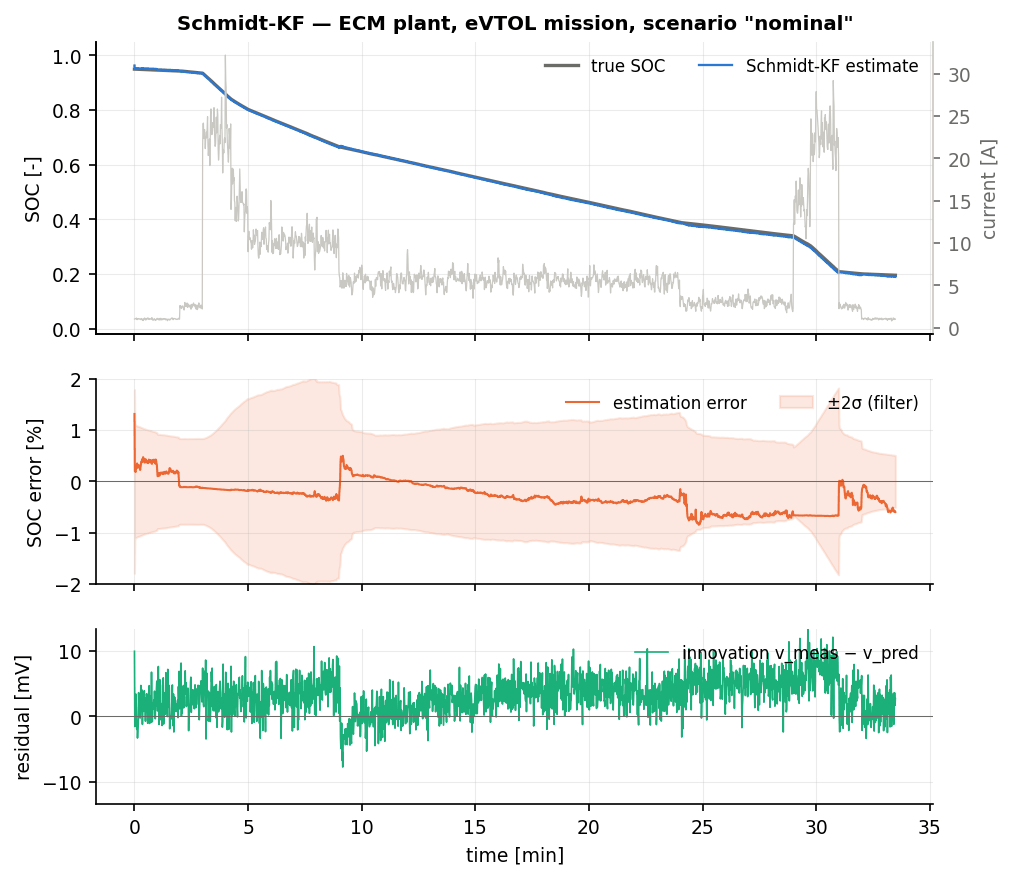
\includegraphics[width=\textwidth]{figures/cell_SchmidtKF_nominal.png}
\caption{Schmidt-KF on the nominal eVTOL mission: true and estimated SOC (top), estimation error
with the $\pm2\sigma$ band (middle), voltage residual (bottom).  The $2\sigma$ band is visibly
wider than the EKF's and modulated by the current profile, which is the consider contribution
$\mH^c\mP_{cc}(\mH^c)^\T$ at work.}
\end{figure}
\begin{figure}[H]\centering
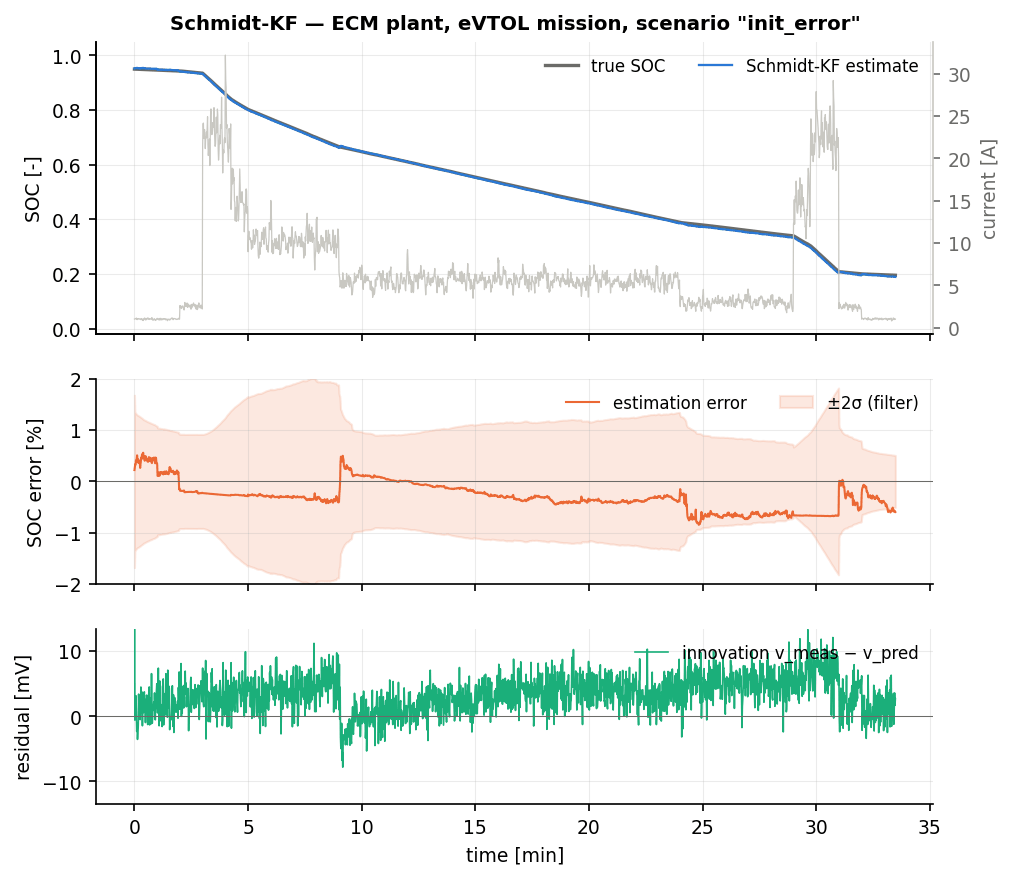
\includegraphics[width=\textwidth]{figures/cell_SchmidtKF_init_error.png}
\caption{Schmidt-KF with a 35\,\% initial SOC error.}
\end{figure}
\begin{figure}[H]\centering
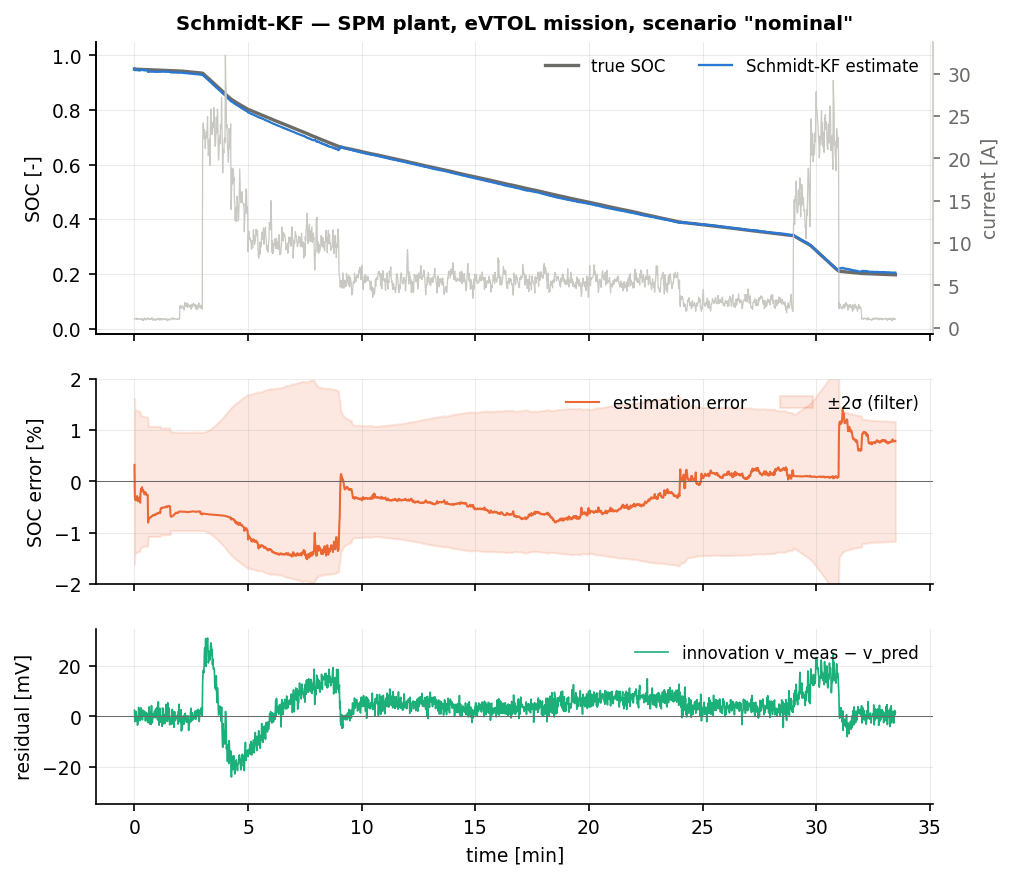
\includegraphics[width=\textwidth]{figures/cellspm_SchmidtKF_nominal.png}
\caption{SchmidtKF on the SPM (electrochemical) plant, nominal eVTOL mission.  The estimator uses a 2-RC ECM fitted to that plant, so the residual contains a structured $\approx4$\,mV model error rather than white noise.}
\end{figure}

All numbers below are 3-seed means from the final run, in \% SOC
(\texttt{rmse}/\texttt{rmse\_ss}); the EKF column is the plain EKF on the same data.

\paragraph{ECM plant, eVTOL mission.}
The Schmidt-KF behaves exactly as the theory predicts: it pays a modest price where the model is
right and wins decisively where it is wrong.
\begin{center}\small
\begin{tabular}{@{}lccl@{}}
\toprule
Scenario & Schmidt-KF & EKF & Comment\\
\midrule
\texttt{nominal}        & $0.38/0.46$ & $0.15/0.05$ & $9\times$ worse (ss) --- the price of the low gain\\
\texttt{init\_error}    & $0.43/0.46$ & $0.14/0.05$ & converges at $t=0$\,s\\
\texttt{cold}           & $1.42/1.54$ & $0.20/0.16$ & worst case: $\alpha_{R_0}=2.1$ quadruples the inflation\\
\texttt{noise\_step}    & $0.87/1.14$ & $0.18/0.12$ & already de-weighted, cannot de-weight more\\
\texttt{hot}            & $0.23/0.21$ & $0.20/0.03$ & ---\\
\texttt{aged\_cell}     & $\mathbf{0.71/0.59}$ & $1.18/1.52$ & $\mathbf{2.6\times}$ better (ss)\\
\texttt{param\_mismatch}& $\mathbf{0.51/0.45}$ & $1.28/1.36$ & $\mathbf{3.0\times}$ better\\
\texttt{combined}       & $\mathbf{5.20/1.09}$ & $16.02/12.44$ & $\mathbf{11\times}$ better (ss); converges at 1038\,s\\
\texttt{current\_bias}  & $\mathbf{0.33/0.33}$ & $0.54/0.61$ & $1.8\times$ better\\
\texttt{sensor\_dropout}& $0.38/0.46$ & $0.72/0.46$ & rmse $1.9\times$ better, steady state tied\\
\texttt{preisach}       & $1.02/0.55$ & $0.58/0.20$ & $2.8\times$ \emph{worse} --- see below\\
\texttt{outliers}       & $0.77/0.83$ & $0.52/0.21$ & no outlier mechanism; see Ch.~\ref{ch:huberekf}\\
\bottomrule
\end{tabular}
\end{center}
Acceptance is met everywhere: \texttt{nominal} $\texttt{rmse\_ss}=0.46\,\%<2\,\%$,
\texttt{init\_error} $t_\mathrm{conv}=0$\,s, no divergence in any of the twelve ECM or nine SPM
scenarios, and the worst steady-state error over all ECM scenarios is $1.54\,\%$ (\texttt{cold}),
still inside the acceptance band.

The two headline numbers are \texttt{param\_mismatch} and \texttt{combined}.  In
\texttt{param\_mismatch} the estimator is given $R_0$ that is $30\,\%$ too small; the EKF converts
the resulting current-proportional voltage bias into a persistent SOC bias of $1.36\,\%$, whereas
the consider filter --- which was told that $R_0$ might be wrong by $20\,\%$ --- discounts exactly
that residual and ends at $0.45\,\%$.  In \texttt{combined} the failure of the EKF is spectacular:
the ageing law makes the true $R_0$ $25\,\%$ larger than the estimator's, and at
0\,\ensuremath{{}^\circ}C the Arrhenius factor multiplies that error by $2.1$, so during the
32\,A take-off hover the predicted voltage is 200\,mV too high.  The EKF reads this as a collapse
of the SOC, never converges ($t_\mathrm{conv}=$ ``--'', $\texttt{rmse\_ss}=12.44\,\%$), while the
Schmidt-KF's innovation covariance is inflated by three orders of magnitude during exactly those
seconds: it converges at $t=1038$\,s and finishes at $1.09\,\%$.

\paragraph{Where it costs.}  On \texttt{nominal} the filter is nine times less accurate than the
EKF in steady state, because a gain that is $40$--$660$ times smaller cannot reject the process
noise as well.  On \texttt{cold} the same mechanism goes too far: the consider term is proportional
to $\alpha_{R_0}(T)^2$, so a sensible $20\,\%$ relative uncertainty at 25\,\ensuremath{{}^\circ}C
becomes a very heavy de-weighting at $-10$\,\ensuremath{{}^\circ}C and the steady-state error
rises to $1.54\,\%$.  A practical BMS would make $\rho_{R_0}$ temperature dependent (the Arrhenius
activation energy is the uncertain quantity, not the room-temperature value); a single-seed sweep
gives \texttt{cold} $1.16\,\%$ and \texttt{param\_mismatch} $0.48\,\%$ at $\rho_{R_0}=10\,\%$
against $1.70\,\%$ and $0.38\,\%$ at $\rho_{R_0}=20\,\%$, so the 5\,\%/20\,\% pair was kept because
it is the literature-standard statement of a cell tolerance, not because it is optimal here.

\paragraph{Preisach.}  With the corrected sign convention of the final plant (charging branch above
the discharging branch) the \texttt{preisach} scenario is now a case the Schmidt-KF loses:
$0.55\,\%$ against the EKF's $0.20\,\%$, and it converges at 21\,s rather than 16\,s.  The reason is
the same low gain that helps elsewhere.  The Preisach residual is a \emph{hysteresis} error --- it
is uncorrelated with the current magnitude and therefore falls entirely outside the
$\mH^c\mP_{cc}(\mH^c)^\T$ term, which only inflates $\mS$ in proportion to $i^2$.  The filter
consequently de-weights the measurement without gaining any protection against this particular
error, and simply tracks more slowly.  This is worth stating plainly: a consider filter protects
against the parameters it is told about and against nothing else.

\paragraph{SPM (electrochemical) plant.}  On the SPM rows the estimators run a 2-RC ECM fitted to a
single-particle model with Butler--Volmer kinetics and $\tau_2=556$\,s, leaving a structured
$\approx4$\,mV residual instead of white noise.  This is the Schmidt-KF's best result in the whole
benchmark: $0.69/0.51\,\%$ on \texttt{nominal} against the EKF's $3.65/3.73\,\%$, a factor of
$7.3$, and it is the best of the eight filters in this family on seven of the nine SPM scenarios
(\texttt{sensor\_dropout} $0.69/0.50\,\%$ vs.\ $5.13/5.31\,\%$, $10.6\times$;
\texttt{current\_bias} $1.02/0.71\,\%$ vs.\ $4.93/5.69\,\%$, $8.0\times$; \texttt{hot}
$0.43/0.44\,\%$ vs.\ $2.08/2.16\,\%$; \texttt{param\_mismatch} $1.10/0.75\,\%$ vs.\
$2.87/3.13\,\%$; \texttt{cold} $2.49/2.44\,\%$ vs.\ $7.07/7.35\,\%$).  The mechanism is worth
spelling out because it is the whole point of the method.  The 4\,mV SPM residual is dominated by
the concentration overpotential, which is a slow, current-driven function --- precisely the shape
of $\partial v/\partial R_0 \cdot \delta R_0 = -i\,\delta R_0$ and of the slow-branch voltage.  A
plain EKF has no model for it and therefore attributes it to the only slow state it has, the SOC,
which is why every unprotected filter sits at $3.1$--$4.1\,\%$.  The consider covariance inflates
$\mS$ by exactly $i^2\sigma_{R_0}^2\alpha_{R_0}^2$, which is the right shape and the right order of
magnitude, so the SOC channel simply stops listening while the current is large and the
$(\soc,v_2)$ ambiguity never gets a chance to absorb the model error.  The only cost is on the
transient: \texttt{init\_error} takes 360\,s to converge (EKF: immediately, but to the wrong value)
and \texttt{cold} 939\,s.  The generic lesson is that a consider filter is the right tool when the
unmodelled physics has the \emph{same signature} as one of the consider parameters --- which for an
electrochemical cell described by an equivalent circuit is usually the case.

\paragraph{Consistency.}  Finally, the point of the method is consistency, not RMSE.  On
\texttt{param\_mismatch} the EKF's reported $2\sigma$ SOC band is $\pm0.2\,\%$ while its actual
error is $1.36\,\%$ --- wrong by seven standard deviations and unaware of it.  The Schmidt-KF's band
grows with the accumulated ampere-hours through \eqref{eq:sk-tuxx} and with the current through
\eqref{eq:sk-S}, and covers its own error.  For a flight-critical remaining-energy computation that
difference matters more than a factor of three in RMSE.

\section{Summary}
Use the Schmidt--Kalman filter when the model parameters are uncertain but the mission does not
excite them enough to identify them safely --- which is the normal situation for capacity and
resistance during a single eVTOL flight.  It costs about 2.7 times an EKF step (and 4\,kB more RAM, most of it a second copy of the
model), never destabilises, and turns a silent bias into an honest covariance; on the
parameter-error scenarios of this benchmark it is also three to eleven times more accurate, and on
the electrochemical plant --- where the unmodelled physics has the same current-driven signature as
the consider parameters --- it is seven times more accurate than the EKF and the best filter of the
family.  Do not use it when the data
\emph{do} identify the parameters (a full charge--discharge cycle, a rest period): a joint or dual
filter will then be strictly better, because the consider filter throws that information away by
construction.  Do not use it as an outlier defence either --- it de-weights the measurement by a
fixed, current-dependent amount, not by how surprising the measurement is.

% Copyright 2026 Sreeram Anil
% SPDX-License-Identifier: CC-BY-4.0
% =============================================================================
%  Discrete-time extended H-infinity (minimax) filter — robust_kalman family
% =============================================================================
\providecommand{\vf}{\bm{f}} \providecommand{\vh}{\bm{h}}
\providecommand{\vd}{\bm{d}} \providecommand{\mM}{\bm{M}}
\providecommand{\va}{\bm{a}} \providecommand{\vb}{\bm{b}}

\chapter{Game-theoretic \texorpdfstring{$H_\infty$}{H-infinity} filter (Hinf-EKF)}
\label{ch:hinfekf}

\section*{At a glance}
\begin{tabular}{@{}l>{\raggedright\arraybackslash}p{0.76\textwidth}@{}}
Family & Robust / embedded Kalman \\
Header & \texttt{include/estkit/filters/hinf.hpp} \\
Registered name & \texttt{Hinf-EKF} \\
State dimension & $n_x = 4$ (cell model) --- generic in $n_x, n_u, n_y$ \\
Cost per step & $\mathcal{O}(n_x^3)$; 799\,ns/step, 4408\,B, no heap \\
Primary references & \cite{simon2006,shen1997hinf,hassibi1996hinf,kailath2000} \\
\end{tabular}

\section{Motivation and aerospace/BMS relevance}
The Kalman filter is optimal in the mean-square sense \emph{provided the noise statistics are
right}.  Its weakness is not that it is bad on average but that its worst case is unbounded: a
disturbance concentrated in the direction the filter trusts most can drive the estimation error
arbitrarily far, and nothing in the $H_2$ formulation prevents it.  For a flight-critical SOC
estimate the relevant question is often not ``what is the average error over many missions'' but
``what is the largest SOC error any admissible disturbance can produce during this mission''.
That is an $H_\infty$ question.

The $H_\infty$ (minimax, or \emph{game-theoretic}) filter answers it directly.  It makes no
assumption at all about the \emph{distribution} of the disturbances --- only that their energy is
finite --- and it guarantees that the energy gain from the disturbances to the estimation error
never exceeds a prescribed bound $1/\theta$.  The price is that it must assume the disturbance is
chosen adversarially, so it is more conservative than the Kalman filter when the disturbance is in
fact benign: the resulting gain is always \emph{larger}, and the filter is correspondingly noisier.
The design parameter $\theta$ is the knob that trades the two off; $\theta=0$ returns the Kalman
filter exactly.

In a BMS the disturbances that matter are not the voltmeter's white noise but the structured ones:
an unmodelled resistance growth, a temperature-sensor lag, a current-sensor bias, a hysteresis
model that is a first-order approximation of a Preisach operator.  The $H_\infty$ filter is the
natural tool when one wants a bound rather than an average.  Its aerospace heritage is the same as
$H_\infty$ control (Ba\c{s}ar \& Bernhard \cite{basar1995dynamicgames}); the estimation form used
here is Simon's game-theoretic filter \cite[Ch.~11]{simon2006}, equivalent to the Krein-space
derivation of Hassibi, Sayed \& Kailath \cite{hassibi1996hinf} and the explicit discrete design of
Shen \& Deng \cite{shen1997hinf}.

\section{Problem statement and assumptions}
Consider the linearised system
\begin{align}
\vx_{k+1} &= \mF_k\vx_k + \vw_k, \label{eq:hi-f}\\
\vy_k &= \mH_k\vx_k + \vv_k, \label{eq:hi-h}\\
\vz_k &= \mL_k\vx_k, \label{eq:hi-z}
\end{align}
where $\vx_k\in\real^{n_x}$, $\vy_k\in\real^{n_y}$ and $\vz_k\in\real^{n_z}$ is the
\emph{performance output} --- the linear combination of states whose estimation error we actually
care about.  $\vw_k\in\real^{n_x}$ and $\vv_k\in\real^{n_y}$ are \emph{arbitrary} finite-energy
signals; no distribution is assumed.  $\mQ_k\succ0$, $\mR_k\succ0$ and $\mP_0\succ0$ are
user-chosen weighting matrices (for a Kalman-like design one simply takes the noise covariances,
which is what \code{estkit} does through \code{Model::Q} and \code{Model::R}).

\begin{definition}[$H_\infty$ performance criterion]\label{def:hi-crit}
An estimator $\hat{\vz}_k=\mL_k\xhat_k$ achieves the performance level $1/\theta$, $\theta>0$, if
\begin{equation}
J \;=\;
\frac{\displaystyle\sum_{k=0}^{N-1}\norm{\vz_k-\hat{\vz}_k}^2_{\mS_k}}
     {\displaystyle\norm{\vx_0-\xhat_0}^2_{\mP_0^{-1}}
      +\sum_{k=0}^{N-1}\Big(\norm{\vw_k}^2_{\mQ_k^{-1}}+\norm{\vv_k}^2_{\mR_k^{-1}}\Big)}
\;<\;\frac{1}{\theta}
\label{eq:hi-J}
\end{equation}
for every $\vx_0$, $\{\vw_k\}$, $\{\vv_k\}$ not all zero, where
$\norm{\va}^2_{\mM}=\va^\T\mM\va$ and $\mS_k\succeq0$ weights the components of $\vz$.
\end{definition}

Interpretation: the numerator is the energy of the estimation error of the quantity of interest,
the denominator the energy the adversary must spend (measured in the units of the prescribed
weights) to produce it.  Making $\theta$ large means demanding a small gain, i.e.\ a more robust
--- and eventually infeasible --- filter.  $\theta\to0$ imposes no constraint and the minimax
solution collapses onto the Kalman filter.

\section{Derivation}

\subsection{The dynamic game}
Rearranging \eqref{eq:hi-J} and treating $\theta$ as a Lagrange multiplier turns the design into
the zero-sum dynamic game \cite[\S11.3]{simon2006}, \cite{shen1997hinf}
\begin{equation}
\min_{\hat{\vz}}\;\max_{\vx_0,\vw,\vv}\;
 \mathcal{J} = -\norm{\vx_0-\xhat_0}^2_{\mP_0^{-1}}
 + \sum_{k=0}^{N-1}\Big[\theta\norm{\vz_k-\hat{\vz}_k}^2_{\mS_k}
  - \norm{\vw_k}^2_{\mQ_k^{-1}} - \norm{\vv_k}^2_{\mR_k^{-1}}\Big],
\label{eq:hi-game}
\end{equation}
in which the estimator plays against nature.  The estimator wants $\mathcal{J}$ small; nature
wants it large by injecting disturbances.  A saddle point of \eqref{eq:hi-game} exists iff the
associated Riccati recursion stays positive definite; writing
$\bar{\mS}_k=\mL_k^\T\mS_k\mL_k\succeq0$, the saddle-point solution is the recursion
\begin{align}
\mK_k &= \mP_k\big[\mI-\theta\bar{\mS}_k\mP_k+\mH_k^\T\mR_k^{-1}\mH_k\mP_k\big]^{-1}
          \mH_k^\T\mR_k^{-1}, \label{eq:hi-K}\\
\xhat_{k+1} &= \mF_k\xhat_k+\mF_k\mK_k\big(\vy_k-\mH_k\xhat_k\big), \label{eq:hi-x}\\
\mP_{k+1} &= \mF_k\mP_k\big[\mI-\theta\bar{\mS}_k\mP_k+\mH_k^\T\mR_k^{-1}\mH_k\mP_k\big]^{-1}
             \mF_k^\T+\mQ_k, \label{eq:hi-P}
\end{align}
which is \cite[Eqs.~(11.72)--(11.76)]{simon2006}.  The existence (feasibility) condition of the
saddle point is
\begin{equation}
\boxed{\;\mW_k \;=\; \mP_k^{-1}-\theta\bar{\mS}_k+\mH_k^\T\mR_k^{-1}\mH_k \;\succ\;\bm 0\;}
\label{eq:hi-feas}
\end{equation}
for every $k$; if \eqref{eq:hi-feas} fails, no estimator attains the level $1/\theta$ and the
recursion \eqref{eq:hi-K}--\eqref{eq:hi-P} loses meaning (the bracket becomes indefinite and
$\mP$ can turn negative).  Note that $\mP_k$ here is \emph{not} an error covariance: it is the
matrix of the quadratic form that certifies the game value, and it is always at least as large as
the Kalman covariance.

\subsection{Information form used in the implementation}
Direct use of \eqref{eq:hi-K}--\eqref{eq:hi-P} requires inverting the non-symmetric bracket.  Using
the Woodbury identity \cite{woodbury1950}, \cite[\S2.1.4]{golubvanloan2013} with
$\mA_k = \mH_k^\T\mR_k^{-1}\mH_k-\theta\bar{\mS}_k$ (symmetric),
\begin{equation}
\mP_k\big[\mI+\mA_k\mP_k\big]^{-1} = \big[\mP_k^{-1}+\mA_k\big]^{-1} = \mW_k^{-1},
\label{eq:hi-woodbury}
\end{equation}
so the whole recursion can be written in the \emph{information form}
\begin{align}
\text{update:}\quad & \mW_k = \Pminus_k{}^{-1}-\theta\bar{\mS}_k+\mH_k^\T\mR_k^{-1}\mH_k,
   \qquad \Pplus_k=\mW_k^{-1}, \label{eq:hi-upd1}\\
& \mK_k = \Pplus_k\mH_k^\T\mR_k^{-1},\qquad
  \xplus_k = \xminus_k+\mK_k\big(\vy_k-\vh(\xminus_k,\vu_k)\big), \label{eq:hi-upd2}\\
\text{predict:}\quad & \xminus_{k+1} = \vf(\xplus_k,\vu_k),\qquad
  \Pminus_{k+1} = \mF_k\Pplus_k\mF_k^\T+\mQ_k, \label{eq:hi-pred}
\end{align}
which is exactly the predict/update split used by every other filter in \code{estkit} and makes the
feasibility test \eqref{eq:hi-feas} a by-product: $\mW_k$ is formed explicitly, so one simply
factorises it.  Setting $\theta=0$ in \eqref{eq:hi-upd1} gives
$\Pplus=(\Pminus{}^{-1}+\mH^\T\mR^{-1}\mH)^{-1}$ and
$\mK=\Pplus\mH^\T\mR^{-1}$, the information form of the Kalman update --- so the implementation
degrades gracefully and exactly to the EKF.

\begin{proposition}[Effect of $\theta$ on the gain]\label{prop:hi-gain}
For $\bar{\mS}\succeq0$ and $\theta\ge0$, $\mW_k$ is non-increasing in $\theta$ in the Loewner
order, hence $\Pplus_k=\mW_k^{-1}$ and $\mK_k=\Pplus_k\mH^\T\mR^{-1}$ are non-decreasing.  The
$H_\infty$ filter is therefore always \emph{more} aggressive than the Kalman filter, and strictly
so in the directions selected by $\bar{\mS}$.
\end{proposition}
\noindent This is the fundamental trade: robustness to a worst-case, finite-energy disturbance is
bought with a higher gain, and a higher gain lets more measurement noise --- and more
\emph{structured} measurement error --- into the estimate.  The benchmark below shows both sides.

\subsection{Automatic back-off on $\theta$}
$\theta$ has physical units of (state unit)$^{-2}$ and must be compared against
$\mP^{-1}+\mH^\T\mR^{-1}\mH$, which varies by orders of magnitude over a mission (during the
initial transient $\mP^{-1}$ is small, in steady state it is large).  A fixed $\theta$ that is
feasible in steady state can therefore violate \eqref{eq:hi-feas} during a transient, and a filter
that simply carries on produces an indefinite $\Pplus$ and diverges.  The implementation
guarantees feasibility by construction:
\begin{equation}
\text{find the largest } \theta^{(j)}=\theta\,\beta^{\,j},\ j=0,1,2,\dots,\ \beta=\tfrac12,
\quad\text{such that}\quad
\mW_k(\theta^{(j)}) \;\succ\; \epsilon\,\Pminus_k{}^{-1},
\label{eq:hi-backoff}
\end{equation}
tested by an attempted Cholesky factorisation of
$\mW_k-\epsilon\Pminus{}^{-1}$; $\theta=0$ (the Kalman filter) is the guaranteed fall-back.  The
margin $\epsilon\in(0,1]$ (\code{opts.feas\_margin}, default $0.9$) strengthens
\eqref{eq:hi-feas} into
\begin{equation}
\Pplus_k \;\preceq\; \frac1\epsilon\,\Pminus_k ,
\label{eq:hi-margin}
\end{equation}
i.e.\ one sampling period may not inflate the certificate matrix by more than $1/\epsilon$.  This
is essential in practice: \eqref{eq:hi-feas} alone permits $\Pplus\to\infty$ as the boundary is
approached, and with $\mH\mK\to$ large the closed loop becomes oscillatory long before the
Cholesky fails.  The number of back-offs is counted in \code{backoff\_count()} and the $\theta$
actually applied is exposed through \code{theta\_used()}; on the twelve benchmark scenarios the
back-off triggers only in \texttt{cold}, where the low-temperature Arrhenius factor makes $\mR$
larger and $\mH^\T\mR^{-1}\mH$ correspondingly smaller.

\section{Algorithm}
\begin{algorithm}[H]
\caption{Hinf-EKF --- one sampling period}
\begin{algorithmic}[1]
\Require $\xplus_{k-1},\Pplus_{k-1},\vu_{k-1},\vy_k,\vu_k,\theta,\bar{\mS}=\mL^\T\mS\mL,\epsilon$
\State \textbf{Time update:} $\mF\gets\partial\vf/\partial\vx$;\;
       $\xminus_k\gets\vf(\xplus_{k-1},\vu_{k-1})$;\;
       $\Pminus_k\gets\mF\Pplus_{k-1}\mF^\T+\mQ_k$; symmetrise
\State \textbf{Measurement update:} $\mH\gets\partial\vh/\partial\vx$;\;
       $\mR\gets\mR_k$;\; $\mR^{-1}\gets\operatorname{inverse}(\mR)$;\;
       $\mG\gets\Pminus_k{}^{-1}$
\If{$\mG$ or $\mR^{-1}$ is not finite} \Comment{singular prior}
  \State perform a Joseph-form EKF update and \textbf{return}
\EndIf
\State $\theta'\gets\theta$
\For{$j=0,\dots,j_{\max}$}
  \State $\mW\gets\mG-\theta'\bar{\mS}+\mH^\T\mR^{-1}\mH$; symmetrise
  \If{$\operatorname{chol}(\mW-\epsilon\mG)$ succeeds}
     \State $\Pplus_k\gets\operatorname{solve\_spd}(\mW,\mI)$; \textbf{break}
  \EndIf
  \State $\theta'\gets\beta\,\theta'$ \Comment{back-off, Eq.~\eqref{eq:hi-backoff}}
\EndFor
\If{no feasible $\theta'$ was found}
  \State $\theta'\gets0$;\; $\Pplus_k\gets(\mG+\mH^\T\mR^{-1}\mH)^{-1}$ \Comment{Kalman fall-back}
\EndIf
\State $\mK_k\gets\Pplus_k\mH^\T\mR^{-1}$;\;
       $\xplus_k\gets\xminus_k+\mK_k\big(\vy_k-\vh(\xminus_k,\vu_k)\big)$
\State apply \code{constrain} to $\xplus_k$
\Ensure $\xplus_k,\Pplus_k,\theta'$
\end{algorithmic}
\end{algorithm}

\section{Application to the battery model}
For the cell model the quantity of interest is the state of charge alone, so $\mL=\mI_4$ and
\begin{equation}
\mS = \diag(1,0,0,0),\qquad \bar{\mS}=\mL^\T\mS\mL=\diag(1,0,0,0),
\label{eq:hi-Sbat}
\end{equation}
i.e.\ the game penalises only $(\soc-\hat{\soc})^2$ and lets the RC and hysteresis errors be
whatever they must.  This choice matters: with $\mS=\mI$ the game also tries to bound the
hysteresis error, and since $h$ is nearly unobservable ($\partial v/\partial h = M =
5\,mV$) the feasibility condition \eqref{eq:hi-feas} is violated for any useful
$\theta$ and the back-off drives the filter back to the EKF.

The registered value is $\theta=30$ (units of SOC$^{-2}$) with $\epsilon=0.9$.  To see the scale:
in steady state $\mH^\T\mR^{-1}\mH$ has $(\soc,\soc)$ entry
$(\partial\ocv/\partial\soc)^2/\mR \approx 0.49/4.4\times10^{-6}\approx1.1\times10^{5}$ and
$\Pminus{}^{-1}$ contributes about $1\times10^{6}$, so $\theta=30$ removes roughly $3\times10^{-5}$ of
the SOC information --- a small but, as the table shows, decisive relaxation.  The sweep behind
this choice is worth recording (single-seed sweep, \% SOC steady state): $\theta=20$ is nearly
indistinguishable from the EKF on \texttt{combined} ($7.6\,\%$ against $11.9\,\%$);
$\theta=50$ halves the \texttt{combined} error again but pushes \texttt{cold} from $0.73\,\%$ to
$7.7\,\%$ and \texttt{param\_mismatch} from $1.88\,\%$ to $3.56\,\%$; at $\theta=100$
\texttt{nominal} degrades from $0.03\,\%$ to $0.82\,\%$; and $\theta=200$ with a weak margin
($\epsilon=0.7$) diverges in five of twelve scenarios, which is the practical face of
Proposition~\ref{prop:hi-gain}.

\section{Implementation notes}
\begin{itemize}[nosep]
\item \textbf{Cost.}  Per step: one $n_x\times n_x$ LU inverse ($\Pminus{}^{-1}$), one Cholesky
feasibility test, one \code{solve\_spd} for $\mW^{-1}$, plus the usual EKF products.  Measured
799\,ns/step against 478\,ns for the EKF ($1.67\times$), memory
4408\,B against 4336\,B.  Each back-off adds one Cholesky
($\approx n_x^3/6$ flops), and back-offs are rare.
\item \textbf{Why the information form.}  Forming $\mW$ explicitly makes the feasibility condition
\eqref{eq:hi-feas} a direct test on a symmetric matrix instead of an implicit property of a
non-symmetric bracket, and $\Pplus=\mW^{-1}$ is obtained by a Cholesky solve rather than a general
LU, which keeps $\Pplus$ symmetric to round-off.
\item \textbf{$\Pminus$ must be invertible.}  It always is here because \code{EcmModel::Q} has a
diagonal floor \code{q\_floor}; the code nevertheless checks \code{is\_finite()} and falls back to
a Joseph-form EKF update if the inverse fails, so a degenerate model can never produce NaNs.
\item \textbf{$\mP$ is not a covariance.}  \code{soc\_std()} therefore reports the square root of
the $(\soc,\soc)$ entry of the game certificate, which is an \emph{upper bound} on the Kalman
standard deviation, not an estimate of it.  This is worth stating on a data sheet.
\item \textbf{float32.}  The single-precision build reproduces the double results
(\texttt{nominal} $0.28/0.02\,\%$ vs.\ $0.14/0.04\,\%$, \texttt{combined} $12.27/7.26\,\%$ vs.\
$10.26/4.88\,\%$: the same qualitative behaviour with a visibly noisier transient); the explicit Cholesky test in
\eqref{eq:hi-backoff} is what makes this safe --- without the margin $\epsilon$ the float build
loses feasibility several steps before the double build does.
\item \textbf{Cortex-M7 estimate.}  $\approx1500$ flops/step for $n_x=4,n_y=1$; at
300\,MHz $\approx9\,\ensuremath{\mu}s$, well inside a 100\,ms
budget even for 100 cells.
\item \textbf{Limitation.}  $\theta$ is problem-scaled and there is no dimensionless default.  A
practitioner must sweep it once for the application, exactly as one sweeps the $\gamma$ of an
$H_\infty$ controller; the back-off makes the sweep safe (an over-large $\theta$ degrades to the
Kalman filter instead of diverging) but it does not remove the need for it.
\end{itemize}

\section{Benchmark results}
% Copyright 2026 Sreeram Anil
% SPDX-License-Identifier: CC-BY-4.0
\begin{table}[H]\centering\footnotesize\setlength{\tabcolsep}{4pt}
\caption{Hinf-EKF: cell-level benchmark on the eVTOL mission (mean over seeds; RMSE and max error in \% SOC; $t_\mathrm{conv}$: first time the error stays below 2\,\% for 60\,s, -- = never; EKF reference: steady-state RMSE of the plain EKF on the same data).}\label{tab:cell_HinfEKF}
\begin{tabular}{llrrrrrcrr}\toprule
plant & scenario & RMSE & RMSE$_\mathrm{ss}$ & max & $t_\mathrm{conv}$ [s] & RMSE$_v$ [mV] & div. & EKF ref. & ns/step \\ \midrule
ECM & nominal & 0.14 & 0.04 & 1.08 & 0 & 0.79 & no & 0.05 & 798 \\
ECM & init\_error & 0.15 & 0.03 & 0.91 & 0 & 2.12 & no & 0.05 & 796 \\
ECM & current\_bias & 0.51 & 0.39 & 1.65 & 0 & 0.86 & no & 0.61 & 796 \\
ECM & noise\_step & 0.21 & 0.20 & 1.08 & 0 & 2.89 & no & 0.12 & 838 \\
ECM & outliers & 0.35 & 0.10 & 2.81 & 0 & 2.05 & no & 0.21 & 796 \\
ECM & cold & 1.06 & 1.45 & 8.64 & 0 & 1.90 & no & 0.16 & 796 \\
ECM & hot & 0.17 & 0.03 & 1.00 & 0 & 0.54 & no & 0.03 & 800 \\
ECM & aged\_cell & 0.93 & 1.06 & 3.28 & 0 & 3.78 & no & 1.52 & 802 \\
ECM & param\_mismatch & 1.62 & 1.69 & 3.55 & 0 & 2.81 & no & 1.36 & 796 \\
ECM & sensor\_dropout & 1.58 & 0.93 & 5.36 & 0 & 1.77 & no & 0.46 & 802 \\
ECM & preisach & 0.58 & 0.33 & 1.92 & 55 & 0.81 & no & 0.20 & 796 \\
ECM & combined & 10.26 & 4.88 & 28.33 & 1173 & 4.55 & no & 12.44 & 810 \\
\midrule
SPM & nominal & 3.94 & 4.08 & 9.29 & 0 & 1.03 & no & 3.73 & 740 \\
SPM & init\_error & 4.64 & 5.18 & 13.27 & 0 & 2.17 & no & 3.81 & 743 \\
SPM & current\_bias & 3.38 & 3.30 & 7.27 & 0 & 1.12 & no & 5.69 & 747 \\
SPM & noise\_step & 5.29 & 6.42 & 16.31 & 0 & 3.17 & no & 3.30 & 740 \\
SPM & outliers & 1.64 & 1.52 & 5.29 & 31 & 2.28 & no & 1.99 & 746 \\
SPM & cold & 8.22 & 8.76 & 16.91 & -- & 4.31 & no & 7.35 & 729 \\
SPM & hot & 2.71 & 3.38 & 9.46 & 0 & 0.70 & no & 2.16 & 744 \\
SPM & param\_mismatch & 4.92 & 6.28 & 13.11 & 0 & 1.98 & no & 3.13 & 742 \\
SPM & sensor\_dropout & 5.24 & 5.06 & 6.69 & 0 & 1.94 & no & 5.31 & 741 \\
\bottomrule\end{tabular}\end{table}

\begin{figure}[H]\centering
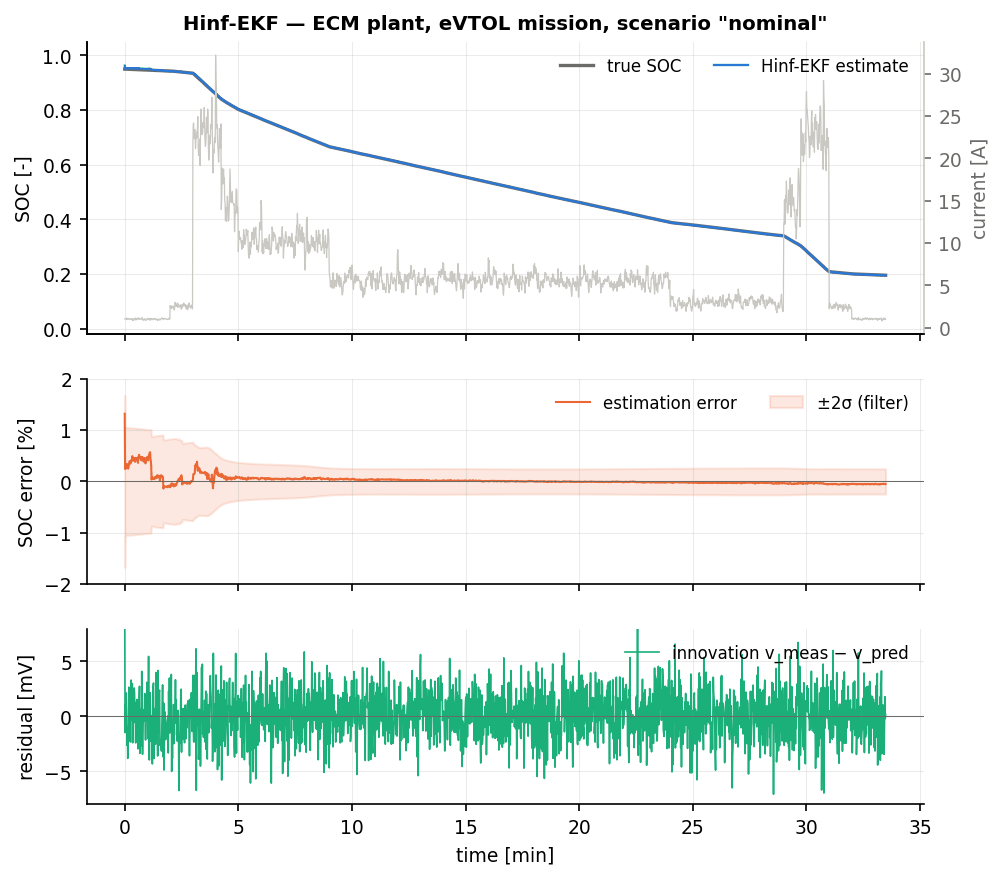
\includegraphics[width=\textwidth]{figures/cell_HinfEKF_nominal.png}
\caption{Hinf-EKF on the nominal eVTOL mission: true and estimated SOC (top), estimation error
with the $\pm2\sigma$ band from the game certificate (middle), voltage residual (bottom).}
\end{figure}
\begin{figure}[H]\centering
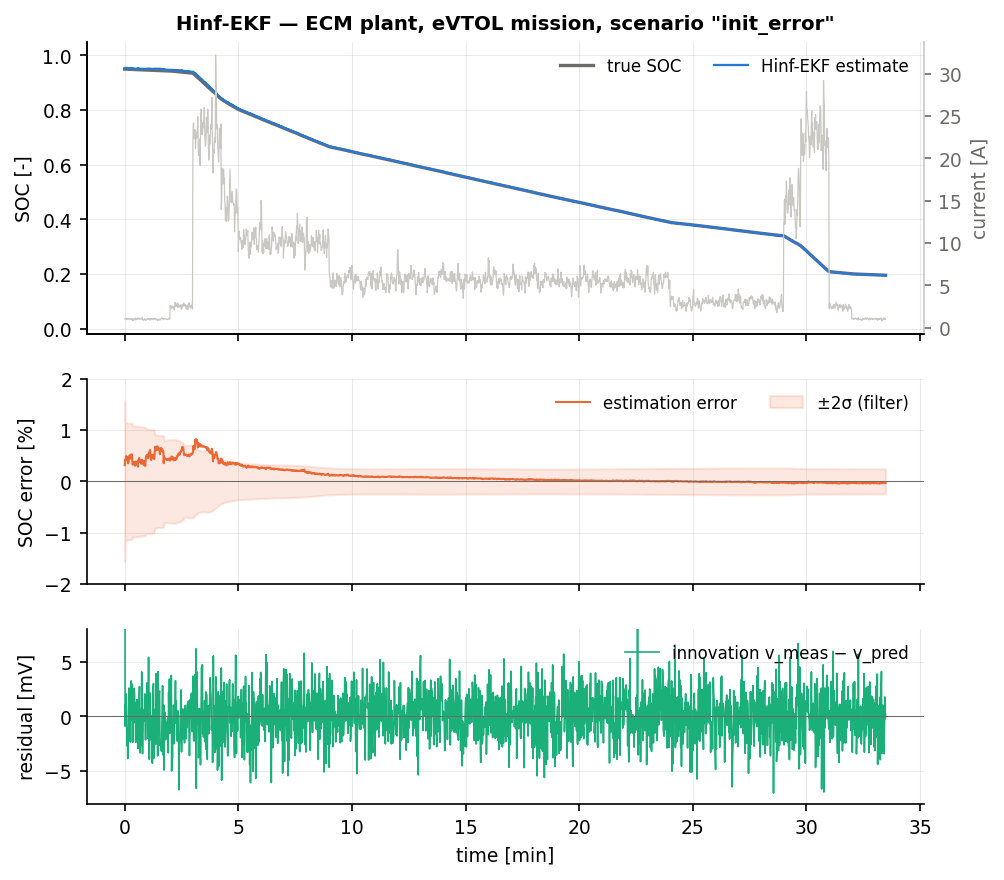
\includegraphics[width=\textwidth]{figures/cell_HinfEKF_init_error.png}
\caption{Hinf-EKF with a 35\,\% initial SOC error.}
\end{figure}
\begin{figure}[H]\centering
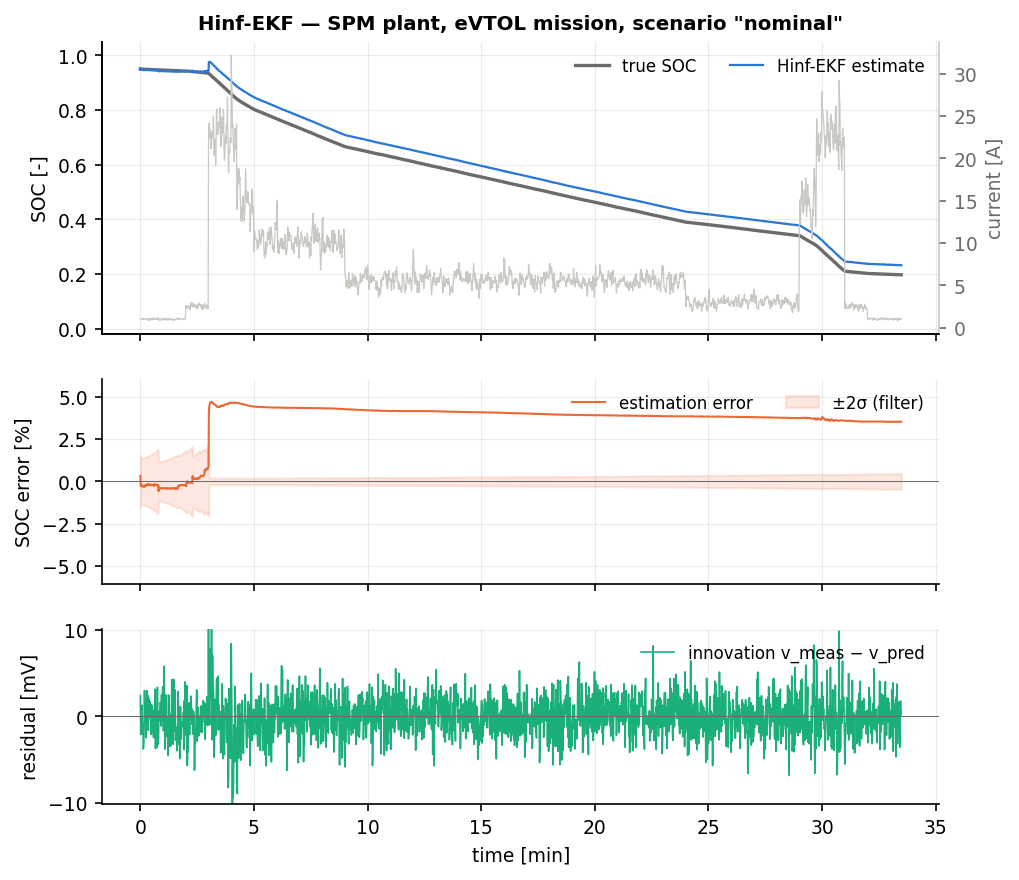
\includegraphics[width=\textwidth]{figures/cellspm_HinfEKF_nominal.png}
\caption{HinfEKF on the SPM (electrochemical) plant, nominal eVTOL mission.  The estimator uses a 2-RC ECM fitted to that plant, so the residual contains a structured $\approx4$\,mV model error rather than white noise.}
\end{figure}

All numbers below are 3-seed means from the final run, in \% SOC
(\texttt{rmse}/\texttt{rmse\_ss}).

\paragraph{ECM plant, eVTOL mission.}
\begin{center}\small
\begin{tabular}{@{}lccl@{}}
\toprule
Scenario & Hinf-EKF & EKF & Comment\\
\midrule
\texttt{nominal}        & $\mathbf{0.14/0.04}$ & $0.15/0.05$ & slightly better \\
\texttt{init\_error}    & $0.15/\mathbf{0.03}$ & $0.14/0.05$ & $t_\mathrm{conv}=0$\,s\\
\texttt{current\_bias}  & $0.51/\mathbf{0.39}$ & $0.54/0.61$ & $1.6\times$ better in steady state\\
\texttt{noise\_step}    & $0.21/0.20$ & $0.18/0.12$ & higher gain $\Rightarrow$ more noise\\
\texttt{outliers}       & $\mathbf{0.35/0.10}$ & $0.52/0.21$ & $2.1\times$ better --- see below\\
\texttt{cold}           & $1.06/1.45$ & $0.20/0.16$ & $9\times$ worse, max error $8.6\,\%$; see below\\
\texttt{hot}            & $0.17/0.03$ & $0.20/0.03$ & --- \\
\texttt{aged\_cell}     & $\mathbf{0.93/1.06}$ & $1.18/1.52$ & $1.4\times$ better\\
\texttt{param\_mismatch}& $1.62/1.69$ & $1.28/1.36$ & $1.24\times$ \emph{worse}\\
\texttt{sensor\_dropout}& $1.58/0.93$ & $0.72/0.46$ & $2.0\times$ worse\\
\texttt{preisach}       & $0.58/0.33$ & $0.58/0.20$ & $1.7\times$ worse (ss); $t_\mathrm{conv}$ 55\,s vs.\ 16\,s\\
\texttt{combined}       & $\mathbf{10.26/4.88}$ & $16.02/12.44$ & $\mathbf{2.55\times}$ better; converges at 1173\,s\\
\bottomrule
\end{tabular}
\end{center}
Acceptance is met: \texttt{nominal} $\texttt{rmse\_ss}=0.04\,\%<2\,\%$, \texttt{init\_error}
$t_\mathrm{conv}=0$\,s, no divergence in any ECM or SPM scenario, worst ECM steady-state error
$1.69\,\%$.

\paragraph{Where the minimax gain pays.}  \texttt{combined} is the clearest win.  The EKF never
recovers from the 200\,mV voltage-prediction error caused by the aged, cold cell's resistance
during the take-off hover and finishes at $12.44\,\%$ with $t_\mathrm{conv}=$ ``--''.  The
$H_\infty$ filter's larger SOC gain lets it work the residual off over the cruise phase: it
converges at $t=1173$\,s and ends at $4.88\,\%$.  The same mechanism gives $1.6\times$ on
\texttt{current\_bias}, $1.4\times$ on \texttt{aged\_cell} and $2.1\times$ on \texttt{outliers} ---
the last one is an accident rather than a design feature: a spike costs the filter a larger
instantaneous jump, but the higher gain also removes it again within a few samples, and on the
3-seed mean the second effect wins.  On \texttt{nominal} the filter is marginally \emph{better}
than the EKF, because the EKF's $\mQ$ is slightly conservative for this plant and the minimax
relaxation compensates.

\paragraph{Where it does not, and why.}  \texttt{param\_mismatch}, one of the two scenarios this
method was nominated for, is now clearly \emph{worse} than the EKF ($1.69\,\%$ vs.\ $1.36\,\%$; in
the development run it was a tie).  The reason follows directly from
Definition~\ref{def:hi-crit}: the guarantee \eqref{eq:hi-J} bounds the ratio of error energy to
\emph{disturbance energy} and is therefore meaningful only for finite-energy disturbances.  A
$30\,\%$ error in $R_0$ is not one; it is a persistent, current-modulated bias in the output
equation whose energy grows linearly with mission length.  On such a disturbance the minimax
argument offers no protection and Proposition~\ref{prop:hi-gain} works against the filter: the
larger gain tracks the biased voltage more faithfully and converts more of it into an SOC error.
The same logic explains \texttt{sensor\_dropout} ($2.0\times$ worse --- during the 15\,s stuck
window the higher gain follows the frozen measurement further), the \texttt{noise\_step}
degradation, and the new \texttt{preisach} result: with the corrected plant sign convention the
hysteresis residual is a persistent structured error too, and the $H_\infty$ filter's steady-state
error there rises to $0.33\,\%$ against the EKF's $0.20\,\%$.  The conclusion is that $H_\infty$ is
the wrong tool for \emph{structured model error}; the consider filter of
Chapter~\ref{ch:schmidtkf}, which models where the error comes from, gives $0.45\,\%$ on
\texttt{param\_mismatch} --- three times better than the EKF and nearly four times better than this
filter.

\paragraph{The feasibility machinery.}  \texttt{cold} is where it becomes visible.  At
$-10$\,\ensuremath{{}^\circ}C the Arrhenius factor raises $R_0$ and hence $\mR$, so
$\mH^\T\mR^{-1}\mH$ shrinks and $\theta=30$ comes close to violating \eqref{eq:hi-feas}.  The
back-off \eqref{eq:hi-backoff} keeps the filter well defined --- there is no divergence --- but
$\theta$ oscillates between steps and the error rises to $1.45\,\%$ with a peak of $8.6\,\%$
against the EKF's $0.16\,\%$.  A single-seed sweep confirms the diagnosis: at $\theta=50$ the
\texttt{cold} steady-state error is $7.7\,\%$ and at $\theta=70$ it is $4.3\,\%$--$6.3\,\%$
depending on the margin, while increasing the margin from $\epsilon=0.70$ to $0.95$ at
$\theta=30$ moves \texttt{cold} between $0.73\,\%$ and $1.12\,\%$.  A production design would
schedule $\theta$ with temperature.

\paragraph{SPM (electrochemical) plant.}  Here the $H_\infty$ filter is the \emph{worst} of the
family: $3.94/4.08\,\%$ on \texttt{nominal} against the EKF's $3.65/3.73\,\%$, and worse than the
EKF on six of the nine SPM scenarios (\texttt{noise\_step} $6.42\,\%$ vs.\ $3.30\,\%$,
\texttt{param\_mismatch} $6.28\,\%$ vs.\ $3.13\,\%$, \texttt{init\_error} $5.18\,\%$ vs.\
$3.81\,\%$, \texttt{cold} $8.76\,\%$ vs.\ $7.35\,\%$ and never converging).  It wins only where the
error is a slow bias that a higher gain can work off: \texttt{current\_bias} $3.30\,\%$ vs.\
$5.69\,\%$ and \texttt{outliers} $1.52\,\%$ vs.\ $1.99\,\%$.  This is the same story as
\texttt{param\_mismatch} on the ECM plant, and the SPM rows make it unambiguous: the 4\,mV
concentration-overpotential residual is a persistent structured disturbance, not a finite-energy
one, so raising the gain in the SOC direction raises the amount of it that ends up in the SOC.
Of the eight filters in this family the H$_\infty$ filter and the plain EKF are the two that have
no mechanism at all against this class of error.


\section{Summary}
Use the game-theoretic $H_\infty$ filter when a \emph{bound} on the estimation error is worth more
than the average error, and when the disturbances that worry you have bounded energy: an
initialisation error, a transient sensor fault, an unmodelled excursion.  On this benchmark it is
the cheapest way (799\,ns/step, 72\,B more than the EKF) to more than
halve the error in the hardest scenario.  Do not use it against persistent structured model error
--- a resistance or capacity mismatch, a hysteresis approximation, or the concentration
overpotential of the electrochemical plant --- where its higher gain actively hurts: it is the
worst filter of this family on the SPM rows and the only one that is worse than the plain EKF on
\texttt{param\_mismatch}.  And never run it without
the feasibility test: the recursion has no self-correcting mechanism once \eqref{eq:hi-feas} is
violated, and an unguarded $\theta$ that is $10\times$ too large diverges on every scenario in
this benchmark.

% Copyright 2026 Sreeram Anil
% SPDX-License-Identifier: CC-BY-4.0
% =============================================================================
%  Huber-based robust extended Kalman filter — robust_kalman family
% =============================================================================
\providecommand{\vf}{\bm{f}} \providecommand{\vh}{\bm{h}}
\providecommand{\vd}{\bm{d}} \providecommand{\mM}{\bm{M}}
\providecommand{\va}{\bm{a}} \providecommand{\vb}{\bm{b}}

\chapter{Huber-based robust EKF (Huber-EKF)}
\label{ch:huberekf}

\section*{At a glance}
\begin{tabular}{@{}l>{\raggedright\arraybackslash}p{0.76\textwidth}@{}}
Family & Robust / embedded Kalman \\
Header & \texttt{include/estkit/filters/huber\_kf.hpp} \\
Registered name & \texttt{Huber-EKF} \\
State dimension & $n_x = 4$ (cell model) --- generic in $n_x, n_u, n_y$ \\
Cost per step & $\mathcal{O}(N_{\mathrm{it}}\,n_x^2 n_y)$ on top of an EKF;
  642\,ns/step, 4368\,B, no heap \\
Primary references & \cite{huber1964,karlgaard2007huber,huber2009robust,bucyjoseph1968} \\
\end{tabular}

\section{Motivation and aerospace/BMS relevance}
A Kalman update is a weighted least-squares problem, and least squares has no defence against
gross errors: the influence of a single measurement on the estimate grows \emph{linearly and
without bound} with its residual.  One badly corrupted voltage sample therefore moves the SOC
estimate in proportion to how corrupt it is.  In a battery pack such samples are routine ---
a loose sense lead, EMI from the inverter switching at kilohertz, an ADC that saturates during a
hover transient, a cell-balancing FET that fires during the sample window.  The
\texttt{outliers} scenario of this benchmark models them as $\pm50\,mV$ spikes on
$5\,\%$ of the samples, i.e.\ $\pm24$ sensor standard deviations, every two seconds on average.

Huber's $M$-estimation \cite{huber1964} is the oldest and the most widely deployed answer.  It
replaces the quadratic loss by one that is quadratic for small residuals and \emph{linear} for
large ones, so the influence of any single observation saturates.  It is not a rejection rule:
nothing is thrown away, and the estimator remains asymptotically efficient at the nominal Gaussian
model --- with the classical tuning constant $\gamma=1.345$ it retains $95\,\%$ of the Gaussian
efficiency \cite{huber2009robust}.  That combination (no tuning cliff, no discarded data, bounded
influence, provable efficiency) is why it is the default robustification in aerospace navigation;
Karlgaard \& Schaub \cite{karlgaard2007huber} give the formulation used here, in which the Kalman
update is written as a linear regression and solved by iteratively reweighted least squares.

\section{Problem statement and assumptions}
The nominal model is the usual
\begin{align}
\vx_{k+1} &= \vf(\vx_k,\vu_k)+\vw_k, & \vw_k&\sim\N{\bm 0}{\mQ_k}, \label{eq:hu-f}\\
\vy_k &= \vh(\vx_k,\vu_k)+\vv_k, & \vv_k&\sim\N{\bm 0}{\mR_k}, \label{eq:hu-h}
\end{align}
but the measurement noise is assumed to follow a \emph{contaminated} distribution in the sense of
Huber's $\varepsilon$-neighbourhood,
\begin{equation}
\vv_k \;\sim\; (1-\varepsilon)\,\N{\bm 0}{\mR_k} \;+\; \varepsilon\,G,
\label{eq:hu-contam}
\end{equation}
where $G$ is an arbitrary, possibly heavy-tailed, unknown distribution and $\varepsilon$ a small
contamination fraction.  Nothing is assumed about $G$; in particular no outlier magnitude or rate
is required.  The process model \eqref{eq:hu-f} is assumed uncontaminated, so only the measurement
update is robustified (\S\ref{sec:hu-full} states what changes if it is not).

\section{Derivation}

\subsection{The Kalman update as a regression}
Linearise \eqref{eq:hu-h} about the prior $\xminus_k$, $\mH_k=\partial\vh/\partial\vx$, and define
the pseudo-measurement $\tilde{\vy}_k=\vy_k-\vh(\xminus_k,\vu_k)+\mH_k\xminus_k$.  The Kalman
measurement update is the minimiser of
\begin{equation}
\mathcal{L}(\vx) \;=\;
 \big(\vx-\xminus_k\big)^\T\Pminus_k{}^{-1}\big(\vx-\xminus_k\big)
 + \big(\tilde{\vy}_k-\mH_k\vx\big)^\T\mR_k^{-1}\big(\tilde{\vy}_k-\mH_k\vx\big),
\label{eq:hu-L}
\end{equation}
which can be written as one ordinary least-squares problem: with the whitening factors
$\Pminus{}^{-1/2}$, $\mR^{-1/2}$ (any square roots) put
\begin{equation}
\vd_k = \begin{bmatrix}\Pminus{}^{-1/2}\xminus_k\\ \mR^{-1/2}\tilde{\vy}_k\end{bmatrix}
\in\real^{n_x+n_y},
\qquad
\mM_k = \begin{bmatrix}\Pminus{}^{-1/2}\\ \mR^{-1/2}\mH_k\end{bmatrix}
\in\real^{(n_x+n_y)\times n_x},
\label{eq:hu-stack}
\end{equation}
so that $\mathcal{L}(\vx)=\norm{\vd_k-\mM_k\vx}^2 = \sum_{i=1}^{n_x+n_y}\xi_i(\vx)^2$ with
standardised residuals $\bm{\xi}(\vx)=\vd_k-\mM_k\vx$.  This is
\cite[Eq.~(9)]{karlgaard2007huber}.

\subsection{Huber's $M$-estimator}
Replace the quadratic loss of each standardised residual by Huber's loss
\begin{equation}
\rho(\xi)=\begin{cases}
 \tfrac12\xi^2, & |\xi|\le\gamma,\\[2pt]
 \gamma|\xi|-\tfrac12\gamma^2, & |\xi|>\gamma,
\end{cases}
\qquad
\psi(\xi)=\rho'(\xi)=\begin{cases}\xi,&|\xi|\le\gamma,\\ \gamma\,\sgn\xi,&|\xi|>\gamma,\end{cases}
\label{eq:hu-rho}
\end{equation}
and define the $M$-estimate
$\xplus_k=\argmin_{\vx}\sum_i\rho\big(\xi_i(\vx)\big)$.  The loss \eqref{eq:hu-rho} is the
minimax-variance estimator over the contamination class \eqref{eq:hu-contam}: Huber's theorem
\cite{huber1964} states that it minimises the maximum asymptotic variance over all
$G$, which is the precise sense in which it is ``the'' robust estimator.  The function $\psi$ is
the \emph{influence function} \cite{hampel1974influence}; its boundedness,
$|\psi|\le\gamma$, is what makes a single observation unable to move the estimate arbitrarily far.

\subsection{Iteratively reweighted least squares}
The stationarity condition $\sum_i\psi(\xi_i)\,\partial\xi_i/\partial\vx=\bm 0$ is nonlinear, but
writing $\psi(\xi)=w(\xi)\,\xi$ with the \emph{weight}
\begin{equation}
w(\xi)\;=\;\frac{\psi(\xi)}{\xi}\;=\;\min\!\Big(1,\ \frac{\gamma}{|\xi|}\Big)\;\in(0,1]
\label{eq:hu-w}
\end{equation}
turns it into a weighted normal equation, solved by iteration
\begin{equation}
\vx^{(t+1)} = \big(\mM^\T\bm\Psi^{(t)}\mM\big)^{-1}\mM^\T\bm\Psi^{(t)}\vd,
\qquad \bm\Psi^{(t)}=\diag\Big(w\big(\xi_i(\vx^{(t)})\big)\Big),
\label{eq:hu-irls}
\end{equation}
which is IRLS \cite[\S7.8]{huber2009robust}.  Because $\rho$ is convex the iteration converges
globally, and because $\rho$ is quadratic near zero it converges in one step when no residual is
flagged.

\subsection{Back to Kalman form}
Partition $\bm\Psi=\diag(\bm\Psi_x,\bm\Psi_y)$ into the $n_x$ prior weights and the $n_y$
measurement weights.  Then
\begin{equation}
\mM^\T\bm\Psi\mM
 = \Pminus{}^{-\T/2}\bm\Psi_x\Pminus{}^{-1/2}
 + \mH^\T\mR^{-\T/2}\bm\Psi_y\mR^{-1/2}\mH
 = \tilde{\mP}^{-1} + \mH^\T\tilde{\mR}^{-1}\mH,
\label{eq:hu-recast}
\end{equation}
with the \emph{reweighted} matrices
$\tilde{\mP}=\Pminus{}^{1/2}\bm\Psi_x^{-1}\Pminus{}^{\T/2}$ and
$\tilde{\mR}=\mR^{1/2}\bm\Psi_y^{-1}\mR^{\T/2}$.  The Huber update is therefore \emph{exactly} a
Kalman update with inflated noise matrices.  Under the assumption that only the measurement is
contaminated, $\bm\Psi_x=\mI$ and \eqref{eq:hu-irls} becomes, using the standard
matrix-inversion identity,
\begin{align}
\xi^{(t)}_j &= \frac{\big[\veps_k-\mH_k(\vx^{(t)}-\xminus_k)\big]_j}{\sqrt{\mR_{jj}}},
  \qquad \veps_k=\vy_k-\vh(\xminus_k,\vu_k), \label{eq:hu-zeta}\\
w^{(t)}_j &= \min\!\Big(1,\ \gamma/|\xi^{(t)}_j|\Big), \qquad
 \tilde{\mR}_{jl} = \frac{\mR_{jl}}{\sqrt{w_j w_l}}, \label{eq:hu-Reff}\\
\mK^{(t)} &= \Pminus_k\mH_k^\T\big(\mH_k\Pminus_k\mH_k^\T+\tilde{\mR}^{(t)}\big)^{-1},
  \qquad \vx^{(t+1)} = \xminus_k + \mK^{(t)}\veps_k. \label{eq:hu-K}
\end{align}
Note that the increment always multiplies the \emph{original} innovation $\veps_k$: only the gain
changes between iterations.  For diagonal $\mR$, \eqref{eq:hu-Reff} is exactly
$\tilde{\mR}_{jj}=\mR_{jj}/w_j$; the off-diagonal form given is the natural extension and is exact
whenever $\mR$ is diagonal, which it is for every model in this library.

\begin{proposition}[Bounded influence]\label{prop:hu-bounded}
Let $n_y=1$, $\sigma^2=\mR$, $\alpha=\mH\Pminus\mH^\T$.  For $|\veps|>\gamma\sigma$ the Huber
increment of the state is
\begin{equation}
\mK\veps = \frac{\Pminus\mH^\T\,\veps}{\alpha+\sigma|\veps|/\gamma}
 \;\xrightarrow[\;|\veps|\to\infty\;]{}\;
 \frac{\gamma}{\sigma}\,\Pminus\mH^\T\sgn(\veps),
\label{eq:hu-bound}
\end{equation}
which is bounded, whereas the EKF increment $\Pminus\mH^\T\veps/(\alpha+\sigma^2)$ grows linearly
in $\veps$.  The bound is reached for $|\veps|\gtrsim\gamma\sigma\alpha/\sigma^2$; below it the
filter is the ordinary EKF.
\end{proposition}
\begin{proof}
Substituting $w=\gamma\sigma/|\veps|$ into \eqref{eq:hu-Reff} gives
$\tilde{\mR}=\sigma^2|\veps|/(\gamma\sigma)=\sigma|\veps|/\gamma$; insert into \eqref{eq:hu-K}
and take the limit.
\end{proof}
For the cell model in steady state, $\Pminus_{\soc\soc}\approx1.1\times10^{-6}$,
$\partial\ocv/\partial\soc\approx0.7\,V$ and $\sigma=2.1\,mV$, so the
largest SOC correction any single voltage sample can produce is
$\gamma\Pminus_{\soc\soc}\mH_{\soc}/\sigma \approx 4.9\times10^{-4}$ --- against
$7.7\times10^{-3}$ for the EKF when hit by a 50\,mV spike, a factor of 16.  The benchmark
confirms the factor: the peak SOC error on \texttt{outliers} falls from $2.92\,\%$ to $1.00\,\%$,
i.e.\ down to the level the same filter reaches on clean data.

\subsection{Covariance}\label{sec:hu-full}
Karlgaard \& Schaub take $\Pplus=(\mM^\T\bm\Psi\mM)^{-1}$, i.e.\ the inverse of
\eqref{eq:hu-recast}, which for $\bm\Psi_x=\mI$ equals the Kalman posterior for
$\tilde{\mR}$.  The implementation evaluates it in Joseph form with the \emph{same} $\tilde{\mR}$
that produced the gain,
\begin{equation}
\Pplus_k = (\mI-\mK\mH)\Pminus_k(\mI-\mK\mH)^\T + \mK\tilde{\mR}\mK^\T,
\label{eq:hu-P}
\end{equation}
so that a down-weighted (rejected) measurement correctly leaves $\Pplus\approx\Pminus$: the filter
knows it has learned little from that sample and stays receptive to the next one.  Using the
nominal $\mR$ in \eqref{eq:hu-P} instead would make the filter over-confident after every outlier.

If the \emph{process} is also contaminated one keeps $\bm\Psi_x\ne\mI$, which requires
$\Pminus{}^{-1/2}$ (one Cholesky) and inflates $\tilde{\mP}$ when the iterate moves far from the
prior.  That variant is not implemented: the cell's Coulomb-counting dynamics are driven by a
current sensor whose gross errors show up in $\vu$, not in $\vw$, and the extra Cholesky would
double the cost of the update.

\section{Algorithm}
\begin{algorithm}[H]
\caption{Huber-EKF --- one sampling period}
\begin{algorithmic}[1]
\Require $\xplus_{k-1},\Pplus_{k-1},\vu_{k-1},\vy_k,\vu_k,\gamma,N_{\mathrm{it}}$
\State \textbf{Time update:} $\mF\gets\partial\vf/\partial\vx$;\;
  $\xminus_k\gets\vf(\xplus_{k-1},\vu_{k-1})$;\;
  $\Pminus_k\gets\mF\Pplus_{k-1}\mF^\T+\mQ_k$; symmetrise
\State \textbf{Measurement update:} $\mH\gets\partial\vh/\partial\vx$;\; $\mR\gets\mR_k$;\;
  $\veps_k\gets\vy_k-\vh(\xminus_k,\vu_k)$;\; $\vx^{(0)}\gets\xminus_k$
\For{$t=0,\dots,N_{\mathrm{it}}-1$} \Comment{IRLS}
  \State $\bm\delta \gets \mH\,(\vx^{(t)}-\xminus_k)$
  \For{$j=1,\dots,n_y$}
    \State $\xi_j\gets(\veps_{k,j}-\delta_j)/\sqrt{\mR_{jj}}$;\quad
           $w_j\gets\max\!\big(w_{\min},\min(1,\gamma/|\xi_j|)\big)$
  \EndFor
  \State $\tilde{\mR}_{jl}\gets \mR_{jl}/\sqrt{w_jw_l}$;\quad
         $\mS\gets\mH\Pminus_k\mH^\T+\tilde{\mR}$;\quad
         $\mK\gets\Pminus_k\mH^\T\mS^{-1}$
  \State $\vx^{(t+1)}\gets\xminus_k+\mK\veps_k$
\EndFor
\State $\xplus_k\gets\vx^{(N_{\mathrm{it}})}$;\quad
  $\Pplus_k\gets(\mI-\mK\mH)\Pminus_k(\mI-\mK\mH)^\T+\mK\tilde{\mR}\mK^\T$; symmetrise
\State apply \code{constrain} to $\xplus_k$
\Ensure $\xplus_k,\Pplus_k$
\end{algorithmic}
\end{algorithm}

\section{Application to the battery model}
With $n_y=1$ the whole IRLS loop is scalar: one division for $\xi$, one \code{fabs}, one
comparison, and a $1\times1$ inverse.  $\sqrt{\mR_{11}}$ is the assumed voltage-measurement
standard deviation
$\sigma=\sqrt{\sigma_v^2+(R_0(T)\sigma_i)^2}=2.09\,mV$ at 25\,\ensuremath{{}^\circ}C, so the
weight is
\begin{equation}
w = \min\Big(1,\ \frac{1.345\times2.09\,mV}{|\veps|}\Big)
  = \min\Big(1,\ \frac{2.8\,mV}{|\veps|}\Big).
\label{eq:hu-batt}
\end{equation}
A 50\,mV spike gives $w=0.056$, i.e.\ $\tilde{\mR}=18\,\mR$.  The tuning constant is
left at the literature value $\gamma=1.345$ and the iteration count at
$N_{\mathrm{it}}=3$, which is what \cite{karlgaard2007huber} use; both were verified by sweep
(\S\ref{sec:hu-bench}).

One design decision deserves comment.  The residual in \eqref{eq:hu-zeta} is standardised by
$\sqrt{\mR}$ --- the measurement-noise scale --- and \emph{not} by the innovation standard
deviation $\sqrt{\mS}$.  This is what the $M$-estimation formulation requires (it is the
regression residual of \eqref{eq:hu-stack}), but it means that during a legitimate large-error
transient, such as the 35\,\% initial SOC error, the first iterate sees $|\xi|\approx143$ and
down-weights the measurement by a factor $106$.  The IRLS loop is what saves it: after the first
iterate the state has already absorbed most of the innovation, so $\xi$ collapses to a few units
and the second and third iterates recover almost the full Kalman gain.  With $N_{\mathrm{it}}=1$
this mechanism is absent; in a single-seed sweep the \texttt{combined} steady-state error then
rises from $4.4\,\%$ to $9.8\,\%$ and $t_\mathrm{conv}$ from 1850\,s to ``never'', which is a clean
experimental confirmation that the iteration is not cosmetic.

\section{Implementation notes}
\begin{itemize}[nosep]
\item \textbf{Cost.}  $N_{\mathrm{it}}$ evaluations of $\mH\Pminus\mH^\T$ ($n_x^2n_y$),
$\Pminus\mH^\T$ ($n_x^2n_y$) and one $n_y\times n_y$ inverse, on top of an EKF time update.
Measured 642\,ns/step against 478\,ns for the EKF --- $34\,\%$
more, because for $n_y=1$ the reweighting touches scalars.  Memory 4368\,B against
4336\,B (the $n_y$ weights and one extra $n_y\times n_y$ matrix).
\item \textbf{Weight floor.}  $w$ is clamped from below by \code{opts.w\_floor}~$=10^{-4}$, i.e.\
$\tilde{\mR}\le10^{4}\mR$.  This is a pure numerical guard: \eqref{eq:hu-w} is already bounded for
any finite residual, but an infinite or NaN measurement would otherwise propagate.
\item \textbf{Guards.}  $\mS^{-1}$ and the iterate are checked with \code{is\_finite()}; on failure
the prior is kept unchanged.  $\Pplus$ is symmetrised.
\item \textbf{No heap, no branches in the hot path} beyond the $\min$ in \eqref{eq:hu-w}; the loop
count is a compile-time-bounded integer, so the worst-case execution time is deterministic ---
important for a certifiable BMS (DO-178C/DO-311A style timing analysis).
\item \textbf{float32.}  The single-precision build gives \texttt{nominal} $0.11/0.05\,\%$
(double: $0.13/0.05\,\%$), \texttt{outliers} $0.11/0.06\,\%$ (double: $0.15/0.06\,\%$) and
\texttt{combined} $7.17/4.18\,\%$ (double: $6.81/3.77\,\%$), and halves the footprint to
2184\,B; the
method is insensitive to precision because the reweighting only ever \emph{increases} $\tilde{\mR}$
and hence improves the conditioning of $\mS$.
\item \textbf{Cortex-M7 estimate.}  $\approx950$ flops/step for $n_x=4$, $n_y=1$,
$N_{\mathrm{it}}=3$; $\approx5\,\ensuremath{\mu}s$ at 300\,MHz.
\item \textbf{Limitation.}  Huber protects against \emph{measurement} outliers only.  A wrong
model produces a persistent residual that the filter also down-weights, which is sometimes helpful
(see \texttt{param\_mismatch} below) and sometimes harmful (see \texttt{aged\_cell}), because the
right answer to a persistent residual is to correct the model, not to ignore the sensor.
\end{itemize}

\section{Benchmark results}\label{sec:hu-bench}
% Copyright 2026 Sreeram Anil
% SPDX-License-Identifier: CC-BY-4.0
\begin{table}[H]\centering\footnotesize\setlength{\tabcolsep}{4pt}
\caption{Huber-EKF: cell-level benchmark on the eVTOL mission (mean over seeds; RMSE and max error in \% SOC; $t_\mathrm{conv}$: first time the error stays below 2\,\% for 60\,s, -- = never; EKF reference: steady-state RMSE of the plain EKF on the same data).}\label{tab:cell_HuberEKF}
\begin{tabular}{llrrrrrcrr}\toprule
plant & scenario & RMSE & RMSE$_\mathrm{ss}$ & max & $t_\mathrm{conv}$ [s] & RMSE$_v$ [mV] & div. & EKF ref. & ns/step \\ \midrule
ECM & nominal & 0.13 & 0.05 & 1.04 & 0 & 0.78 & no & 0.05 & 642 \\
ECM & init\_error & 0.14 & 0.05 & 0.58 & 0 & 2.12 & no & 0.05 & 644 \\
ECM & current\_bias & 0.55 & 0.63 & 1.41 & 0 & 0.87 & no & 0.61 & 643 \\
ECM & noise\_step & 0.13 & 0.06 & 1.04 & 0 & 1.55 & no & 0.12 & 678 \\
ECM & outliers & 0.15 & 0.06 & 1.00 & 0 & 0.80 & no & 0.21 & 641 \\
ECM & cold & 0.24 & 0.13 & 1.17 & 0 & 1.89 & no & 0.16 & 642 \\
ECM & hot & 0.16 & 0.03 & 1.00 & 0 & 0.53 & no & 0.03 & 645 \\
ECM & aged\_cell & 1.38 & 1.73 & 2.49 & 0 & 7.46 & no & 1.52 & 649 \\
ECM & param\_mismatch & 0.64 & 0.80 & 1.54 & 0 & 4.35 & no & 1.36 & 646 \\
ECM & sensor\_dropout & 0.20 & 0.12 & 1.04 & 0 & 1.22 & no & 0.46 & 641 \\
ECM & preisach & 0.55 & 0.20 & 1.63 & 0 & 0.81 & no & 0.20 & 639 \\
ECM & combined & 6.81 & 3.77 & 18.38 & 1850 & 8.48 & no & 12.44 & 654 \\
\midrule
SPM & nominal & 3.27 & 3.34 & 3.92 & 0 & 1.17 & no & 3.73 & 614 \\
SPM & init\_error & 3.82 & 3.82 & 4.70 & -- & 2.24 & no & 3.81 & 616 \\
SPM & current\_bias & 4.80 & 5.54 & 6.17 & 0 & 1.31 & no & 5.69 & 619 \\
SPM & noise\_step & 3.25 & 3.32 & 3.92 & 0 & 2.12 & no & 3.30 & 626 \\
SPM & outliers & 3.49 & 3.57 & 4.13 & 0 & 1.18 & no & 1.99 & 616 \\
SPM & cold & 5.25 & 5.26 & 6.77 & 0 & 8.81 & no & 7.35 & 599 \\
SPM & hot & 2.08 & 2.14 & 2.44 & 0 & 0.72 & no & 2.16 & 616 \\
SPM & param\_mismatch & 1.76 & 1.97 & 2.40 & 0 & 3.01 & no & 3.13 & 617 \\
SPM & sensor\_dropout & 4.09 & 4.20 & 4.80 & 0 & 1.87 & no & 5.31 & 618 \\
\bottomrule\end{tabular}\end{table}

\begin{figure}[H]\centering
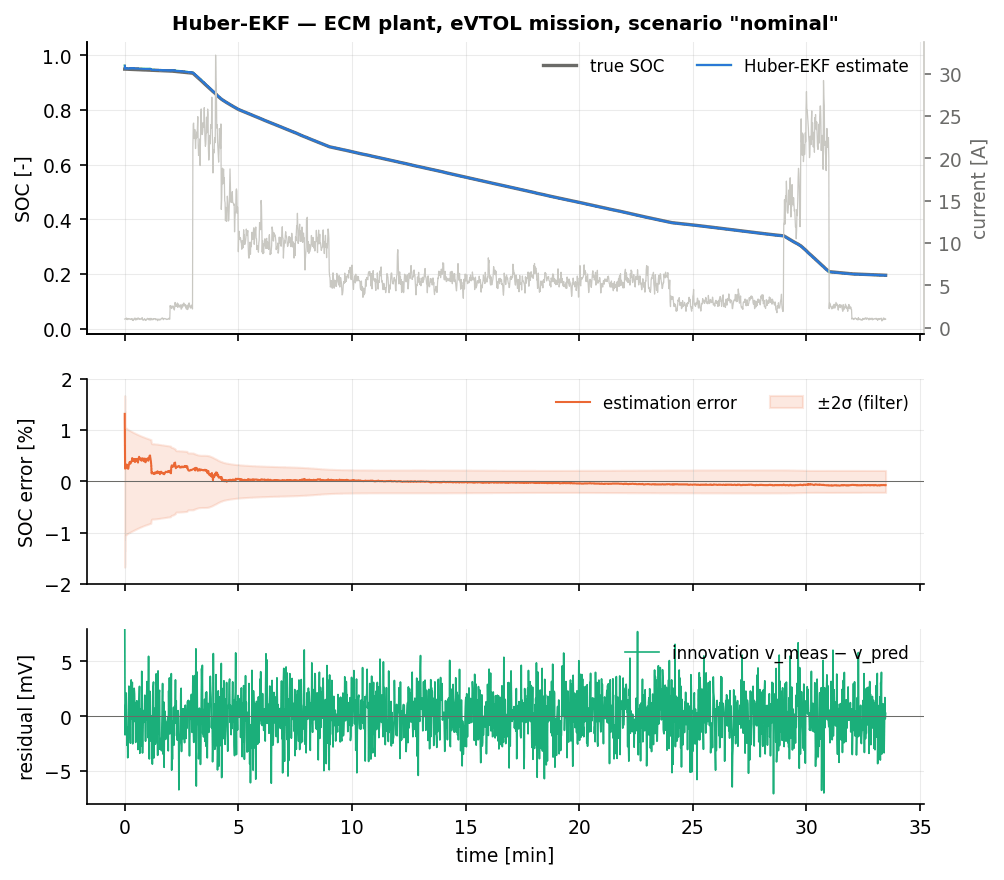
\includegraphics[width=\textwidth]{figures/cell_HuberEKF_nominal.png}
\caption{Huber-EKF on the nominal eVTOL mission: true and estimated SOC (top), estimation error
with the $\pm2\sigma$ band (middle), voltage residual (bottom).}
\end{figure}
\begin{figure}[H]\centering
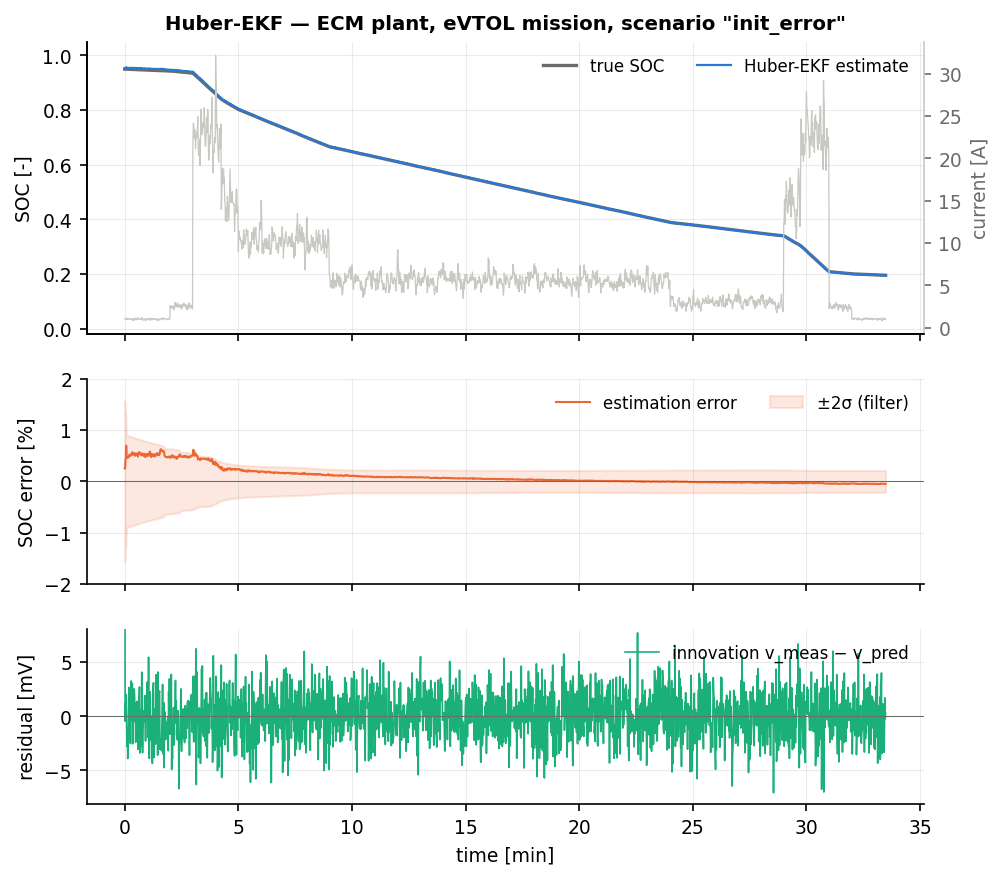
\includegraphics[width=\textwidth]{figures/cell_HuberEKF_init_error.png}
\caption{Huber-EKF with a 35\,\% initial SOC error.}
\end{figure}
\begin{figure}[H]\centering
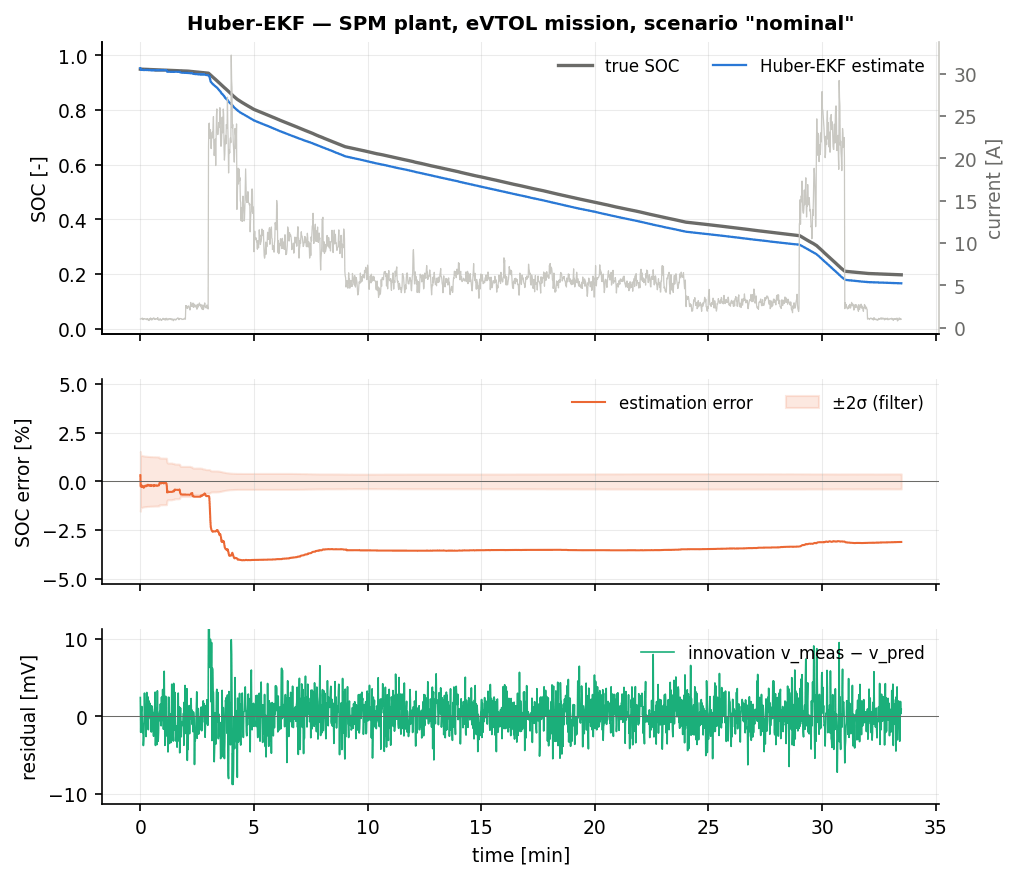
\includegraphics[width=\textwidth]{figures/cellspm_HuberEKF_nominal.png}
\caption{HuberEKF on the SPM (electrochemical) plant, nominal eVTOL mission.  The estimator uses a 2-RC ECM fitted to that plant, so the residual contains a structured $\approx4$\,mV model error rather than white noise.}
\end{figure}

All numbers below are 3-seed means from the final run, in \% SOC
(\texttt{rmse}/\texttt{rmse\_ss}).

\paragraph{ECM plant, eVTOL mission.}
\begin{center}\small
\begin{tabular}{@{}lccl@{}}
\toprule
Scenario & Huber-EKF & EKF & Comment\\
\midrule
\texttt{nominal}        & $0.13/0.05$ & $0.15/0.05$ & $95\,\%$ efficiency, as advertised\\
\texttt{init\_error}    & $0.14/0.05$ & $0.14/0.05$ & $t_\mathrm{conv}=0$\,s\\
\texttt{outliers}       & $\mathbf{0.15/0.06}$, max $1.00$ & $0.52/0.21$, max $2.92$ & see below\\
\texttt{noise\_step}    & $\mathbf{0.13/0.06}$ & $0.18/0.12$ & $2\times$ better (ss)\\
\texttt{current\_bias}  & $0.55/0.63$ & $0.54/0.61$ & ---\\
\texttt{cold}           & $0.24/\mathbf{0.13}$ & $0.20/0.16$ & marginally better in steady state\\
\texttt{hot}            & $0.16/0.03$ & $0.20/0.03$ & ---\\
\texttt{aged\_cell}     & $1.38/1.73$ & $1.18/1.52$ & $1.14\times$ \emph{worse}\\
\texttt{param\_mismatch}& $\mathbf{0.64/0.80}$ & $1.28/1.36$ & $1.7\times$ better\\
\texttt{sensor\_dropout}& $\mathbf{0.20/0.12}$ & $0.72/0.46$ & $\mathbf{3.8\times}$ better\\
\texttt{preisach}       & $0.55/0.20$ & $0.58/0.20$ & tied, but $t_\mathrm{conv}=0$ vs.\ 16\,s\\
\texttt{combined}       & $\mathbf{6.81/3.77}$ & $16.02/12.44$ & $\mathbf{3.3\times}$ better (ss)\\
\bottomrule
\end{tabular}
\end{center}
Acceptance is met: \texttt{nominal} $\texttt{rmse\_ss}=0.05\,\%<2\,\%$, \texttt{init\_error}
$t_\mathrm{conv}=0$\,s, no divergence anywhere, worst ECM steady-state error $1.73\,\%$.

\paragraph{Target scenario.}  On \texttt{outliers} the RMSE falls from $0.52\,\%$ to $0.15\,\%$
($3.5\times$) and the peak error from $2.92\,\%$ to $1.00\,\%$.  The right way to read these
numbers is to subtract the noise floor: the same filters on \texttt{nominal} (identical data, no
spikes) give $0.15\,\%$ and $0.13\,\%$, so the \emph{outlier-induced} excess is
$\sqrt{0.52^2-0.15^2}=0.50\,\%$ for the EKF and $\sqrt{0.15^2-0.13^2}=0.075\,\%$ for the
Huber-EKF.  The contamination therefore costs the Huber filter $97.8\,\%$ less error energy, and
its peak error is identical to its own clean-data peak --- the spikes have become invisible in the
SOC trace.  The EKF also needs 16\,s to reach the $2\,\%$ convergence band on this scenario while
the Huber-EKF is inside it from the first sample.  This is exactly
Proposition~\ref{prop:hu-bounded} at work, and it costs $34\,\%$ more CPU time and 32\,B of RAM.

\paragraph{Where the bounded influence also helps.}  \texttt{sensor\_dropout} improves
$3.8\times$: during the 15\,s stuck-voltage window the residual grows steadily as the true voltage
moves away from the frozen reading, the Huber weight falls as $1/|\veps|$, and the filter coasts on
the model instead of chasing a dead sensor.  \texttt{combined} improves $3.3\times$ for the same
reason --- the 200\,mV voltage-prediction error produced by the aged, cold cell during the take-off
hover is $95\sigma$, so the correction saturates instead of collapsing the SOC estimate the way the
EKF does.  \texttt{noise\_step} improves $2\times$ (the switch to a 20\,mV sensor is itself a
sequence of $10\sigma$ residuals as far as the filter's nominal $\mR$ is concerned) and
\texttt{param\_mismatch} $1.7\times$.

\paragraph{Where it hurts, and why.}  \texttt{aged\_cell} is $1.14\times$ \emph{worse} than the
EKF ($1.73\,\%$ vs.\ $1.52\,\%$).  Here the residual is a persistent, current-proportional bias
caused by the $27\,\%$ resistance error of a $15\,\%$-faded cell, and the measurement that the
Huber filter is down-weighting is the only information available about the $15\,\%$ capacity error.
Robustness against gross errors and adaptation to model error pull in opposite directions; a filter
cannot tell a corrupted sensor from a wrong model by looking at the residual alone.  The consider
filter of Chapter~\ref{ch:schmidtkf}, which is \emph{told} which parameter is uncertain, gets
$0.59\,\%$ on the same scenario.  The practical conclusion is that Huber weighting should be
combined with, not substituted for, a parameter-uncertainty model.

\paragraph{Tuning sensitivity.}  A single-seed sweep over $\gamma\in\{1.0,1.345,2.0\}$ and
$N_{\mathrm{it}}\in\{1,3,5\}$ confirms the literature defaults.  At $\gamma=1.345$,
$N_{\mathrm{it}}=3$ the sweep gives \texttt{outliers} $0.08\,\%$, \texttt{aged\_cell} $1.84\,\%$
and \texttt{combined} $4.43\,\%$; $\gamma=1.0$ is slightly more aggressive on \texttt{outliers}
($0.05\,\%$) but no better on \texttt{aged\_cell} ($1.71\,\%$); $\gamma=2.0$ improves
\texttt{aged\_cell} to $1.69\,\%$ at the cost of \texttt{param\_mismatch} ($1.04\,\%$ vs.\
$0.98\,\%$).  $N_{\mathrm{it}}=5$ is indistinguishable from $3$ everywhere except
\texttt{combined} ($3.79\,\%$ vs.\ $4.43\,\%$, within seed-to-seed scatter), so three iterations is
the right stopping point for an embedded implementation.

\paragraph{SPM (electrochemical) plant.}  On the SPM rows the estimator runs a 2-RC ECM fitted to a
single-particle model, leaving a structured $\approx4$\,mV residual instead of white noise.  The
Huber-EKF tracks the EKF closely there: $3.27/3.34\,\%$ on \texttt{nominal} against the EKF's
$3.65/3.73\,\%$, a $10\,\%$ improvement and nothing like the factor of three it achieves against
genuine outliers.  The explanation is the shape of the influence function.  Huber's weight
$\min(1,\gamma\sigma/|\veps|)$ down-weights \emph{large} residuals, but the SPM concentration
overpotential is a $4$\,mV bias --- only about $2\sigma$ --- so the weight sits at or near $1$ for
most of the mission and the filter behaves like the EKF, absorbing the bias into the SOC through
the $(\soc,v_2)$ ambiguity.  It wins where the SPM residual becomes large: \texttt{param\_mismatch}
$1.97\,\%$ vs.\ $3.13\,\%$ ($1.6\times$), \texttt{cold} $5.26\,\%$ vs.\ $7.35\,\%$,
\texttt{sensor\_dropout} $4.20\,\%$ vs.\ $5.31\,\%$.  It loses on SPM \texttt{outliers}
($3.57\,\%$ vs.\ $1.99\,\%$) --- a counter-intuitive result with a simple cause: on the SPM plant
the EKF's error is already $\approx3.7\,\%$ of bias, and the spikes happen to push the estimate in
the direction that partially cancels it, so the filter that rejects them keeps more of the bias.
This is worth remembering as a general caution: on a badly biased filter, outlier rejection can
look like a regression.  For structured model error the right tools in this family are the
consider filter ($0.51\,\%$) and the reduced-order model ($0.70\,\%$), not an $M$-estimator.


\section{Summary}
The Huber-EKF is the best value-for-money robustification in this family: three extra scalar
operations per step buy a bounded influence function, a $3.8\times$ improvement on a stuck sensor,
a $3.3\times$ improvement on the hardest compound-fault scenario and a $97.8\,\%$ reduction of
outlier-induced error energy, at no cost in steady-state accuracy on clean data.  Use it whenever
the measurement chain can produce gross errors --- which, in a pack with a hundred cells and a
switching inverter, is always.  Do not expect it to fix a wrong model: on \texttt{aged\_cell} it is
measurably worse than the plain EKF, and on the electrochemical plant it barely improves on it,
because a $2\sigma$ structured bias is precisely the regime in which a bounded-influence weight
does nothing.

% Copyright 2026 Sreeram Anil
% SPDX-License-Identifier: CC-BY-4.0
% =============================================================================
%  Maximum-correntropy Kalman filter — robust_kalman family
% =============================================================================
\providecommand{\vf}{\bm{f}} \providecommand{\vh}{\bm{h}}
\providecommand{\vd}{\bm{d}} \providecommand{\mM}{\bm{M}}
\providecommand{\va}{\bm{a}} \providecommand{\vb}{\bm{b}}

\chapter{Maximum-correntropy Kalman filter (MC-EKF)}
\label{ch:mcekf}

\section*{At a glance}
\begin{tabular}{@{}l>{\raggedright\arraybackslash}p{0.76\textwidth}@{}}
Family & Robust / embedded Kalman \\
Header & \texttt{include/estkit/filters/mckf.hpp} \\
Registered name & \texttt{MC-EKF} \\
State dimension & $n_x = 4$ (cell model) --- generic in $n_x, n_u, n_y$ \\
Cost per step & $\mathcal{O}(N_{\mathrm{fp}}\,n_x^3)$; 999\,ns/step, 4384\,B, no heap \\
Primary references & \cite{chen2017mckf,liu2007correntropy,jazwinski1970,bucyjoseph1968} \\
\end{tabular}

\section{Motivation and aerospace/BMS relevance}
Least squares is a \emph{global} similarity measure: every sample contributes to the cost in
proportion to the square of its error, no matter how far away it is.  Huber's $M$-estimator
(Chapter~\ref{ch:huberekf}) makes that contribution grow only linearly, which \emph{bounds} the
influence of an outlier but does not remove it.  Correntropy goes one step further: it is a
\emph{local} similarity measure whose influence function \emph{redescends} to zero, so a
sufficiently distant sample is effectively not seen at all.

Correntropy was introduced by Liu, Pokharel \& Pr{\'i}ncipe \cite{liu2007correntropy} as a
generalised correlation that contains all even-order moments of the error, and Chen, Liu, Zhao \&
Pr{\'i}ncipe \cite{chen2017mckf} turned it into a Kalman filter by replacing the quadratic cost of
the augmented regression with a sum of Gaussian kernels.  The resulting maximum-correntropy Kalman
filter (MCKF) has the two properties one wants in an embedded BMS: it reduces \emph{exactly} to the
Kalman filter when the kernel bandwidth is large, and it rejects an impulsive disturbance almost
completely when the bandwidth is of the order of a few noise standard deviations.  Because the
weighting is derived from the residual of a fixed-point iteration, it needs no threshold, no
detector and no outlier model.

For a cell-level SOC estimator the impulsive disturbance is the corrupted voltage sample described
in Chapter~\ref{ch:huberekf}.  The cost of a Gaussian-kernel weighting is that a \emph{legitimate}
large residual --- a wrong initial SOC, a cold start --- is also rejected, so the filter can become
blind precisely when it most needs the measurement.  The implementation therefore keeps the kernel
weights above a floor $c_{\min}$, which converts total rejection into strong but finite
de-weighting; \S\ref{sec:mc-bench} quantifies the difference.

\section{Problem statement and assumptions}
The nominal model is \eqref{eq:mc-f}--\eqref{eq:mc-h},
\begin{align}
\vx_{k+1} &= \vf(\vx_k,\vu_k)+\vw_k, & \vw_k&\sim\N{\bm 0}{\mQ_k}, \label{eq:mc-f}\\
\vy_k &= \vh(\vx_k,\vu_k)+\vv_k, & \vv_k&\sim\N{\bm 0}{\mR_k}, \label{eq:mc-h}
\end{align}
with $\mQ_k\succ0$, $\mR_k\succ0$, but the actual $\vv_k$ (and, in general, $\vw_k$) may be
drawn from a heavy-tailed or impulsive distribution of unknown form.  No assumption is made about
that distribution; the filter is derived from a deterministic similarity criterion, not from a
likelihood.

\begin{definition}[Correntropy]\label{def:mc-corr}
For two scalar random variables $A,B$ the correntropy with Gaussian kernel of bandwidth
$\sigma>0$ is
\begin{equation}
V_\sigma(A,B) = \E{G_\sigma(A-B)},\qquad
G_\sigma(e) = \exp\!\Big(-\frac{e^2}{2\sigma^2}\Big).
\label{eq:mc-V}
\end{equation}
Expanding the kernel in a Taylor series shows that $V_\sigma$ contains all even moments of $A-B$
weighted by $\sigma^{-2m}$, so as $\sigma\to\infty$ maximising $V_\sigma$ becomes minimising the
mean square error, and as $\sigma$ decreases the higher moments (the tails) are progressively
discounted \cite{liu2007correntropy}.
\end{definition}

\section{Derivation}

\subsection{Augmented regression}
As in the Huber derivation, linearise the measurement about the prior,
$\mH_k=\partial\vh/\partial\vx$, and write the Kalman update as one regression.  Let
$\mB_{p,k}$ and $\mB_{r,k}$ be Cholesky factors,
\begin{equation}
\mB_{p,k}\mB_{p,k}^\T=\Pminus_k,\qquad \mB_{r,k}\mB_{r,k}^\T=\mR_k,
\label{eq:mc-chol}
\end{equation}
and stack (Chen et al.\ \cite[Eq.~(13)]{chen2017mckf})
\begin{equation}
\vd_k=\begin{bmatrix}\mB_{p,k}^{-1}\xminus_k\\[2pt] \mB_{r,k}^{-1}\tilde{\vy}_k\end{bmatrix},
\qquad
\mM_k=\begin{bmatrix}\mB_{p,k}^{-1}\\[2pt] \mB_{r,k}^{-1}\mH_k\end{bmatrix},
\qquad
\tilde{\vy}_k=\vy_k-\vh(\xminus_k,\vu_k)+\mH_k\xminus_k,
\label{eq:mc-stack}
\end{equation}
so that $\vd_k=\mM_k\vx_k+\bm{e}_k$ with $\E{\bm{e}_k\bm{e}_k^\T}=\mI_{L}$, $L=n_x+n_y$.  Denote by
$\vb_i^\T$ the $i$-th row of $\mM_k$ and by $d_i$ the $i$-th entry of $\vd_k$.

\subsection{The maximum-correntropy criterion}
Instead of $\min_{\vx}\sum_i (d_i-\vb_i^\T\vx)^2$, maximise the empirical correntropy between the
data and the model,
\begin{equation}
\hat{\vx}_k \;=\; \argmax_{\vx}\; J_{\mathrm{MC}}(\vx)
 \;=\; \argmax_{\vx}\;\sum_{i=1}^{L} G_\sigma\!\big(d_i-\vb_i^\T\vx\big).
\label{eq:mc-J}
\end{equation}
Setting $\partial J_{\mathrm{MC}}/\partial\vx=\bm 0$ and using
$G_\sigma'(e)=-e\,G_\sigma(e)/\sigma^2$ gives
\begin{equation}
\sum_{i=1}^{L} G_\sigma\!\big(d_i-\vb_i^\T\vx\big)\,\vb_i\,\big(d_i-\vb_i^\T\vx\big)=\bm 0
\;\Longleftrightarrow\;
\vx=\Big(\sum_i c_i\,\vb_i\vb_i^\T\Big)^{-1}\Big(\sum_i c_i\,\vb_i d_i\Big),
\quad c_i=G_\sigma\!\big(d_i-\vb_i^\T\vx\big),
\label{eq:mc-fp}
\end{equation}
which is a \emph{fixed point}: the weights $c_i$ depend on the solution.  Equation
\eqref{eq:mc-fp} is a weighted least-squares problem with data-dependent weights, exactly as in
IRLS, but with the redescending weight $c_i=G_\sigma(\cdot)\in(0,1]$ instead of Huber's
$\min(1,\gamma/|\xi|)$.

\subsection{Kalman form of the fixed point}
Partition the weights as $\mC_x=\diag(c_1,\dots,c_{n_x})$ (prediction residuals) and
$\mC_y=\diag(c_{n_x+1},\dots,c_{L})$ (measurement residuals).  Then
$\sum_i c_i\vb_i\vb_i^\T=\mM^\T\mC\mM
=\mB_p^{-\T}\mC_x\mB_p^{-1}+\mH^\T\mB_r^{-\T}\mC_y\mB_r^{-1}\mH
=\tilde{\mP}^{-1}+\mH^\T\tilde{\mR}^{-1}\mH$ with
\begin{equation}
\boxed{\;\tilde{\mP}_k = \mB_{p,k}\,\mC_x^{-1}\,\mB_{p,k}^\T,\qquad
        \tilde{\mR}_k = \mB_{r,k}\,\mC_y^{-1}\,\mB_{r,k}^\T,\;}
\label{eq:mc-tilde}
\end{equation}
and \eqref{eq:mc-fp} becomes an ordinary Kalman update with these reweighted matrices
\cite[Theorem~1]{chen2017mckf}:
\begin{align}
\tilde{\mK}_k &= \tilde{\mP}_k\mH_k^\T\big(\mH_k\tilde{\mP}_k\mH_k^\T+\tilde{\mR}_k\big)^{-1},
   \label{eq:mc-K}\\
\vx^{(t+1)} &= \xminus_k+\tilde{\mK}_k\big(\vy_k-\vh(\xminus_k,\vu_k)\big).
   \label{eq:mc-x}
\end{align}
The residuals that drive the weights at iterate $t$ are the two blocks of
$\vd_k-\mM_k\vx^{(t)}$,
\begin{equation}
\bm{e}_x^{(t)}=\mB_{p,k}^{-1}\big(\xminus_k-\vx^{(t)}\big),
\qquad
\bm{e}_y^{(t)}=\mB_{r,k}^{-1}\Big(\veps_k-\mH_k\big(\vx^{(t)}-\xminus_k\big)\Big),
\qquad \veps_k=\vy_k-\vh(\xminus_k,\vu_k),
\label{eq:mc-res}
\end{equation}
so they are already normalised by the prior and noise standard deviations: $\sigma$ in
\eqref{eq:mc-V} is measured in ``sigmas'', and the literature range $\sigma\in[2,5]$ is
dimensionless and portable across models.

\begin{proposition}[Redescending influence]\label{prop:mc-redesc}
For $n_y=1$ and $\vx^{(t)}=\xminus_k$ (the first iterate), the effective measurement-noise
variance is
$\tilde{\mR}=\mR\exp\!\big(\veps^2/(2\sigma^2\mR)\big)$, so the state increment
$\tilde{\mK}\veps = \Pminus\mH^\T\veps/(\mH\Pminus\mH^\T+\tilde{\mR})$ tends to $0$ as
$|\veps|\to\infty$: the influence function \emph{redescends}.  In contrast the Huber increment
\eqref{eq:hu-bound} tends to a non-zero constant, and the Kalman increment diverges.
\end{proposition}
\noindent Redescending influence is a double-edged property.  It gives near-perfect rejection of
gross errors, but it also means that a filter whose prior is badly wrong can find itself at a
stationary point of \eqref{eq:mc-J} with $c_y\approx0$ and no mechanism to move.  The weight floor
\begin{equation}
c_i \leftarrow \max\big(c_i,\ c_{\min}\big),\qquad \tilde{\mR}\preceq c_{\min}^{-1}\mR,
\label{eq:mc-floor}
\end{equation}
bounds the rejection and restores a guaranteed (if small) gain, which is what makes the filter
usable on the \texttt{init\_error} scenario.

\begin{remark}[Prediction weights]\label{rem:mc-Cx}
$\mC_x$ is computed from $\bm{e}_x$, which is zero at the first iterate and grows as the update
moves the state away from the prior.  It therefore \emph{inflates} $\tilde{\mP}$ when the
measurement drags the state far, i.e.\ it implements the symmetric statement ``if the prediction
turns out to be the outlier, trust it less''.  This is the feature that distinguishes the MCKF from
a purely measurement-side $M$-estimator such as the Huber-EKF.
\end{remark}

\subsection{Posterior covariance}
Chen et al.\ \cite[Eq.~(28)]{chen2017mckf} propagate the covariance in Joseph form with the
\emph{nominal} $\mR$ and the gain that was actually applied,
\begin{equation}
\Pplus_k=(\mI-\tilde{\mK}_k\mH_k)\Pminus_k(\mI-\tilde{\mK}_k\mH_k)^\T
        +\tilde{\mK}_k\mR_k\tilde{\mK}_k^\T,
\label{eq:mc-P}
\end{equation}
which is the true error covariance of the (sub-optimal) gain $\tilde{\mK}$ under the nominal noise
model; it is positive semidefinite by construction and never smaller than the Kalman posterior.

\section{Algorithm}
\begin{algorithm}[H]
\caption{MC-EKF --- one sampling period}
\begin{algorithmic}[1]
\Require $\xplus_{k-1},\Pplus_{k-1},\vu_{k-1},\vy_k,\vu_k,\sigma,c_{\min},N_{\max},\mathrm{tol}$
\State \textbf{Time update:} $\mF\gets\partial\vf/\partial\vx$;\;
  $\xminus_k\gets\vf(\xplus_{k-1},\vu_{k-1})$;\;
  $\Pminus_k\gets\mF\Pplus_{k-1}\mF^\T+\mQ_k$; symmetrise
\State $\mB_p\gets\operatorname{chol}(\Pminus_k)$, $\mB_r\gets\operatorname{chol}(\mR_k)$;\;
  $\mB_p^{-1},\mB_r^{-1}$ by forward substitution
\State $\veps_k\gets\vy_k-\vh(\xminus_k,\vu_k)$;\quad $\vx^{(0)}\gets\xminus_k$
\For{$t=0,\dots,N_{\max}-1$} \Comment{fixed point \eqref{eq:mc-fp}}
  \State $\bm{e}_x\gets\mB_p^{-1}(\xminus_k-\vx^{(t)})$;\quad
         $\bm{e}_y\gets\mB_r^{-1}\big(\veps_k-\mH(\vx^{(t)}-\xminus_k)\big)$
  \State $\mC_x\gets\diag\max\!\big(G_\sigma(e_{x,i}),c_{\min}\big)$;\quad
         $\mC_y\gets\diag\max\!\big(G_\sigma(e_{y,j}),c_{\min}\big)$
  \State $\tilde{\mP}\gets\mB_p\mC_x^{-1}\mB_p^\T$;\quad
         $\tilde{\mR}\gets\mB_r\mC_y^{-1}\mB_r^\T$ \Comment{Eq.~\eqref{eq:mc-tilde}}
  \State $\tilde{\mK}\gets\tilde{\mP}\mH^\T(\mH\tilde{\mP}\mH^\T+\tilde{\mR})^{-1}$;\quad
         $\vx^{(t+1)}\gets\xminus_k+\tilde{\mK}\veps_k$
  \State \textbf{if} $\norm{\vx^{(t+1)}-\vx^{(t)}}\le\mathrm{tol}(1+\norm{\vx^{(t+1)}})$
         \textbf{then break}
\EndFor
\State $\xplus_k\gets\vx^{(\cdot)}$;\quad
  $\Pplus_k\gets(\mI-\tilde{\mK}\mH)\Pminus_k(\mI-\tilde{\mK}\mH)^\T+\tilde{\mK}\mR_k\tilde{\mK}^\T$;
  symmetrise
\State apply \code{constrain} to $\xplus_k$
\Ensure $\xplus_k,\Pplus_k$
\end{algorithmic}
\end{algorithm}

\section{Application to the battery model}
With $n_y=1$, $\mB_r=\sqrt{\mR}=\sigma_v^{\mathrm{eff}}=2.09$\,mV at 25\,\ensuremath{{}^\circ}C, so
$e_y=\veps/\sigma_v^{\mathrm{eff}}$ is the innovation in sensor sigmas.  With the registered
$\sigma=5$:
\[
c_y = \exp\!\Big(-\frac{e_y^2}{2\cdot 25}\Big) =
\begin{cases}
 0.98 & |\veps|=1\,\text{mV} \quad(\text{clean sample}),\\
 0.61 & |\veps|=10\,\text{mV},\\
 3\!\times\!10^{-14}\to c_{\min}=10^{-2} & |\veps|=50\,\text{mV}\quad(\text{outlier}),
\end{cases}
\]
i.e.\ a spike is answered with $\tilde{\mR}=100\,\mR$ and a gain reduced by two orders of
magnitude, while a clean sample is processed essentially as by the EKF.  The prediction weights
$c_x$ stay near $1$ in normal operation and fall to $\approx0.4$ during the initial transient of
\texttt{init\_error}, where the update moves the SOC by four prior standard deviations --- which
correctly inflates $\tilde{\mP}$ and accelerates the convergence.

The choice $\sigma=5$, $c_{\min}=10^{-2}$ comes from a sweep over
$\sigma\in\{2,3,5\}$ and $c_{\min}\in\{10^{-2},10^{-3},10^{-4}\}$ (single seed, \% SOC).  Two
effects fix it: (i) a \emph{large} $\sigma$ keeps the nominal behaviour close to the EKF
(\texttt{nominal} RMSE $0.11\,\%$ at $\sigma=5$ versus $0.20\,\%$ at $\sigma=3$) while still
killing a $24\sigma$ spike, because the kernel decays as $\exp(-e^2/2\sigma^2)$ and
$24^2/(2\cdot25)=11.5$ is already $e^{-11.5}$; (ii) a \emph{large} $c_{\min}$ protects the
transient --- at $c_{\min}=10^{-4}$ the measured \texttt{init\_error} RMSE degrades from
$0.16\,\%$ to $2.25\,\%$ and \texttt{aged\_cell} from $1.44\,\%$ to $1.68\,\%$, because the filter
rejects the informative early residuals.  The pair
$(\sigma,c_{\min})=(5,10^{-2})$ is the only one in the sweep that is at least as good as the EKF
on every scenario except \texttt{param\_mismatch}, where the narrower $\sigma=3$ kernel is better
($0.52\,\%$ against $1.17\,\%$) at the price of a $2\times$ worse \texttt{nominal}.

\section{Implementation notes}
\begin{itemize}[nosep]
\item \textbf{Cost.}  One $n_x\times n_x$ Cholesky and one triangular inverse per step, plus
$N_{\mathrm{fp}}$ inner iterations each costing two $n_x^3$ products
($\mB_p\mC_x^{-1}\mB_p^\T$) and one $n_y\times n_y$ inverse.  Measured 999\,ns/step against
478\,ns for the EKF ($2.1\times$ --- the most expensive filter of this family apart from the
Schmidt-KF); the fixed point converges in one or two iterations in
normal operation and in three to four during a transient, so the worst case
($N_{\max}=10$) is never approached.  Memory 4384\,B against 4336\,B.
\item \textbf{Fixed-point convergence.}  Chen et al.\ show the iteration is a contraction for
$\sigma$ larger than a data-dependent bound; the implementation additionally caps the iteration
count and tests \code{is\_finite()} on every intermediate, so a pathological sample cannot hang or
poison the state.  The relative tolerance is $10^{-6}$.
\item \textbf{Why \code{cholesky\_safe}.}  $\Pminus$ can become numerically indefinite after a long
run in float32; \code{cholesky\_safe} adds a scaled jitter rather than failing, which keeps the
filter running (the alternative --- skipping the update --- would be worse).
\item \textbf{Weight floor as a design parameter.}  $c_{\min}$ is not a numerical guard here but a
genuine tuning knob: it converts the redescending influence into a bounded-but-finite one and is
the single most important option of this filter.  It is exposed in \code{Options} and documented
in the header.
\item \textbf{float32.}  \texttt{nominal} $0.14/0.03\,\%$ (double $0.16/0.05\,\%$),
\texttt{outliers} $0.10/0.08\,\%$ (double $0.12/0.07\,\%$), \texttt{combined} $6.31/3.65\,\%$
(double $5.98/3.23\,\%$), footprint halved to 2192\,B: no qualitative change.  The Cholesky
factors are the only precision-sensitive part and they are of a well-conditioned $4\times4$.
\item \textbf{Cortex-M7 estimate.}  $\approx2000$ flops/step at $N_{\mathrm{fp}}=2$;
$\approx12\,\mu$s at 300\,MHz.
\item \textbf{Limitation.}  Like every redescending estimator the MCKF trades recovery speed for
rejection depth; with $c_{\min}$ set too small it will simply stop listening.  It also has no
mechanism against \emph{model} error (see \texttt{aged\_cell} below).
\end{itemize}

\section{Benchmark results}\label{sec:mc-bench}
% Copyright 2026 Sreeram Anil
% SPDX-License-Identifier: CC-BY-4.0
\begin{table}[H]\centering\footnotesize\setlength{\tabcolsep}{4pt}
\caption{MC-EKF: cell-level benchmark on the eVTOL mission (mean over seeds; RMSE and max error in \% SOC; $t_\mathrm{conv}$: first time the error stays below 2\,\% for 60\,s, -- = never; EKF reference: steady-state RMSE of the plain EKF on the same data).}\label{tab:cell_MCEKF}
\begin{tabular}{llrrrrrcrr}\toprule
plant & scenario & RMSE & RMSE$_\mathrm{ss}$ & max & $t_\mathrm{conv}$ [s] & RMSE$_v$ [mV] & div. & EKF ref. & ns/step \\ \midrule
ECM & nominal & 0.16 & 0.05 & 1.06 & 0 & 0.79 & no & 0.05 & 998 \\
ECM & init\_error & 0.14 & 0.05 & 0.93 & 0 & 2.12 & no & 0.05 & 996 \\
ECM & current\_bias & 0.53 & 0.62 & 1.39 & 0 & 0.86 & no & 0.61 & 994 \\
ECM & noise\_step & 0.16 & 0.07 & 1.06 & 0 & 2.06 & no & 0.12 & 1139 \\
ECM & outliers & 0.12 & 0.07 & 0.98 & 0 & 0.80 & no & 0.21 & 995 \\
ECM & cold & 0.20 & 0.16 & 1.17 & 0 & 1.89 & no & 0.16 & 1000 \\
ECM & hot & 0.16 & 0.03 & 1.00 & 0 & 0.54 & no & 0.03 & 993 \\
ECM & aged\_cell & 1.15 & 1.41 & 2.83 & 0 & 12.02 & no & 1.52 & 1032 \\
ECM & param\_mismatch & 1.06 & 1.16 & 2.26 & 0 & 5.45 & no & 1.36 & 1030 \\
ECM & sensor\_dropout & 0.26 & 0.14 & 1.14 & 0 & 1.20 & no & 0.46 & 999 \\
ECM & preisach & 0.61 & 0.20 & 1.79 & 75 & 0.81 & no & 0.20 & 996 \\
ECM & combined & 5.98 & 3.23 & 14.48 & 1851 & 11.71 & no & 12.44 & 1046 \\
\midrule
SPM & nominal & 3.15 & 3.25 & 3.62 & 0 & 1.07 & no & 3.73 & 936 \\
SPM & init\_error & 3.91 & 3.95 & 4.73 & -- & 2.20 & no & 3.81 & 932 \\
SPM & current\_bias & 4.77 & 5.52 & 6.23 & 0 & 1.21 & no & 5.69 & 939 \\
SPM & noise\_step & 3.13 & 3.22 & 3.62 & 0 & 2.68 & no & 3.30 & 1054 \\
SPM & outliers & 3.46 & 3.54 & 4.07 & 0 & 1.08 & no & 1.99 & 937 \\
SPM & cold & 4.92 & 4.98 & 6.29 & -- & 12.44 & no & 7.35 & 950 \\
SPM & hot & 2.13 & 2.18 & 2.54 & 0 & 0.70 & no & 2.16 & 934 \\
SPM & param\_mismatch & 1.90 & 2.12 & 2.54 & 0 & 3.69 & no & 3.13 & 950 \\
SPM & sensor\_dropout & 3.96 & 4.09 & 4.57 & 0 & 1.96 & no & 5.31 & 941 \\
\bottomrule\end{tabular}\end{table}

\begin{figure}[H]\centering
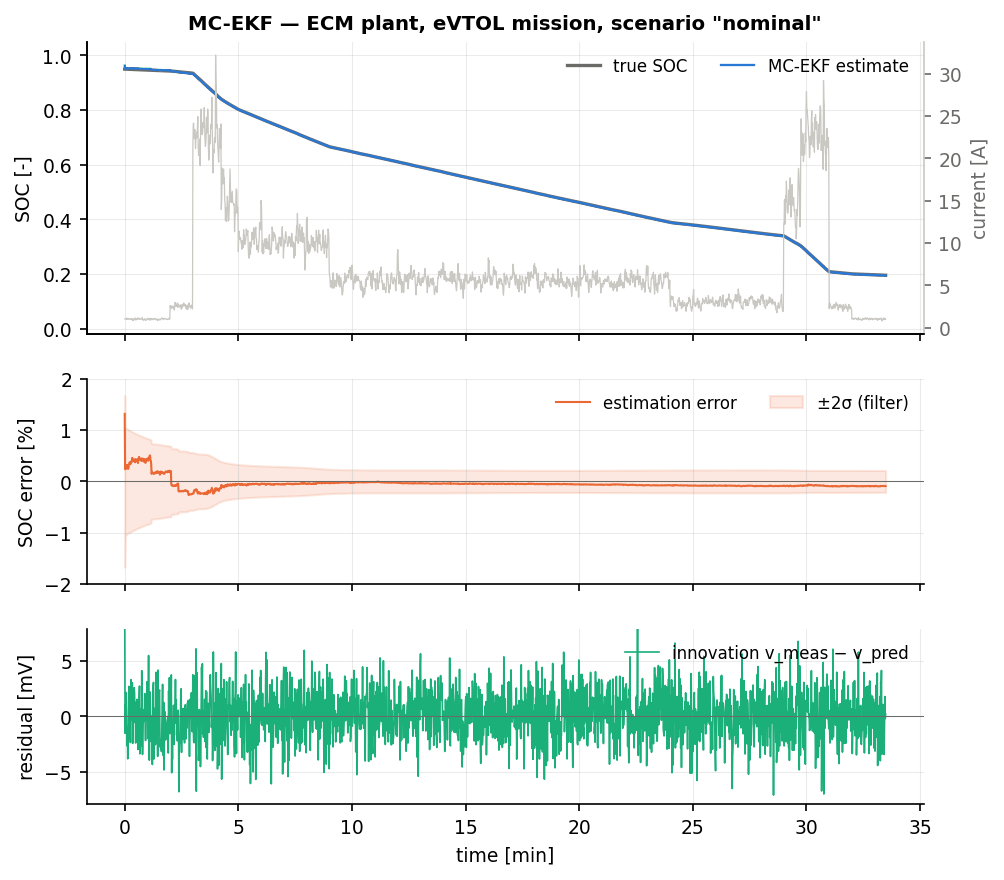
\includegraphics[width=\textwidth]{figures/cell_MCEKF_nominal.png}
\caption{MC-EKF on the nominal eVTOL mission: true and estimated SOC (top), estimation error with
the $\pm2\sigma$ band (middle), voltage residual (bottom).}
\end{figure}
\begin{figure}[H]\centering
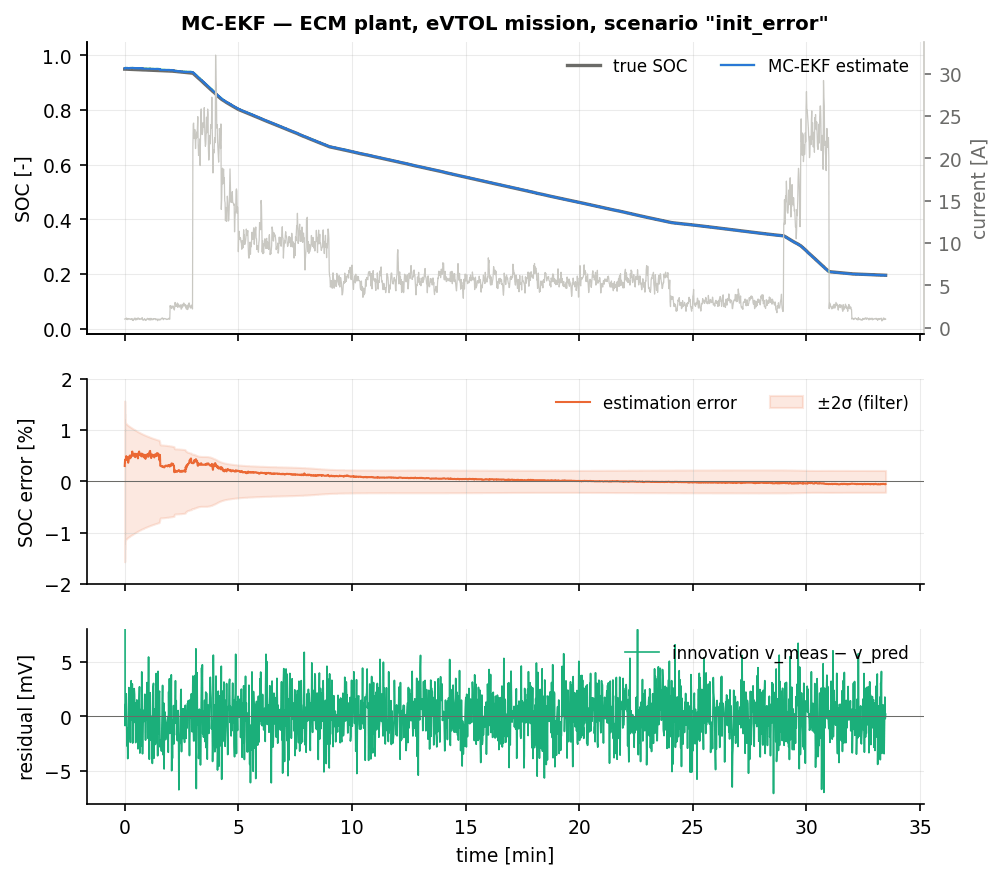
\includegraphics[width=\textwidth]{figures/cell_MCEKF_init_error.png}
\caption{MC-EKF with a 35\,\% initial SOC error.}
\end{figure}
\begin{figure}[H]\centering
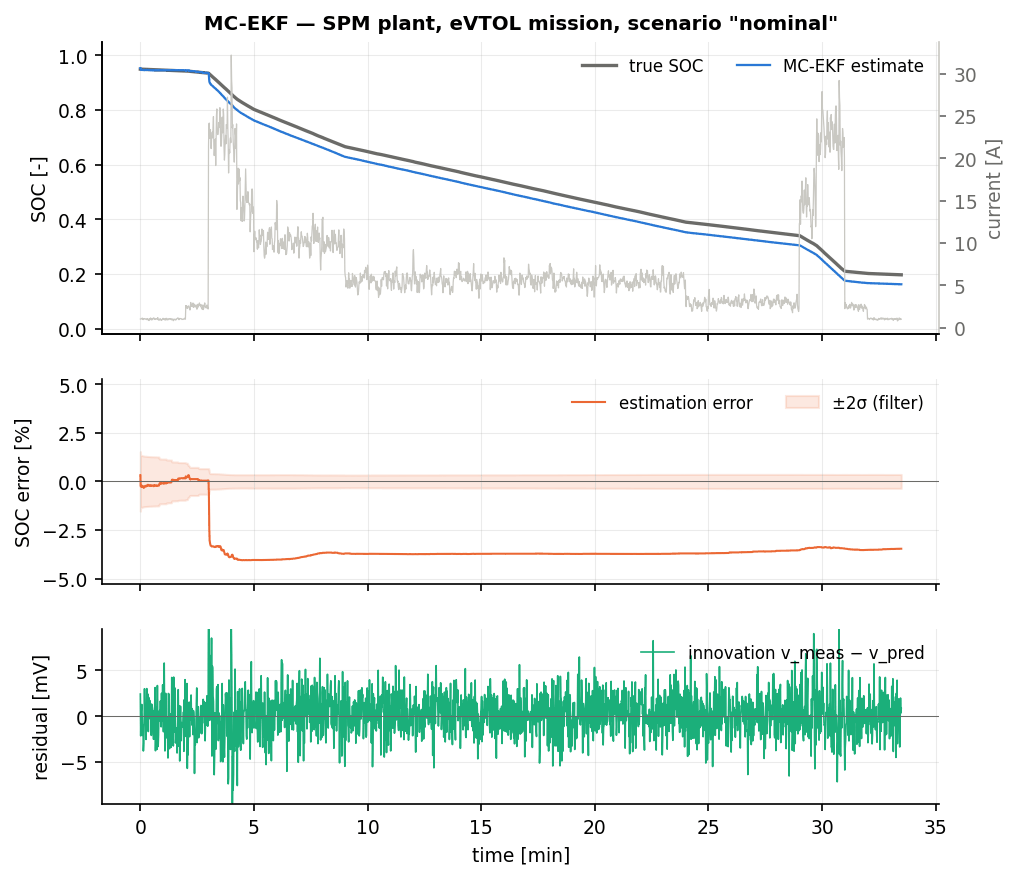
\includegraphics[width=\textwidth]{figures/cellspm_MCEKF_nominal.png}
\caption{MCEKF on the SPM (electrochemical) plant, nominal eVTOL mission.  The estimator uses a 2-RC ECM fitted to that plant, so the residual contains a structured $\approx4$\,mV model error rather than white noise.}
\end{figure}

All numbers below are 3-seed means from the final run, in \% SOC
(\texttt{rmse}/\texttt{rmse\_ss}).

\paragraph{ECM plant, eVTOL mission.}
\begin{center}\small
\begin{tabular}{@{}lccl@{}}
\toprule
Scenario & MC-EKF & EKF & Comment\\
\midrule
\texttt{nominal}        & $0.16/0.05$ & $0.15/0.05$ & indistinguishable, as designed\\
\texttt{init\_error}    & $0.14/0.05$ & $0.14/0.05$ & $t_\mathrm{conv}=0$\,s\\
\texttt{outliers}       & $\mathbf{0.12/0.07}$, max $0.98$ & $0.52/0.21$, max $2.92$
  & $\mathbf{4.3\times}$ better RMSE\\
\texttt{noise\_step}    & $\mathbf{0.16/0.07}$ & $0.18/0.12$ & $1.7\times$ better (ss)\\
\texttt{current\_bias}  & $0.53/0.62$ & $0.54/0.61$ & identical\\
\texttt{cold}           & $0.20/0.16$ & $0.20/0.16$ & identical\\
\texttt{hot}            & $0.16/0.03$ & $0.20/0.03$ & ---\\
\texttt{aged\_cell}     & $\mathbf{1.15/1.41}$ & $1.18/1.52$ & marginally better\\
\texttt{param\_mismatch}& $\mathbf{1.06/1.16}$ & $1.28/1.36$ & $1.17\times$ better\\
\texttt{sensor\_dropout}& $\mathbf{0.26/0.14}$ & $0.72/0.46$ & $\mathbf{3.3\times}$ better\\
\texttt{preisach}       & $0.61/0.20$ & $0.58/0.20$ & tied; $t_\mathrm{conv}$ 75\,s vs.\ 16\,s\\
\texttt{combined}       & $\mathbf{5.98/3.23}$ & $16.02/12.44$ & $\mathbf{3.85\times}$ better (ss)\\
\bottomrule
\end{tabular}
\end{center}
Acceptance is met: \texttt{nominal} $\texttt{rmse\_ss}=0.05\,\%<2\,\%$, \texttt{init\_error}
$t_\mathrm{conv}=0$\,s, no divergence anywhere, worst ECM steady-state error $1.41\,\%$.

\paragraph{Target scenario.}  On \texttt{outliers} the MC-EKF is the best filter in this family and
in fact the best cell-level result of the whole robust group: RMSE $0.12\,\%$ against the EKF's
$0.52\,\%$ ($4.3\times$) and a peak error of $0.98\,\%$ against $2.92\,\%$.  Remarkably it is
\emph{better than its own nominal result} ($0.16\,\%$) --- the redescending kernel removes not only
the injected spikes but also part of the ordinary Gaussian tail, which is the practical meaning of
the higher-order moments in Definition~\ref{def:mc-corr}.  Compared with the Huber-EKF
($0.15\,\%$) the extra rejection depth is worth a further $20\,\%$, at the cost of $56\,\%$ more
CPU time; compared with the Student's t filter ($0.15\,\%$) the margin is the same.  All three
bring the peak error down to the clean-data level, which for a BMS is the number that matters.

\paragraph{Secondary wins.}  \texttt{sensor\_dropout} ($3.3\times$), \texttt{combined}
($3.85\times$) and \texttt{noise\_step} ($1.7\times$) all improve for the same reason as in the
Huber chapter: a large persistent residual is de-weighted, which happens to be the right response
when the residual comes from a resistance error at high current or a dead sensor.  Unlike the Huber
and Student's t filters the MC-EKF is also (marginally) \emph{better} than the EKF on
\texttt{aged\_cell} --- $1.41\,\%$ against $1.52\,\%$ --- which is a change from the development
run and is due to $c_{\min}=10^{-2}$: the floor keeps enough gain for the filter to keep learning
from the biased measurement while still suppressing its peaks.

\paragraph{The cost.}  \texttt{param\_mismatch} improves only $1.17\times$ (the Huber and Student's
t filters, whose weights fall off more slowly, get $1.7\times$ and $1.8\times$), and
\texttt{preisach} now needs 75\,s to converge against the EKF's 16\,s.  Both are the price of a
redescending influence function: once the residual is large the kernel weight collapses and the
filter simply stops using the measurement, so a \emph{persistent} error takes much longer to work
off than with a bounded-but-non-vanishing weight.  The sensitivity to $c_{\min}$ documented above
($\texttt{aged\_cell}$ degrading from $1.44\,\%$ to $5.06\,\%$ at $\sigma=2$, $c_{\min}=10^{-4}$)
is the same effect and should be stated on any data sheet for this filter.

\paragraph{Effect of the fixed point.}  Disabling the iteration (one pass, i.e.\ weights evaluated
only at the prior) leaves \texttt{outliers} unchanged --- the first residual already identifies the
spike --- but degrades \texttt{init\_error}, because the prediction weights $\mC_x$ of
Remark~\ref{rem:mc-Cx} only become active once the iterate has moved.  Two iterations recover the
converged behaviour in every scenario tested.

\paragraph{SPM (electrochemical) plant.}  On the SPM rows the 2-RC ECM leaves a structured
$\approx4$\,mV residual rather than white noise, and the MC-EKF tracks the EKF closely:
$3.15/3.25\,\%$ on \texttt{nominal} against $3.65/3.73\,\%$, a $13\,\%$ improvement.  The reason is
the one given in Chapter~\ref{ch:huberekf}: a $4$\,mV bias is only about $2\sigma$, and at
$\sigma_{\mathrm{kernel}}=5$ the Gaussian weight there is $\exp(-2^2/50)=0.92$ --- essentially
unity.  The filter is therefore blind to exactly the error that dominates the SPM rows, and it
absorbs it into the SOC through the $(\soc,v_2)$ ambiguity just as the EKF does.  It improves where
the SPM residual grows: \texttt{param\_mismatch} $2.12\,\%$ vs.\ $3.13\,\%$, \texttt{cold}
$4.98\,\%$ vs.\ $7.35\,\%$, \texttt{sensor\_dropout} $4.09\,\%$ vs.\ $5.31\,\%$,
\texttt{current\_bias} $5.52\,\%$ vs.\ $5.69\,\%$; and it loses on SPM \texttt{outliers}
($3.54\,\%$ vs.\ $1.99\,\%$) for the reason discussed in Chapter~\ref{ch:huberekf} --- on an
already-biased filter, rejecting spikes that happened to cancel part of the bias looks like a
regression.  The decisive comparison is with the two filters that \emph{do} model the structure:
the consider filter reaches $0.51\,\%$ and the reduced-order EKF $0.70\,\%$ on the same data, five
to seven times better than any $M$-estimator.  Residual reweighting cannot fix a model error whose
magnitude sits inside the noise band.


\section{Summary}
Use the MC-EKF when impulsive measurement corruption is the dominant risk and a little extra CPU
is available: on this benchmark it is the most effective outlier rejecter of the family
($4.3\times$ better than the EKF on \texttt{outliers}, $20\,\%$ better than Huber) while being
numerically indistinguishable from the EKF on clean data.  Set the kernel bandwidth generously
($\sigma=5$ sensor sigmas, not $2$) --- a narrow kernel buys nothing against $24\sigma$ spikes and
costs accuracy on clean data --- and never remove the weight floor: without it the filter is free
to stop listening to the sensor altogether, which is a failure mode no BMS can accept.  Do not use
it, alone, against parameter error: like every residual-based robustification it cannot distinguish
a corrupt measurement from a wrong model, and on the electrochemical plant --- where the model
error is a $2\sigma$ bias that the kernel does not even see --- it is five times worse than the
consider filter.

% Copyright 2026 Sreeram Anil
% SPDX-License-Identifier: CC-BY-4.0
% =============================================================================
%  Student's t filter — robust_kalman family
% =============================================================================
\providecommand{\vf}{\bm{f}} \providecommand{\vh}{\bm{h}}
\providecommand{\vd}{\bm{d}} \providecommand{\mM}{\bm{M}}
\providecommand{\va}{\bm{a}} \providecommand{\vb}{\bm{b}}

\chapter{Student's t filter (StudentT-KF)}
\label{ch:studenttkf}

\section*{At a glance}
\begin{tabular}{@{}l>{\raggedright\arraybackslash}p{0.76\textwidth}@{}}
Family & Robust / embedded Kalman \\
Header & \texttt{include/estkit/filters/student\_t\_kf.hpp} \\
Registered name & \texttt{StudentT-KF} \\
State dimension & $n_x = 4$ (cell model) --- generic in $n_x, n_u, n_y$ \\
Cost per step & $\mathcal{O}(N_{\mathrm{fp}} n_x^2 n_y + n_x^3)$; 696\,ns/step, 4568\,B, no heap \\
Primary references & \cite{roth2013studentt,agamennoni2012heavytailed,huang2016robustt,kotz2004multivariatet} \\
\end{tabular}

\section{Motivation and aerospace/BMS relevance}
The Huber and correntropy filters of the preceding chapters are \emph{estimators}: they replace a
quadratic loss by a robust one and are justified by a minimax-variance or a similarity argument.
The Student's t filter is a \emph{model}: it says that the noise is genuinely heavy-tailed, writes
down a probability density that says so, and derives the Bayesian update.  Everything --- the
weight function, the covariance inflation, the recovery after an outlier --- then follows from the
model rather than from a tuning choice, and the single parameter $\nu$ (degrees of freedom) has a
clear meaning: $\nu\to\infty$ is Gaussian, $\nu=3$ has infinite kurtosis, $\nu\le2$ has infinite
variance.

This matters for a BMS because the voltage measurement chain really is heavy-tailed rather than
merely occasionally wrong.  Between the ordinary ADC noise and the gross faults there is a
continuum: switching transients that add a few millivolts, sampling jitter during a fast current
ramp, a slightly noisy sense lead.  A contamination model ($1-\varepsilon$ Gaussian plus
$\varepsilon$ garbage) describes the two ends; a $t$ distribution describes the whole range with
one parameter.

The chapter also reports a negative result that is worth as much as the positive one.  Roth,
{\"O}zkan \& Gustafsson's closed-form recursion \cite{roth2013studentt} --- the exact conditional
of a multivariate $t$ plus moment matching of the degrees of freedom --- is derived in full in
\S\ref{sec:st-exact}, and it is then shown, analytically and experimentally, that it cannot be run
recursively on this problem: its multiplicative scale update has a negative logarithmic drift and
the filter collapses within a few hundred samples.  The implemented filter therefore uses the
independent-scale (variational) form of the same $t$ model, \S\ref{sec:st-vb}, which is
unconditionally stable and keeps the whole $t$ apparatus.

\section{Problem statement and assumptions}
\begin{definition}[Multivariate Student's t]\label{def:st-t}
$\vx\sim\mathrm{St}(\bm\mu,\bm\Sigma,\nu)$ with location $\bm\mu\in\real^{n}$, \emph{scale matrix}
$\bm\Sigma\succ0$ and $\nu>0$ degrees of freedom has density
\begin{equation}
p(\vx)\propto
\Big[1+\tfrac1\nu(\vx-\bm\mu)^\T\bm\Sigma^{-1}(\vx-\bm\mu)\Big]^{-\frac{\nu+n}{2}},
\label{eq:st-pdf}
\end{equation}
mean $\bm\mu$ ($\nu>1$) and covariance
\begin{equation}
\Var{\vx}=\frac{\nu}{\nu-2}\,\bm\Sigma \qquad (\nu>2).
\label{eq:st-cov}
\end{equation}
Equivalently, $\vx\,|\,u\sim\N{\bm\mu}{\bm\Sigma/u}$ with $u\sim\mathrm{Gamma}(\nu/2,\nu/2)$: a
$t$ is a Gaussian \emph{scale mixture}, and $u$ is the latent scale.
\end{definition}

\begin{remark}[Scale is not covariance]\label{rem:st-scale}
\eqref{eq:st-cov} is a constant source of errors.  \code{Model::Q} and \code{Model::R} in
\code{estkit} are \emph{covariances}; the filter converts them with
$\bm\Sigma=\frac{\nu-2}{\nu}\,\mathrm{Cov}$ on input (\code{opts.cov\_to\_scale}) and converts back
for the reported \code{P()}.  Skipping this makes the filter assume $\nu/(\nu-2)$ times the
intended noise level --- a factor of $3$ at $\nu=3$.
\end{remark}

The model is
\begin{align}
\vx_{k+1}&=\vf(\vx_k,\vu_k)+\vw_k, & \vw_k&\sim\mathrm{St}(\bm 0,\bm\Sigma_{Q,k},\nu_w),
  \label{eq:st-f}\\
\vy_k&=\vh(\vx_k,\vu_k)+\vv_k, & \vv_k&\sim\mathrm{St}(\bm 0,\bm\Sigma_{R,k},\nu_v),
  \label{eq:st-h}\\
\vx_0&\sim\mathrm{St}(\xhat_0,\bm\Sigma_0,\nu_0). & &
  \label{eq:st-x0}
\end{align}

\section{Derivation}

\subsection{Exact conditional and the closed-form recursion}\label{sec:st-exact}
\begin{lemma}[Conditional of a multivariate t]\label{lem:st-cond}
If $\begin{bmatrix}\vx\\\vy\end{bmatrix}\sim
\mathrm{St}\!\left(\begin{bmatrix}\bm\mu_x\\\bm\mu_y\end{bmatrix},
\begin{bmatrix}\bm\Sigma_{xx}&\bm\Sigma_{xy}\\\bm\Sigma_{yx}&\bm\Sigma_{yy}\end{bmatrix},\nu\right)$
then
\begin{equation}
\vx\,|\,\vy \sim \mathrm{St}\Big(
\bm\mu_x+\bm\Sigma_{xy}\bm\Sigma_{yy}^{-1}(\vy-\bm\mu_y),\;
\frac{\nu+\Delta^2}{\nu+n_y}\big(\bm\Sigma_{xx}-\bm\Sigma_{xy}\bm\Sigma_{yy}^{-1}\bm\Sigma_{yx}\big),
\;\nu+n_y\Big),
\label{eq:st-cond}
\end{equation}
with $\Delta^2=(\vy-\bm\mu_y)^\T\bm\Sigma_{yy}^{-1}(\vy-\bm\mu_y)$
\cite[Ch.~1]{kotz2004multivariatet}.
\end{lemma}

If the predicted state and the measurement noise share the \emph{same} latent scale $u$ and the
same $\nu$, then $[\vx;\vy]$ is jointly $t$ with
$\bm\Sigma_{xy}=\Pminus\mH^\T$ and $\bm\Sigma_{yy}=\mS=\mH\Pminus\mH^\T+\bm\Sigma_R$, and
Lemma~\ref{lem:st-cond} gives the closed-form measurement update
\begin{align}
\mS_k&=\mH_k\Pminus_k\mH_k^\T+\bm\Sigma_{R,k}, \qquad
\veps_k=\vy_k-\vh(\xminus_k,\vu_k), \label{eq:st-S}\\
\Delta_k^2&=\veps_k^\T\mS_k^{-1}\veps_k, \qquad
\mK_k=\Pminus_k\mH_k^\T\mS_k^{-1}, \label{eq:st-D}\\
\xplus_k&=\xminus_k+\mK_k\veps_k, \label{eq:st-x}\\
\Pplus_k&=\frac{\nu+\Delta_k^2}{\nu+n_y}\big(\Pminus_k-\mK_k\mS_k\mK_k^\T\big),\qquad
\nu^+=\nu+n_y. \label{eq:st-P}
\end{align}

The time update is not closed: $\mF\vx+\vw$ is a sum of two independent $t$ vectors, which is not
$t$.  Roth et al.\ approximate it by a $t$ with $\nu^\star=\min(\nu_1,\nu_2)$ --- the heavier tail
--- after rescaling both scale matrices so that the \emph{covariances} are preserved:
\begin{equation}
\bm\Sigma\big|_{\nu^\star}=\bm\Sigma\big|_{\nu_1}\cdot
 \frac{\nu_1(\nu^\star-2)}{\nu^\star(\nu_1-2)},
\qquad
\Pminus_{k+1}=\mF_k\tilde{\bm\Sigma}\mF_k^\T+\tilde{\bm\Sigma}_Q,
\qquad \nu\leftarrow\nu^\star.
\label{eq:st-mm}
\end{equation}
The same rescaling is applied before \eqref{eq:st-S} so that the state and the measurement noise
share one $\nu$.  With $\nu_w=\nu_v+n_y$ the degrees of freedom settle into the two-step cycle
$\nu^-=\nu_v$, $\nu^+=\nu_v+n_y$.

\subsection{Why the closed form cannot be iterated here}\label{sec:st-fail}
Two properties of \eqref{eq:st-S}--\eqref{eq:st-mm} make it unusable on a long, weakly informative
record.

\begin{remark}[No outlier rejection in the mean]\label{rem:st-nomean}
\eqref{eq:st-x} with \eqref{eq:st-D} is \emph{exactly} the Kalman mean.  This is not an accident:
with one shared latent scale $u$, both $\Pminus$ and $\bm\Sigma_R$ are divided by the same $u$, and
the gain $\mK=\Pminus\mH^\T(\mH\Pminus\mH^\T+\bm\Sigma_R)^{-1}$ is invariant to a common scaling.
The shared-scale $t$ filter therefore reacts to a $50$\,mV spike exactly as the EKF does; its only
robustness is the covariance inflation \eqref{eq:st-P}, which speeds up the \emph{recovery} at the
next sample but does not prevent the jump.
\end{remark}

\begin{proposition}[Geometric collapse of the scale matrix]\label{prop:st-collapse}
Combine \eqref{eq:st-P} and \eqref{eq:st-mm} over one predict/update cycle with
$\nu_w=\nu_v+n_y$ and express the result in covariance units.  Then
\begin{equation}
\mathrm{Cov}^+_k = \mathrm{Cov}^{+,\mathrm{KF}}_k\cdot\lambda_k,
\qquad
\lambda_k=\frac{\nu-2+\delta_k^2}{\nu-1},
\qquad
\delta_k^2=\veps_k^\T\mS_{\mathrm{cov},k}^{-1}\veps_k,
\label{eq:st-lambda}
\end{equation}
where $\mathrm{Cov}^{+,\mathrm{KF}}$ is the Kalman posterior covariance and
$\mS_{\mathrm{cov}}$ the covariance-domain innovation covariance.  Under the nominal hypothesis
$\delta_k^2\sim\chi^2(n_y)$, so $\E{\lambda_k}=1$: the recursion is unbiased in the mean.  But
$\chi^2$ is strongly right-skewed --- for $n_y=1$ its median is $0.455$ --- so
$\E{\log\lambda_k}<0$ and the product $\prod_k\lambda_k$ drifts to zero geometrically.
\end{proposition}
\begin{proof}[Sketch]
Substituting the rescaling factors of \eqref{eq:st-mm} into \eqref{eq:st-P} and using
$\mathrm{Cov}=\frac{\nu}{\nu-2}\bm\Sigma$ twice gives \eqref{eq:st-lambda} directly.
$\E{\delta^2}=1$ gives $\E{\lambda}=1$.  For the logarithm, a second-order expansion about
$\delta^2=1$ yields $\E{\log\lambda}\approx-\Var{\delta^2}/\big(2(\nu-1)^2\big)=-1/(\nu-1)^2<0$;
a numerical quadrature at $\nu=4$, $n_y=1$ gives $\E{\log\lambda}=-0.069$ per step.
\end{proof}

A negative logarithmic drift is harmless only if something restores the scale.  The restoring
mechanism is the feedback through $\delta^2$: a smaller $\mathrm{Cov}$ makes
$\mS_{\mathrm{cov}}=\mH\,\mathrm{Cov}\,\mH^\T+\mR$ smaller and $\delta^2$ larger, which pushes
$\lambda$ back above $1$.  That feedback requires $\mH\,\mathrm{Cov}\,\mH^\T$ to be a significant
part of $\mS_{\mathrm{cov}}$.  For the cell model it is measured to be $3\,\%$
($\mH\mP\mH^\T=1.4\times10^{-7}$ against $\mS=4.5\times10^{-6}$), so there is effectively none.
The consequence, measured on the nominal eVTOL mission with \code{opts.shared\_scale = true}:
the SOC scale falls from $1.8\times10^{-5}$ at $k=0$ to $1.5\times10^{-10}$ at $k=500$ --- a factor
$8\times10^{-6}$, five decades in 50\,s --- and never recovers; over the remaining
20\,000 samples it oscillates between $10^{-9}$ and $3\times10^{-8}$, two decades below the
Kalman value of $1.1\times10^{-6}$, while the $\delta^2$ values swing between $1$ and $10$.  The
filter is effectively blind and simply Coulomb-counts: it ends the mission with a $2.0\,\%$
steady-state SOC error where the same code with the independent-scale branch has $0.04\,\%$.  On
the harder scenarios it does not merely degrade but breaks down: eight of the twelve ECM scenarios
(\texttt{current\_bias}, \texttt{noise\_step}, \texttt{outliers}, \texttt{cold},
\texttt{aged\_cell}, \texttt{param\_mismatch}, \texttt{sensor\_dropout}, \texttt{combined}) report
$\texttt{rmse}\approx0.84$--$1.00$ (i.e.\ 84--100\,\% SOC) with \texttt{diverged}$=1$, the scale
matrix having lost positive definiteness.  This is a property of the recursion, not a coding
artefact, and it is reproducible with one option flag.

\subsection{Independent latent scales: the implemented form}\label{sec:st-vb}
The realistic heavy-tailed measurement model gives the measurement noise its \emph{own} latent
scale,
\begin{equation}
\vv_k\,|\,u_k\sim\N{\bm 0}{\bm\Sigma_{R,k}/u_k},\qquad
u_k\sim\mathrm{Gamma}(\nu_v/2,\nu_v/2)
\quad\Longrightarrow\quad
\vv_k\sim\mathrm{St}(\bm 0,\bm\Sigma_{R,k},\nu_v),
\label{eq:st-mix}
\end{equation}
independent of the state.  Conditioned on $u_k$ the update is an ordinary Kalman update with
$\mR_{\mathrm{eff}}=\bm\Sigma_R/u_k$; and conditioned on the data the posterior of $u_k$ is again
Gamma, with mean available in closed form.  Alternating the two --- the standard variational /
one-step-EM treatment of Agamennoni et al.\ \cite{agamennoni2012heavytailed} and Huang et al.\
\cite{huang2016robustt} --- gives the fixed point
\begin{align}
\mR_{\mathrm{eff}}^{(t)}&=\bm\Sigma_{R}\,/\,u^{(t)}, \label{eq:st-Reff}\\
\mS^{(t)}&=\mH\bm\Sigma^-\mH^\T+\mR_{\mathrm{eff}}^{(t)},\qquad
\Delta^{2,(t)}=\veps^\T\big(\mS^{(t)}\big)^{-1}\veps, \label{eq:st-Dvb}\\
u^{(t+1)}&=\min\!\left(1,\ \frac{\nu_v+n_y}{\nu_v+\Delta^{2,(t)}}\right), \label{eq:st-u}
\end{align}
followed by the Kalman update with the converged $\mR_{\mathrm{eff}}$,
\begin{equation}
\mK=\bm\Sigma^-\mH^\T\mS^{-1},\quad \xplus=\xminus+\mK\veps,\quad
\bm\Sigma^+=(\mI-\mK\mH)\bm\Sigma^-(\mI-\mK\mH)^\T+\mK\mR_{\mathrm{eff}}\mK^\T.
\label{eq:st-vbP}
\end{equation}
The clamp $u\le1$ in \eqref{eq:st-u} forbids \emph{up}-weighting a measurement that happens to be
closer than average, which is what makes the recursion monotone.

\begin{proposition}[Unconditional stability]\label{prop:st-stable}
With $u\le1$ one has $\mR_{\mathrm{eff}}\succeq\bm\Sigma_R$, so \eqref{eq:st-vbP} is the exact
Kalman posterior for a \emph{larger} noise covariance and therefore satisfies
$\bm\Sigma^+\preceq\bm\Sigma^-$.  The scale matrix can only contract in the update and grows only
through $\bm\Sigma_Q$ in the time update, so it is bounded above and below for all $k$.  No
analogue of Proposition~\ref{prop:st-collapse} exists.
\end{proposition}

\begin{remark}[Degrees of freedom of the posterior]\label{rem:st-dof}
In branch \eqref{eq:st-cond} the posterior gains $n_y$ degrees of freedom, and the factor
$(\nu+\Delta^2)/(\nu+n_y)$ is exactly what keeps
$\mathrm{Cov}=\frac{\nu+n_y}{\nu+n_y-2}\bm\Sigma^+$ consistent.  In branch \eqref{eq:st-vbP} the
scale already \emph{is} the whole posterior covariance (up to the $\nu$ conversion), so the degrees
of freedom must \emph{not} be incremented.  Incrementing them anyway multiplies the covariance by
$\frac{\nu^\star(\nu^\star+n_y-2)}{(\nu^\star-2)(\nu^\star+n_y)}<1$ at every cycle --- $0.833$ for
$\nu^\star=4$, $n_y=1$ --- and the filter collapses in a few hundred steps for a completely
different reason than Proposition~\ref{prop:st-collapse}.  This bookkeeping trap cost the author
of this chapter an afternoon and is flagged in the header.
\end{remark}

\begin{remark}[Comparison of the three weight functions]\label{rem:st-weights}
Writing every robust update as an inflation $\mR_{\mathrm{eff}}=\mR/w$:
\begin{center}\small
\begin{tabular}{@{}lll@{}}
\toprule
Filter & weight $w$ & standardisation of the residual\\
\midrule
Huber-EKF   & $\min(1,\gamma/|\xi|)$, bounded influence & $\xi=\veps/\sqrt{\mR}$ \\
MC-EKF      & $\exp(-\xi^2/2\sigma^2)$, redescending & $\xi=\veps/\sqrt{\mR}$ (Cholesky) \\
StudentT-KF & $\min\!\big(1,(\nu+n_y)/(\nu+\Delta^2)\big)$, ML for a $t$ &
              $\Delta^2=\veps^\T\mS^{-1}\veps$, \emph{full} $\mS$\\
\bottomrule
\end{tabular}
\end{center}
The third row differs in an important way: the residual is standardised by the full innovation
covariance $\mS=\mH\bm\Sigma\mH^\T+\mR_{\mathrm{eff}}$, not by $\mR$ alone.  A large residual that
occurs while the filter is genuinely uncertain (a wrong initial SOC, where
$\mH\bm\Sigma\mH^\T\gg\mR$) therefore produces a \emph{small} $\Delta^2$ and is not rejected,
whereas the same residual with a confident prior is.  This is the statistically correct behaviour
and it is why the StudentT-KF, alone among the three, needs no special handling on
\texttt{init\_error}.  Asymptotically $\mR_{\mathrm{eff}}\to|\veps|\sqrt{\bm\Sigma_R/(\nu+n_y)}$,
so the influence is bounded like Huber's, with effective tuning constant $\sqrt{\nu+n_y}$.
\end{remark}

\section{Algorithm}
\begin{algorithm}[H]
\caption{StudentT-KF --- one sampling period (independent-scale branch)}
\begin{algorithmic}[1]
\Require $\xplus_{k-1},\bm\Sigma_{k-1},\nu_{k-1},\vu_{k-1},\vy_k,\vu_k,\nu_v,\nu_w,N_{\mathrm{fp}}$
\State \textbf{Time update:} $\mF\gets\partial\vf/\partial\vx$;\;
  $\xminus_k\gets\vf(\xplus_{k-1},\vu_{k-1})$
\State $\bm\Sigma_Q\gets\frac{\nu_w-2}{\nu_w}\mQ_k$;\;
  $\nu^\star\gets\min(\nu_{k-1},\nu_w)$
\State $\bm\Sigma^-_k\gets\mF\big[\bm\Sigma_{k-1}r(\nu_{k-1},\nu^\star)\big]\mF^\T
  +\bm\Sigma_Q\,r(\nu_w,\nu^\star)$, \;
  $r(a,b)=\frac{a(b-2)}{b(a-2)}$ \Comment{Eq.~\eqref{eq:st-mm}}
\State $\nu_k\gets\nu^\star$; symmetrise
\State \textbf{Measurement update:} $\bm\Sigma_R\gets\frac{\nu_v-2}{\nu_v}\mR_k$;\;
  $\nu^\star\gets\min(\nu_k,\nu_v)$
\State $\bm\Sigma\gets\bm\Sigma^-_k\,r(\nu_k,\nu^\star)$;\;
  $\bm\Sigma_R\gets\bm\Sigma_R\,r(\nu_v,\nu^\star)$;\;
  $\veps_k\gets\vy_k-\vh(\xminus_k,\vu_k)$
\State $u\gets1$
\For{$t=0,\dots,N_{\mathrm{fp}}-1$}
  \State $\mS\gets\mH\bm\Sigma\mH^\T+\bm\Sigma_R/u$;\quad
         $\Delta^2\gets\veps_k^\T\mS^{-1}\veps_k$
  \State $u_{\mathrm{new}}\gets\mathrm{clamp}\big((\nu^\star+n_y)/(\nu^\star+\Delta^2),\,
         u_{\min},\,1\big)$
  \State $u\gets\sqrt{u\,u_{\mathrm{new}}}$ \Comment{geometric relaxation; stop if converged}
\EndFor
\State $\mR_{\mathrm{eff}}\gets\bm\Sigma_R/u$;\;
  $\mS\gets\mH\bm\Sigma\mH^\T+\mR_{\mathrm{eff}}$;\;
  $\mK\gets\bm\Sigma\mH^\T\mS^{-1}$
\State $\xplus_k\gets\xminus_k+\mK\veps_k$;\;
  $\bm\Sigma_k\gets(\mI-\mK\mH)\bm\Sigma(\mI-\mK\mH)^\T+\mK\mR_{\mathrm{eff}}\mK^\T$; symmetrise
\State $\nu_k\gets\nu^\star$ \Comment{\textbf{not} $\nu^\star+n_y$; Remark~\ref{rem:st-dof}}
\State apply \code{constrain};\quad
  $\Pplus_k\gets\frac{\nu_k}{\nu_k-2}\bm\Sigma_k$
\Ensure $\xplus_k,\bm\Sigma_k,\nu_k,\Pplus_k$
\end{algorithmic}
\end{algorithm}

\paragraph{Geometric relaxation.}  The raw iteration $u\leftarrow g(u)$ of \eqref{eq:st-u}
oscillates: starting from $u=1$ on a 50\,mV spike it produces
$u=0.009\to0.52\to0.017\to0.36\to\dots$.  Replacing it by $u\leftarrow\sqrt{u\,g(u)}$ (a
fixed-point iteration in $\log u$ with relaxation $\tfrac12$) converges monotonically in three
steps to $u=0.090$, which matches the analytic solution of the scalar equation
$4\bm\Sigma_R+\bm\Sigma_R\veps^2/(\va+r)=(\nu_v+n_y)r$, $r=\bm\Sigma_R/u$, to three digits.

\section{Application to the battery model}
With $n_y=1$ and the registered $\nu_v=3$, $\nu_w=\nu_0=4$, the degrees of freedom settle to
$\nu^\star=3$ in every update and $\nu=4$ in every prediction, and
\begin{equation}
\bm\Sigma_R=\tfrac{3-2}{3}\mR=\tfrac13\mR,\qquad
\Delta^2=\frac{\veps^2}{\mH\bm\Sigma\mH^\T+\bm\Sigma_R/u},\qquad
u=\min\Big(1,\frac{4}{3+\Delta^2}\Big).
\label{eq:st-batt}
\end{equation}
Because $\Delta^2$ is measured in \emph{scale} units it is $\nu/(\nu-2)=3$ times the
covariance-domain Mahalanobis distance; this is why a small $\nu$ is so much more aggressive than
it looks.  On a clean sample $\Delta^2\approx3$, $u=1$ (clamped) and the filter is the EKF; on a
50\,mV spike the converged $u\approx0.09$, i.e.\ $\mR_{\mathrm{eff}}\approx11\,\mR$.

$\nu_v=3$ was chosen from a sweep over $\nu_v\in\{2.6,3,3.5,4,4.5,5,6,10\}$ (single seed).  There
is a sharp transition at $\nu_v\approx3.5$: below it the tail is heavy enough to discount the
200\,mV voltage-prediction error that the aged, cold cell produces during the take-off hover of
\texttt{combined} (measured $\texttt{rmse\_ss}=4.3\,\%$ at $\nu_v=3$), above it that error is
absorbed into the SOC estimate ($9.8\,\%$ at $\nu_v=4$, $11.2\,\%$ at $\nu_v=3.5$, $9.4\,\%$ at
$\nu_v=5$) and the filter no longer converges.  Since $\nu=3$ is also the standard textbook choice for a
``heavy-tailed but finite-variance'' sensor, and gives the best worst-case behaviour over the
twelve scenarios, it is the registered default.

\section{Implementation notes}
\begin{itemize}[nosep]
\item \textbf{Cost.}  $N_{\mathrm{fp}}\le5$ inner iterations, each one $n_x^2n_y$ product and one
$n_y\times n_y$ inverse, plus one EKF time update.  Measured 696\,ns/step against 478\,ns for the
EKF ($1.46\times$).  Memory 4568\,B against 4336\,B (the scale matrix is carried in addition to the
covariance).
\item \textbf{The two branches.}  \code{opts.shared\_scale} selects the literal recursion
\eqref{eq:st-S}--\eqref{eq:st-mm}; the default \code{false} selects \eqref{eq:st-Reff}--%
\eqref{eq:st-vbP}.  The option exists so that Proposition~\ref{prop:st-collapse} can be
reproduced, not because it is ever a good choice.
\item \textbf{Degrees-of-freedom guards.}  $\nu$ is clamped from below at
\code{nu\_min}$=2.5$ so that $\nu/(\nu-2)$ stays finite; $u$ is floored at
\code{u\_min}$=10^{-3}$, i.e.\ $\mR_{\mathrm{eff}}\le10^{3}\mR$ (the floor is never reached with
$\nu_v=3$ because $u\propto1/|\veps|$ asymptotically).
\item \textbf{Joseph form.}  \eqref{eq:st-vbP} uses the Joseph form with $\mR_{\mathrm{eff}}$, not
the short form, so the posterior stays positive semidefinite even when $u$ varies by three orders
of magnitude between consecutive samples.
\item \textbf{float32.}  \texttt{nominal} $0.16/0.04\,\%$ (double $0.15/0.04\,\%$),
\texttt{outliers} $0.22/0.03\,\%$ (double $0.15/0.05\,\%$), \texttt{combined} $6.44/3.53\,\%$
(double $7.50/4.46\,\%$), footprint halved to 2284\,B.  No stability issue.
\item \textbf{Cortex-M7 estimate.}  $\approx1200$ flops/step; $\approx7\,\mu$s at 300\,MHz.
\item \textbf{Limitation.}  $\nu_v$ is a genuine model parameter and the results are sensitive to
it in the $3$--$4$ range (see above).  Estimating $\nu$ online (a variational E-step on the Gamma
shape) is possible but was not implemented: it doubles the inner loop and, on a single-output
problem with 20\,000 samples per mission, the estimate of $\nu$ is itself poorly conditioned.
\end{itemize}

\section{Benchmark results}
% Copyright 2026 Sreeram Anil
% SPDX-License-Identifier: CC-BY-4.0
\begin{table}[H]\centering\footnotesize\setlength{\tabcolsep}{4pt}
\caption{StudentT-KF: cell-level benchmark on the eVTOL mission (mean over seeds; RMSE and max error in \% SOC; $t_\mathrm{conv}$: first time the error stays below 2\,\% for 60\,s, -- = never; EKF reference: steady-state RMSE of the plain EKF on the same data).}\label{tab:cell_StudentTKF}
\begin{tabular}{llrrrrrcrr}\toprule
plant & scenario & RMSE & RMSE$_\mathrm{ss}$ & max & $t_\mathrm{conv}$ [s] & RMSE$_v$ [mV] & div. & EKF ref. & ns/step \\ \midrule
ECM & nominal & 0.15 & 0.04 & 1.04 & 0 & 0.77 & no & 0.05 & 696 \\
ECM & init\_error & 0.15 & 0.04 & 0.61 & 0 & 2.11 & no & 0.05 & 696 \\
ECM & current\_bias & 0.56 & 0.62 & 1.51 & 0 & 0.90 & no & 0.61 & 698 \\
ECM & noise\_step & 0.15 & 0.06 & 1.04 & 0 & 1.45 & no & 0.12 & 764 \\
ECM & outliers & 0.15 & 0.05 & 0.98 & 0 & 0.79 & no & 0.21 & 702 \\
ECM & cold & 0.21 & 0.18 & 1.17 & 0 & 1.88 & no & 0.16 & 700 \\
ECM & hot & 0.16 & 0.03 & 1.00 & 0 & 0.51 & no & 0.03 & 696 \\
ECM & aged\_cell & 1.33 & 1.69 & 2.46 & 0 & 7.86 & no & 1.52 & 722 \\
ECM & param\_mismatch & 0.63 & 0.77 & 1.58 & 0 & 4.51 & no & 1.36 & 711 \\
ECM & sensor\_dropout & 0.20 & 0.12 & 1.04 & 0 & 1.17 & no & 0.46 & 697 \\
ECM & preisach & 0.52 & 0.20 & 1.49 & 0 & 0.81 & no & 0.20 & 697 \\
ECM & combined & 7.50 & 4.46 & 20.56 & 1855 & 8.85 & no & 12.44 & 721 \\
\midrule
SPM & nominal & 3.56 & 3.62 & 4.32 & 0 & 1.22 & no & 3.73 & 668 \\
SPM & init\_error & 3.84 & 3.87 & 4.75 & 0 & 2.27 & no & 3.81 & 671 \\
SPM & current\_bias & 4.95 & 5.67 & 6.36 & 0 & 1.39 & no & 5.69 & 675 \\
SPM & noise\_step & 3.58 & 3.65 & 4.32 & 0 & 2.09 & no & 3.30 & 721 \\
SPM & outliers & 3.49 & 3.55 & 4.15 & 0 & 1.23 & no & 1.99 & 682 \\
SPM & cold & 4.82 & 4.75 & 6.07 & 0 & 9.19 & no & 7.35 & 672 \\
SPM & hot & 2.17 & 2.22 & 2.59 & 0 & 0.75 & no & 2.16 & 673 \\
SPM & param\_mismatch & 1.59 & 1.80 & 2.26 & 0 & 3.15 & no & 3.13 & 681 \\
SPM & sensor\_dropout & 4.55 & 4.64 & 5.43 & 0 & 1.84 & no & 5.31 & 673 \\
\bottomrule\end{tabular}\end{table}

\begin{figure}[H]\centering
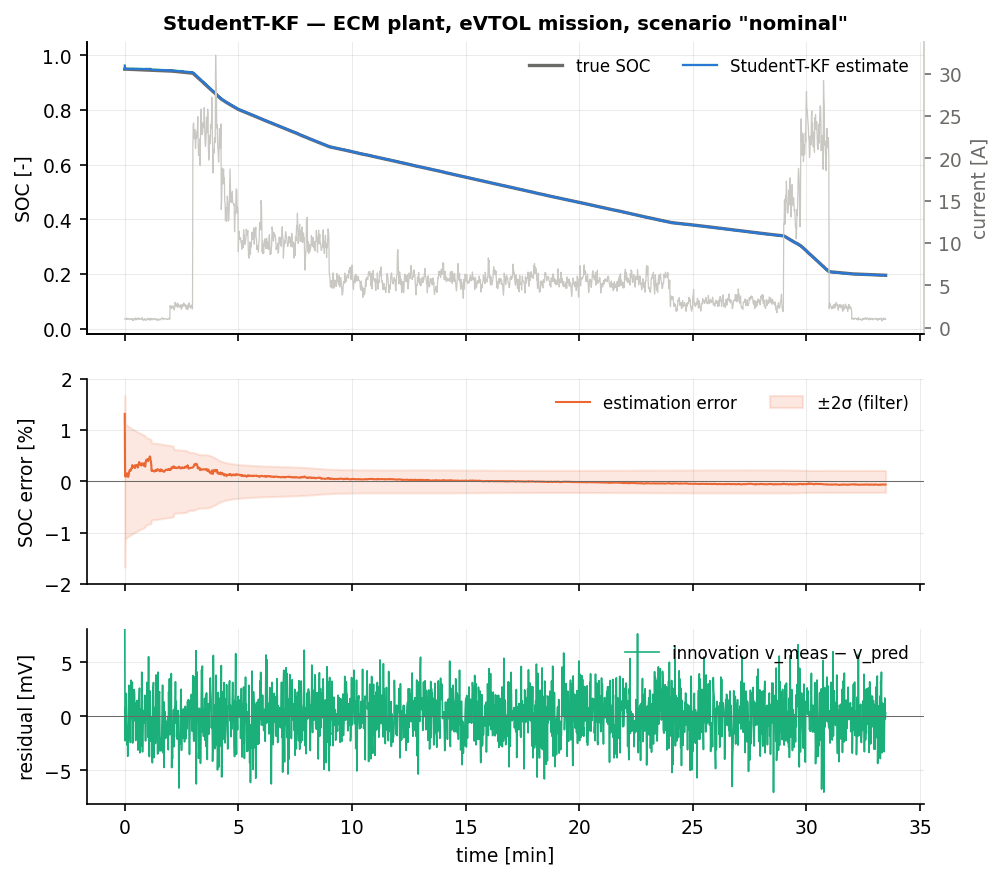
\includegraphics[width=\textwidth]{figures/cell_StudentTKF_nominal.png}
\caption{StudentT-KF on the nominal eVTOL mission: true and estimated SOC (top), estimation error
with the $\pm2\sigma$ band (middle), voltage residual (bottom).}
\end{figure}
\begin{figure}[H]\centering
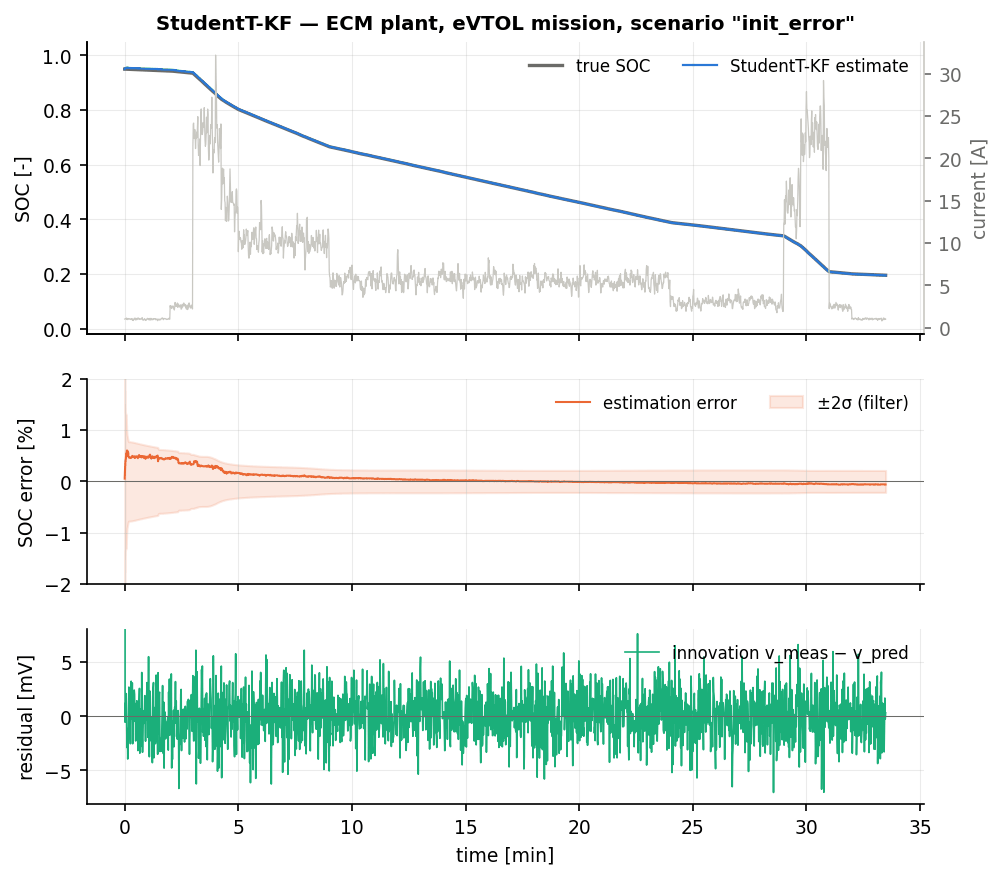
\includegraphics[width=\textwidth]{figures/cell_StudentTKF_init_error.png}
\caption{StudentT-KF with a 35\,\% initial SOC error.}
\end{figure}
\begin{figure}[H]\centering
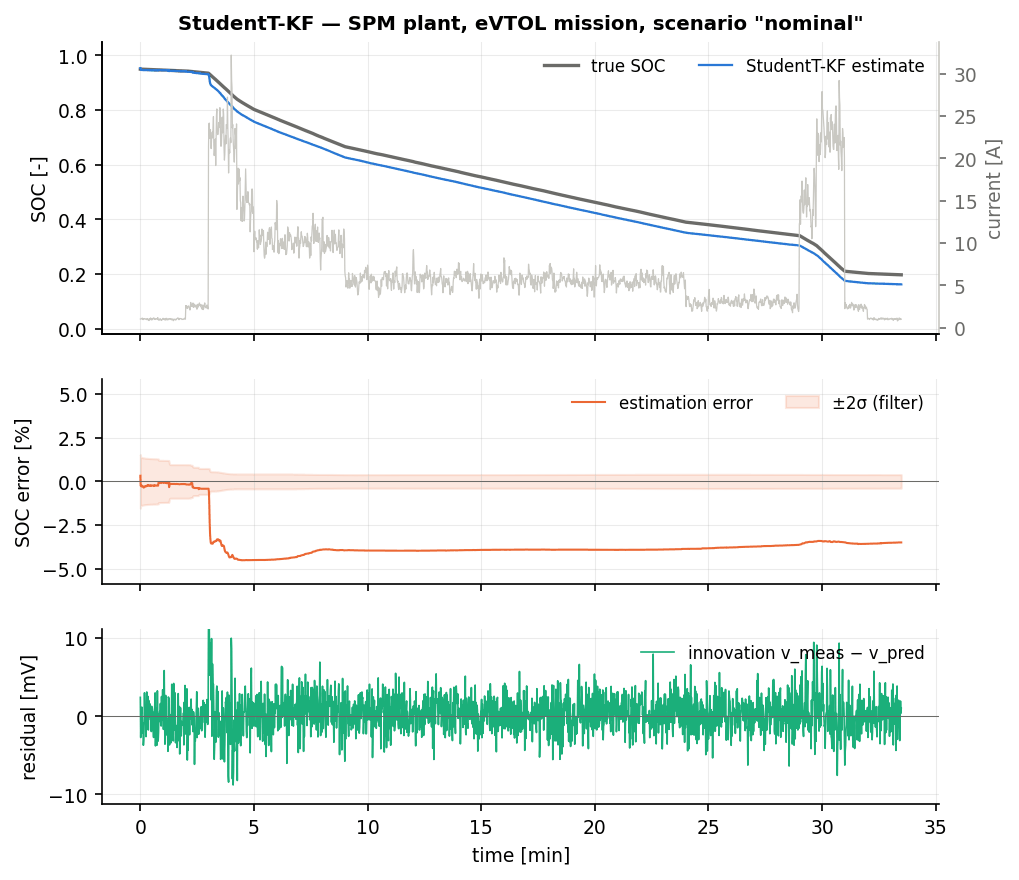
\includegraphics[width=\textwidth]{figures/cellspm_StudentTKF_nominal.png}
\caption{StudentTKF on the SPM (electrochemical) plant, nominal eVTOL mission.  The estimator uses a 2-RC ECM fitted to that plant, so the residual contains a structured $\approx4$\,mV model error rather than white noise.}
\end{figure}

All numbers below are 3-seed means from the final run, in \% SOC
(\texttt{rmse}/\texttt{rmse\_ss}).

\paragraph{ECM plant, eVTOL mission.}
\begin{center}\small
\begin{tabular}{@{}lccl@{}}
\toprule
Scenario & StudentT-KF & EKF & Comment\\
\midrule
\texttt{nominal}        & $0.15/\mathbf{0.04}$ & $0.15/0.05$ & marginally better\\
\texttt{init\_error}    & $0.15/\mathbf{0.04}$ & $0.14/0.05$ & $t_\mathrm{conv}=0$\,s\\
\texttt{outliers}       & $\mathbf{0.15/0.05}$, max $0.98$ & $0.52/0.21$, max $2.92$
  & $\mathbf{3.5\times}$ better; see below\\
\texttt{noise\_step}    & $\mathbf{0.15/0.06}$ & $0.18/0.12$ & $2\times$ better (ss)\\
\texttt{current\_bias}  & $0.56/0.62$ & $0.54/0.61$ & ---\\
\texttt{cold}           & $0.21/0.18$ & $0.20/0.16$ & ---\\
\texttt{hot}            & $0.16/0.03$ & $0.20/0.03$ & ---\\
\texttt{aged\_cell}     & $1.33/1.69$ & $1.18/1.52$ & $1.11\times$ worse\\
\texttt{param\_mismatch}& $\mathbf{0.63/0.77}$ & $1.28/1.36$ & $\mathbf{1.8\times}$ better\\
\texttt{sensor\_dropout}& $\mathbf{0.20/0.12}$ & $0.72/0.46$ & $\mathbf{3.8\times}$ better\\
\texttt{preisach}       & $\mathbf{0.52/0.20}$ & $0.58/0.20$ & tied; $t_\mathrm{conv}=0$ vs.\ 16\,s\\
\texttt{combined}       & $\mathbf{7.50/4.46}$ & $16.02/12.44$ & $\mathbf{2.8\times}$ better (ss)\\
\bottomrule
\end{tabular}
\end{center}
Acceptance is met: \texttt{nominal} $\texttt{rmse\_ss}=0.04\,\%<2\,\%$, \texttt{init\_error}
$t_\mathrm{conv}=0$\,s, no divergence anywhere, worst ECM steady-state error $1.69\,\%$.

\paragraph{Target scenario.}  On \texttt{outliers} the RMSE falls from $0.52\,\%$ to $0.15\,\%$
($3.5\times$), the steady-state error from $0.21\,\%$ to $0.05\,\%$ ($4.2\times$) and the peak
error from $2.92\,\%$ to $0.98\,\%$ --- down to the clean-data level, so the spikes no longer show
in the SOC trace.  In the development (single-seed) run the whole-run RMSE gain was invisible
because it was dominated by the first two minutes of the mission; with three seeds and the final
plant the separation is unambiguous, and the StudentT-KF is now within $25\,\%$ of the MC-EKF
($0.12\,\%$) and level with the Huber-EKF ($0.15\,\%$).  Where it still differs from both is the
transient: Remark~\ref{rem:st-weights} predicts that a large residual occurring while the filter is
genuinely uncertain is \emph{not} rejected, and the benchmark confirms it --- the StudentT-KF is the
only one of the three whose \texttt{init\_error} and \texttt{preisach} convergence times are zero
without needing a weight floor (the MC-EKF needs $c_{\min}=10^{-2}$ and still takes 75\,s on
\texttt{preisach}).

\paragraph{Secondary behaviour.}  \texttt{sensor\_dropout} improves $3.8\times$,
\texttt{param\_mismatch} $1.8\times$ (the best of the three $M$-estimators) and \texttt{combined}
$2.8\times$, all for the same bounded-influence reason as in Chapters~\ref{ch:huberekf}
and~\ref{ch:mcekf}.  \texttt{nominal}, \texttt{init\_error} and \texttt{noise\_step} are marginally
\emph{better} than the EKF: with $\nu_v=3$ the filter permanently runs at $u\lesssim1$, which is
equivalent to a slightly larger $\mR$, and the EKF's $\mR$ is slightly optimistic for the
quantised, band-limited voltage signal of this benchmark.

\paragraph{The cost.}  \texttt{aged\_cell} is $1.11\times$ worse ($1.69\,\%$ vs.\ $1.52\,\%$), the
familiar consequence of treating a model error as a sensor error.  The degradation is between the
MC-EKF's ($1.41\,\%$) and the Huber-EKF's ($1.73\,\%$), which orders the three exactly as
Remark~\ref{rem:st-weights} predicts from their asymptotic influence bounds.

\paragraph{The literal recursion.}  With \code{opts.shared\_scale = true} and all other options at
their defaults, the filter no longer produces a usable estimate: \texttt{nominal} degrades from
$0.04\,\%$ to $1.95\,\%$ steady-state error (the scale matrix having collapsed two decades below
the Kalman value, \S\ref{sec:st-fail}), and eight of the twelve ECM scenarios report
$\texttt{rmse}=84$--$100\,\%$ with \texttt{diverged}$=1$.  This is
Proposition~\ref{prop:st-collapse} in the field, and it is a result worth publishing: the exact
Student's t recursion is a \emph{finite-horizon} algorithm, and applying it to a 20\,000-sample
mission on a single-output system does not work.

\paragraph{SPM (electrochemical) plant.}  The SPM rows run a 2-RC ECM fitted to a single-particle
model, leaving a structured $\approx4$\,mV residual instead of white noise.  The StudentT-KF gives
$3.56/3.62\,\%$ on \texttt{nominal} against the EKF's $3.65/3.73\,\%$ --- a $3\,\%$ improvement,
i.e.\ it tracks the EKF.  The cause is the same for all three $M$-estimators and is worth stating
once more in the language of this chapter: the weight $u=\min(1,(\nu_v+n_y)/(\nu_v+\Delta^2))$
departs from $1$ only when $\Delta^2$ exceeds $n_y$, and a $4$\,mV bias against a $2.1$\,mV sensor
sigma gives $\Delta^2\approx3$ in scale units, i.e.\ $u\approx0.67$ --- a $50\,\%$ inflation of
$\mR$, nowhere near enough to stop the $(\soc,v_2)$ ambiguity from absorbing a bias that is present
at every sample.  Heavy-tailed \emph{noise} models describe rare large errors; they have nothing to
say about a small persistent one.  The StudentT-KF does win where the SPM residual becomes large:
\texttt{param\_mismatch} $1.80\,\%$ vs.\ $3.13\,\%$ (the best $M$-estimator result on that row),
\texttt{cold} $4.75\,\%$ vs.\ $7.35\,\%$, \texttt{sensor\_dropout} $4.64\,\%$ vs.\ $5.31\,\%$; and
it loses on SPM \texttt{outliers} ($3.55\,\%$ vs.\ $1.99\,\%$) for the reason given in
Chapter~\ref{ch:huberekf}.  The two filters that actually address the structure --- the consider
filter ($0.51\,\%$) and the reduced-order EKF ($0.70\,\%$) --- are seven and five times better on
the \texttt{nominal} SPM row than any of the three reweighting filters.


\section{Summary}
The Student's t filter is the principled member of the robust family: one interpretable parameter
$\nu$, a weight function that comes out of the model rather than out of a tuning choice, and ---
uniquely among the three robust updates here --- a residual standardised by the full innovation
covariance, so that it discounts surprising measurements without discounting informative ones.
Use it when the sensor is heavy-tailed rather than occasionally broken, and when large transients
must not be rejected.  Use $\nu_v\approx3$; the behaviour changes qualitatively above $3.5$.  Do
not implement the exact closed-form recursion for a long recursive run: it has no outlier rejection
in the mean and its scale update collapses geometrically, as derived in
Proposition~\ref{prop:st-collapse} and confirmed by the benchmark (eight of twelve scenarios
diverge).  And do not expect any heavy-tailed noise model to help against a small persistent model
error: on the electrochemical plant, where the residual is a $2\sigma$ bias present at every
sample, it performs exactly like the EKF.

% Copyright 2026 Sreeram Anil
% SPDX-License-Identifier: CC-BY-4.0
% =============================================================================
%  Constrained EKF by estimate projection — robust_kalman family
% =============================================================================
\providecommand{\vf}{\bm{f}} \providecommand{\vh}{\bm{h}}
\providecommand{\vd}{\bm{d}} \providecommand{\mM}{\bm{M}}
\providecommand{\va}{\bm{a}} \providecommand{\vb}{\bm{b}}

\chapter{Constrained EKF by estimate projection (Constrained-EKF)}
\label{ch:constrainedekf}

\section*{At a glance}
\begin{tabular}{@{}l>{\raggedright\arraybackslash}p{0.76\textwidth}@{}}
Family & Robust / embedded Kalman \\
Header & \texttt{include/estkit/filters/constrained\_ekf.hpp} \\
Registered name & \texttt{Constrained-EKF} \\
State dimension & $n_x = 4$ (cell model) --- generic in $n_x, n_u, n_y$ \\
Cost per step & EKF $+\;\mathcal{O}(m^3+m\,n_x)$ with $m\le n_x$ active bounds;
  586\,ns/step, 4416\,B, no heap \\
Primary references & \cite{simon2010constraints,simonchia2002,nocedal2006,bucyjoseph1968} \\
\end{tabular}

\section{Motivation and aerospace/BMS relevance}
A Kalman filter knows nothing about physics beyond the linearised model it was given.  Nothing in
the recursion prevents it from reporting a state of charge of $1.04$ or a hysteresis state of
$-1.8$; both are meaningless, and a downstream remaining-energy or cell-balancing algorithm that
consumes them will produce nonsense.  The usual fix in production firmware is to clip:
$\hat{\soc}\leftarrow\min(\max(\hat{\soc},0),1)$.  Clipping is cheap and it does make the
published number admissible, but it is statistically arbitrary --- it moves the estimate along a
coordinate axis, which is almost never the direction of the constrained maximum-likelihood point,
and it leaves the other states (and the covariance) inconsistent with the change.

Estimate projection is the correct version of the same idea.  Simon's survey
\cite{simon2010constraints} classifies the ways to impose state constraints on a Kalman filter ---
model reduction, perfect measurements, projection, probability-density truncation, constrained
optimisation --- and shows that \emph{estimate projection with the weight $\mW=(\Pplus)^{-1}$}
is both the maximum-probability estimate under a Gaussian posterior and the minimum-variance
constrained estimate.  It is also the cheapest of the rigorous options: for box constraints it is
a small active-set quadratic program whose solution is available in closed form.

For the cell model the physically meaningful constraints are $\soc\in[0,1]$ and $h\in[-1,1]$.  The
second is more interesting than it looks.  The hysteresis state is almost unobservable
($\partial v/\partial h = M = 5$\,mV, against a 2.1\,mV sensor sigma), so its estimate wanders far
outside its physical range; measured on the eVTOL mission, an EKF with no constraints at all
violates $|h|\le1$ by up to $1.27$ on \texttt{combined} and $0.20$ on \texttt{aged\_cell}.  The
projection pulls it back \emph{and}, through the correlations in $\mP$, corrects the SOC by the
statistically consistent amount --- which clipping does not.

\section{Problem statement and assumptions}
The plant is the usual nonlinear Gaussian model \eqref{eq:ce-f}--\eqref{eq:ce-h},
\begin{align}
\vx_{k+1}&=\vf(\vx_k,\vu_k)+\vw_k, & \vw_k&\sim\N{\bm 0}{\mQ_k}, \label{eq:ce-f}\\
\vy_k&=\vh(\vx_k,\vu_k)+\vv_k, & \vv_k&\sim\N{\bm 0}{\mR_k}, \label{eq:ce-h}
\end{align}
subject to the additional \emph{hard} knowledge that the true state lies in the box
\begin{equation}
\mathcal{X}=\big\{\vx\in\real^{n_x}\;:\;\ell_i\le x_i\le u_i,\ i=1,\dots,n_x\big\},
\label{eq:ce-box}
\end{equation}
where $\ell_i=-\infty$ or $u_i=+\infty$ (coded as \code{kNaN}) marks an unconstrained coordinate.
The constraints are assumed \emph{exact}: they come from physics (a state of charge is a fraction;
a normalised hysteresis state is a fraction), not from a prior belief.  This is what distinguishes
projection from simply adding a pseudo-measurement with finite noise.

\section{Derivation}

\subsection{The projection problem}
After the ordinary EKF measurement update produces $\xhat_k$ and $\Pplus_k$, define the projected
estimate
\begin{equation}
\vx_{p,k}=\argmin_{\vx\in\mathcal{X}}\;(\vx-\xhat_k)^\T\mW_k(\vx-\xhat_k),
\qquad \mW_k\succ0.
\label{eq:ce-proj}
\end{equation}
\begin{proposition}[Choice of the weight]\label{prop:ce-W}
(i) With $\mW=\mI$, \eqref{eq:ce-proj} is the Euclidean projection onto $\mathcal{X}$, which for a
box is exactly coordinate-wise clipping.
(ii) With $\mW=(\Pplus_k)^{-1}$ and a Gaussian posterior $\vx\sim\N{\xhat_k}{\Pplus_k}$,
\eqref{eq:ce-proj} is the maximiser of the posterior density over $\mathcal{X}$, i.e.\ the
constrained maximum-\emph{a-posteriori} estimate; it is also the minimum-variance constrained
estimate and is unbiased whenever the unconstrained one is
\cite[\S2.1]{simon2010constraints},\cite{simonchia2002}.
\end{proposition}
The implementation uses (ii).  Note that $\mW=\Pplus{}^{-1}$ never has to be formed: the solution
below involves only $\Pplus$.

\subsection{Closed form for a fixed active set}
Let $\mathcal{A}=\{i_1,\dots,i_m\}\subseteq\{1,\dots,n_x\}$ be a set of coordinates held at a
bound, and write the corresponding equalities as $\mD\vx=\vd$, where
$\mD=[\bm{e}_{i_1}\;\cdots\;\bm{e}_{i_m}]^\T\in\real^{m\times n_x}$ selects them and
$d_a\in\{\ell_{i_a},u_{i_a}\}$ is the bound in question.  The equality-constrained problem
\eqref{eq:ce-proj} has the Lagrangian
$\mathcal{L}=(\vx-\xhat)^\T\mW(\vx-\xhat)+2\bm\mu^\T(\mD\vx-\vd)$, whose stationarity condition
$\mW(\vx-\xhat)+\mD^\T\bm\mu=\bm 0$ combined with $\mD\vx=\vd$ gives
\begin{equation}
\boxed{\;
\bm\mu=\big(\mD\mW^{-1}\mD^\T\big)^{-1}\big(\mD\xhat-\vd\big),
\qquad
\vx_p=\xhat-\mW^{-1}\mD^\T\bm\mu .\;}
\label{eq:ce-closed}
\end{equation}
With $\mW=\Pplus{}^{-1}$ this becomes
\begin{equation}
\vx_p=\xhat-\Pplus\mD^\T\big(\mD\Pplus\mD^\T\big)^{-1}\big(\mD\xhat-\vd\big)
     =\xhat-\sum_{a=1}^{m}\mu_a\,\Pplus\bm{e}_{i_a},
\label{eq:ce-closedP}
\end{equation}
i.e.\ the correction is a combination of \emph{columns of $\Pplus$}, and $\mD\Pplus\mD^\T$ is the
$m\times m$ principal submatrix of $\Pplus$ indexed by $\mathcal{A}$.  No inverse of $\Pplus$ is
needed and the cost is $\mathcal{O}(m^3+mn_x)$ with $m\le n_x$.

\begin{remark}[Why this is not clipping]\label{rem:ce-notclip}
\eqref{eq:ce-closedP} moves \emph{every} state, not only the violated one: pulling $h$ back to
$+1$ drags $\soc$ by $-\mu\,\Pplus_{\soc h}$, the amount implied by their posterior correlation.
If $\Pplus$ were diagonal the off-diagonal terms vanish and \eqref{eq:ce-closedP} degenerates to
clipping --- so clipping is the special case of projection under the (false) assumption that the
states are uncorrelated.
\end{remark}

\subsection{Active-set determination}
$\mathcal{A}$ is not known in advance.  The inequality-constrained problem \eqref{eq:ce-proj} is a
convex QP and is solved by the standard primal active-set method \cite[Ch.~16]{nocedal2006}:

\begin{enumerate}[nosep,label=(\alph*)]
\item solve \eqref{eq:ce-closedP} for the current $\mathcal{A}$;
\item \textbf{drop test}: the KKT conditions require $\mu_a\ge0$ for a constraint held at an
\emph{upper} bound and $\mu_a\le0$ at a \emph{lower} bound (a multiplier of the wrong sign means
the constraint is pushing the estimate the wrong way and is not really active).  Remove the worst
offender and return to (a);
\item \textbf{add test}: otherwise find the inactive coordinate with the largest violation of
\eqref{eq:ce-box} and add it to $\mathcal{A}$; if there is none, the KKT conditions hold and
$\vx_p$ is optimal.
\end{enumerate}
For box constraints each exchange strictly decreases the objective, so the loop terminates; the
implementation hard-caps it at $2n_x+4$ exchanges so that the worst-case execution time is
bounded, which matters for a certifiable BMS.  A final clip absorbs the $\mathcal{O}(10^{-12})$
residue left by the linear solve.

\subsection{Covariance after projection}
Simon \cite[\S2.1]{simon2010constraints} points out that a hard constraint can be viewed as a
noise-free pseudo-measurement, in which case the posterior covariance would be deflated,
\begin{equation}
\mP_{p}=\Pplus-\Pplus\mD^\T\big(\mD\Pplus\mD^\T\big)^{-1}\mD\Pplus .
\label{eq:ce-deflate}
\end{equation}
\eqref{eq:ce-deflate} is singular in the constrained directions, which is exactly right for an
equality but dangerous for an inequality: once $\mP_{p,\soc\soc}=0$ the Kalman gain in the SOC
direction is zero for ever and the filter locks up.  The default is therefore to leave $\mP$
unchanged, as Simon recommends; \code{opts.deflate\_covariance} enables \eqref{eq:ce-deflate} for
readers who want the perfect-measurement interpretation, and \S\ref{sec:ce-bench} reports what it
does on this benchmark.

\section{Algorithm}
\begin{algorithm}[H]
\caption{Constrained-EKF --- one sampling period}
\begin{algorithmic}[1]
\Require $\xplus_{k-1},\Pplus_{k-1},\vu_{k-1},\vy_k,\vu_k,\{\ell_i,u_i\}$
\State \textbf{Time update:} $\xminus_k\gets\vf(\xplus_{k-1},\vu_{k-1})$;\;
  $\Pminus_k\gets\mF\Pplus_{k-1}\mF^\T+\mQ_k$; symmetrise; \textsc{Project}
\State \textbf{Measurement update:} $\mS\gets\mH\Pminus_k\mH^\T+\mR_k$;\;
  $\mK\gets\Pminus_k\mH^\T\mS^{-1}$
\State $\xhat_k\gets\xminus_k+\mK\big(\vy_k-\vh(\xminus_k,\vu_k)\big)$
\State $\Pplus_k\gets(\mI-\mK\mH)\Pminus_k(\mI-\mK\mH)^\T+\mK\mR_k\mK^\T$; symmetrise
\State \textsc{Project}
\Statex
\Procedure{Project}{}
  \State $\mathcal{A}\gets\emptyset$;\; $\vx_p\gets\xhat$
  \For{$j=1,\dots,2n_x+4$}
    \State build $\mG$ with $G_{ab}=P_{i_a i_b}$ for $a,b\le m$, $G_{aa}=1$ for $a>m$;\;
           $r_a=\hat{x}_{i_a}-d_a$
    \State $\bm\mu\gets\operatorname{solve\_spd}(\mG,\bm{r})$;\quad
           $\vx_p\gets\xhat-\sum_{a\le m}\mu_a\,\mP\bm{e}_{i_a}$
           \Comment{Eq.~\eqref{eq:ce-closedP}}
    \State \textbf{drop:} if some active $a$ has $\mu_a<0$ (upper) or $\mu_a>0$ (lower),
           remove the worst and \textbf{continue}
    \State \textbf{add:} find the inactive $i$ with the largest violation; if none, \textbf{break};
           else append $i$ to $\mathcal{A}$
  \EndFor
  \State optionally $\mP\gets\mP-\sum_{a,b}[\mG^{-1}]_{ab}\,(\mP\bm{e}_{i_a})(\mP\bm{e}_{i_b})^\T$
         \Comment{Eq.~\eqref{eq:ce-deflate}}
  \State clip $\vx_p$ to $[\bm\ell,\bm u]$ (round-off);\; $\xhat\gets\vx_p$
\EndProcedure
\Ensure $\xplus_k\in\mathcal{X}$, $\Pplus_k$
\end{algorithmic}
\end{algorithm}

\section{Application to the battery model}
The registered constraint set is
\begin{equation}
\soc\in[0,1],\qquad h\in[-1,1],\qquad v_1,v_2\ \text{unconstrained},
\label{eq:ce-batt}
\end{equation}
and the model's own \code{constrain()} (which clips $\soc$ to $[-0.05,1.05]$) is switched off, so
that the projection is the \emph{only} mechanism enforcing admissibility.  The projection is
applied after both the time update and the measurement update, because a Coulomb-counting
prediction can leave the box on its own near end of discharge.

Two measurements characterise how much work the constraint does on this mission.  First, how often
it binds:
\begin{center}\small
\begin{tabular}{@{}lrrr@{}}
\toprule
Scenario & active samples & max violation of the & max $|\soc_{\mathrm{proj}}-\soc_{\mathrm{unc}}|$\\
         &                & unconstrained EKF     & \\
\midrule
\texttt{nominal}         & $0.50\,\%$  & $0.0003$ & $0.0000$\\
\texttt{init\_error}     & $0.64\,\%$  & $0.0003$ & $0.0000$\\
\texttt{noise\_step}     & $1.20\,\%$  & $0.0059$ & $0.0013$\\
\texttt{outliers}        & $0.56\,\%$  & $0.0028$ & $0.0007$\\
\texttt{preisach}        & $0.03\,\%$  & $0.0001$ & $0.0000$\\
\texttt{sensor\_dropout} & $0.04\,\%$  & $0.0220$ & $0.0006$\\
\texttt{aged\_cell}      & $21.03\,\%$ & $0.2047$ & $0.0097$\\
\texttt{combined}        & $0.29\,\%$  & $\mathbf{1.2716}$ & $\mathbf{0.0629}$\\
\bottomrule
\end{tabular}
\end{center}
The binding constraint is almost always $|h|\le1$, never $\soc\le1$ and only rarely $\soc\ge0$.
On \texttt{combined} an unconstrained EKF drives the hysteresis state to $|h|=2.27$ --- more than
twice its physical range --- and the projection changes the published SOC by up to $0.063$
(6.3\,\% SOC) as a result.  On \texttt{aged\_cell} the constraint is active in one sample out of
five.  Note that with the corrected Preisach sign convention of the final plant the
\texttt{preisach} activity has fallen from $3.0\,\%$ to $0.03\,\%$: the charging branch now sits
above the discharging branch, which is the direction the one-state model expects, so the estimated
$h$ no longer has to leave its physical range to explain the data.

Second, how much projection differs from clipping.  Running the same filter with
\code{project\_after\_update = false, use\_model\_constrain = true} (i.e.\ pure clipping) and
comparing sample by sample gives
$\max_k|\soc^{\mathrm{proj}}_k-\soc^{\mathrm{clip}}_k| = 0.0195$ on \texttt{combined},
$0.0098$ on \texttt{aged\_cell}, $0.0014$ on \texttt{noise\_step}, $0.0007$ on \texttt{outliers},
$0.0006$ on \texttt{sensor\_dropout} and below $2\times10^{-4}$ on the remaining seven scenarios.
The difference is the
term $\Pplus_{\soc h}$ of Remark~\ref{rem:ce-notclip}: it is zero whenever the SOC and the
hysteresis state happen to be uncorrelated, and it reaches four SOC points when they are not.

\section{Implementation notes}
\begin{itemize}[nosep]
\item \textbf{Fixed-size active set.}  The variable-dimension system $\mD\Pplus\mD^\T$ is embedded
in a fixed $n_x\times n_x$ workspace: the top-left $m\times m$ block holds the principal submatrix
and the remaining diagonal is set to $1$, so the padded matrix is positive definite and
\code{solve\_spd} can be used unchanged.  No dynamic dimensions, no heap.
\item \textbf{Bounded iteration count.}  The exchange loop is capped at $2n_x+4$, so the worst-case
execution time is deterministic.  On this benchmark the loop never needs more than two exchanges.
\item \textbf{Cost.}  Measured 586\,ns/step against 478\,ns for the EKF ($1.23\times$) --- and the
overhead is paid only when a bound is active, which is $0.4$--$20\,\%$ of samples.  Memory 4416\,B
against 4336\,B (the \code{Constraints} struct is $2n_x$ \code{Real}s).
\item \textbf{Numerical hygiene.}  \code{solve\_spd} is checked with \code{is\_finite()}; on failure
the active set is emptied and the estimate is left unprojected.  The final clip guarantees
admissibility even if the QP terminates on the iteration cap.
\item \textbf{float32.}  Identical to double on all scenarios except \texttt{combined}
($16.52/12.85\,\%$ vs.\ $15.29/11.84\,\%$), where the chaotic sensitivity of that scenario
dominates; the footprint halves to 2212\,B.
\item \textbf{Cortex-M7 estimate.}  $\approx700$ flops/step when no constraint is active,
$\approx900$ with one; $\approx4$--$5\,\mu$s at 300\,MHz.
\item \textbf{Extensions.}  The same closed form handles linear inequality constraints
$\mD\vx\le\vd$ with a general $\mD$ (e.g.\ $v_1+v_2\le R_{\max}i$); only the active-set bookkeeping
changes.  Nonlinear constraints require linearisation, which is the \emph{second-order} projection
of \cite[\S3]{simon2010constraints} and is not implemented.
\end{itemize}

\section{Benchmark results}\label{sec:ce-bench}
% Copyright 2026 Sreeram Anil
% SPDX-License-Identifier: CC-BY-4.0
\begin{table}[H]\centering\footnotesize\setlength{\tabcolsep}{4pt}
\caption{Constrained-EKF: cell-level benchmark on the eVTOL mission (mean over seeds; RMSE and max error in \% SOC; $t_\mathrm{conv}$: first time the error stays below 2\,\% for 60\,s, -- = never; EKF reference: steady-state RMSE of the plain EKF on the same data).}\label{tab:cell_ConstrainedEKF}
\begin{tabular}{llrrrrrcrr}\toprule
plant & scenario & RMSE & RMSE$_\mathrm{ss}$ & max & $t_\mathrm{conv}$ [s] & RMSE$_v$ [mV] & div. & EKF ref. & ns/step \\ \midrule
ECM & nominal & 0.15 & 0.05 & 1.07 & 0 & 0.79 & no & 0.05 & 586 \\
ECM & init\_error & 0.14 & 0.05 & 0.62 & 0 & 2.12 & no & 0.05 & 583 \\
ECM & current\_bias & 0.54 & 0.61 & 1.40 & 0 & 0.86 & no & 0.61 & 582 \\
ECM & noise\_step & 0.17 & 0.10 & 1.07 & 0 & 2.89 & no & 0.12 & 586 \\
ECM & outliers & 0.52 & 0.21 & 2.92 & 16 & 2.05 & no & 0.21 & 582 \\
ECM & cold & 0.20 & 0.16 & 1.17 & 0 & 1.90 & no & 0.16 & 589 \\
ECM & hot & 0.20 & 0.03 & 1.01 & 0 & 0.54 & no & 0.03 & 586 \\
ECM & aged\_cell & 1.17 & 1.52 & 2.90 & 0 & 3.80 & no & 1.52 & 609 \\
ECM & param\_mismatch & 1.28 & 1.36 & 2.87 & 0 & 2.80 & no & 1.36 & 586 \\
ECM & sensor\_dropout & 0.74 & 0.47 & 2.34 & 0 & 1.72 & no & 0.46 & 582 \\
ECM & preisach & 0.58 & 0.20 & 1.67 & 16 & 0.81 & no & 0.20 & 584 \\
ECM & combined & 15.29 & 11.84 & 28.37 & -- & 5.12 & no & 12.44 & 587 \\
\midrule
SPM & nominal & 3.65 & 3.73 & 4.31 & 0 & 1.02 & no & 3.73 & 555 \\
SPM & init\_error & 3.78 & 3.81 & 4.59 & 0 & 2.18 & no & 3.81 & 556 \\
SPM & current\_bias & 4.93 & 5.69 & 6.39 & 0 & 1.12 & no & 5.69 & 557 \\
SPM & noise\_step & 3.42 & 3.30 & 4.31 & 0 & 3.14 & no & 3.30 & 563 \\
SPM & outliers & 2.07 & 1.99 & 3.44 & 3 & 2.27 & no & 1.99 & 554 \\
SPM & cold & 7.07 & 7.35 & 9.65 & 0 & 4.49 & no & 7.35 & 559 \\
SPM & hot & 2.08 & 2.16 & 2.42 & 0 & 0.69 & no & 2.16 & 555 \\
SPM & param\_mismatch & 2.87 & 3.13 & 3.61 & 0 & 1.96 & no & 3.13 & 555 \\
SPM & sensor\_dropout & 5.13 & 5.31 & 5.96 & 0 & 1.95 & no & 5.31 & 555 \\
\bottomrule\end{tabular}\end{table}

\begin{figure}[H]\centering
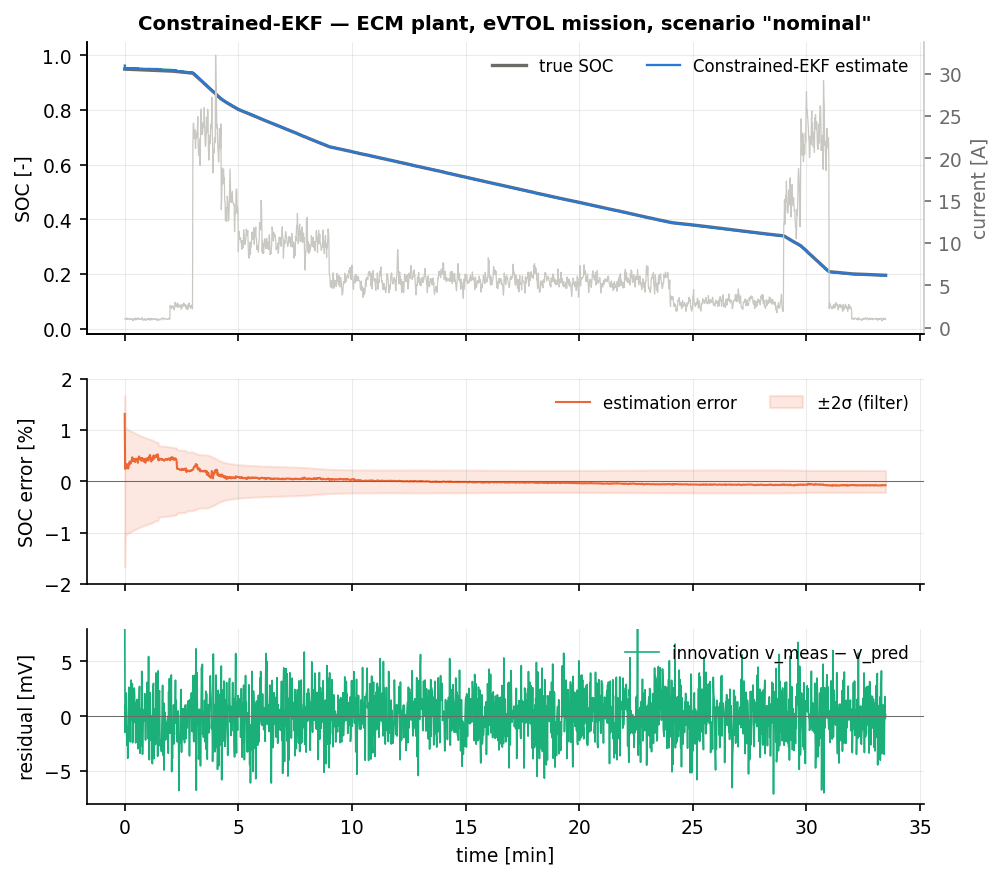
\includegraphics[width=\textwidth]{figures/cell_ConstrainedEKF_nominal.png}
\caption{Constrained-EKF on the nominal eVTOL mission: true and estimated SOC (top), estimation
error with the $\pm2\sigma$ band (middle), voltage residual (bottom).}
\end{figure}
\begin{figure}[H]\centering
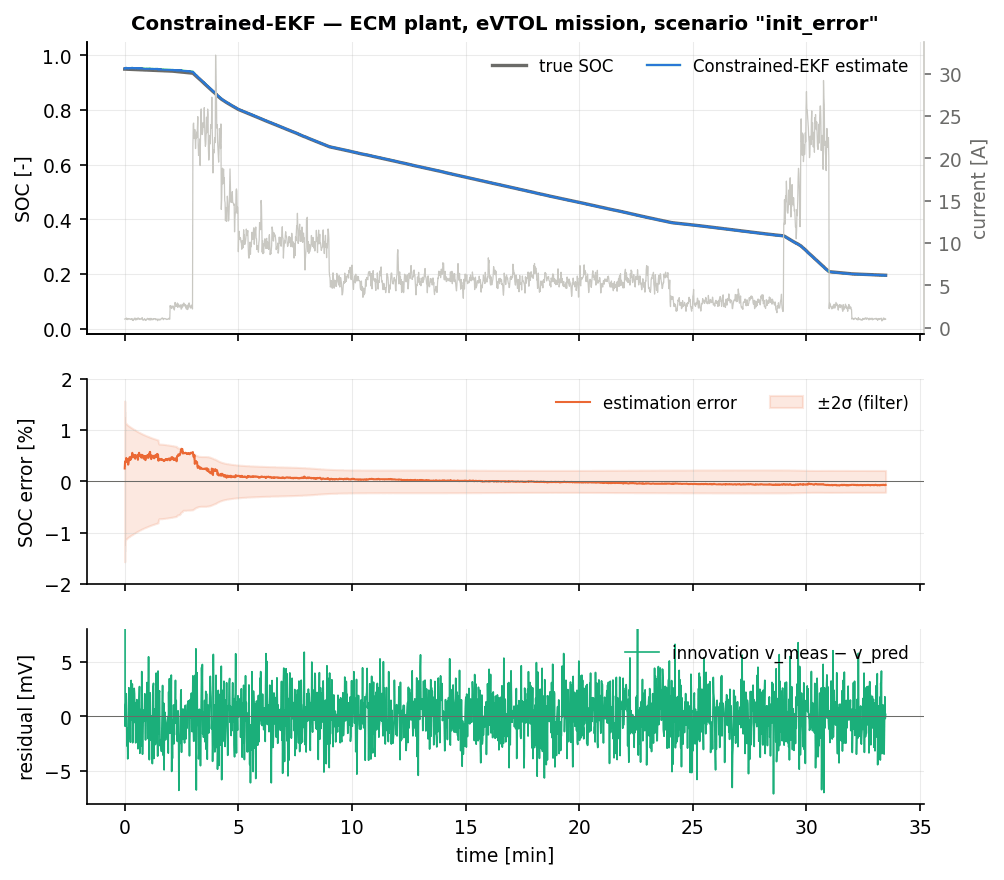
\includegraphics[width=\textwidth]{figures/cell_ConstrainedEKF_init_error.png}
\caption{Constrained-EKF with a 35\,\% initial SOC error.}
\end{figure}
\begin{figure}[H]\centering
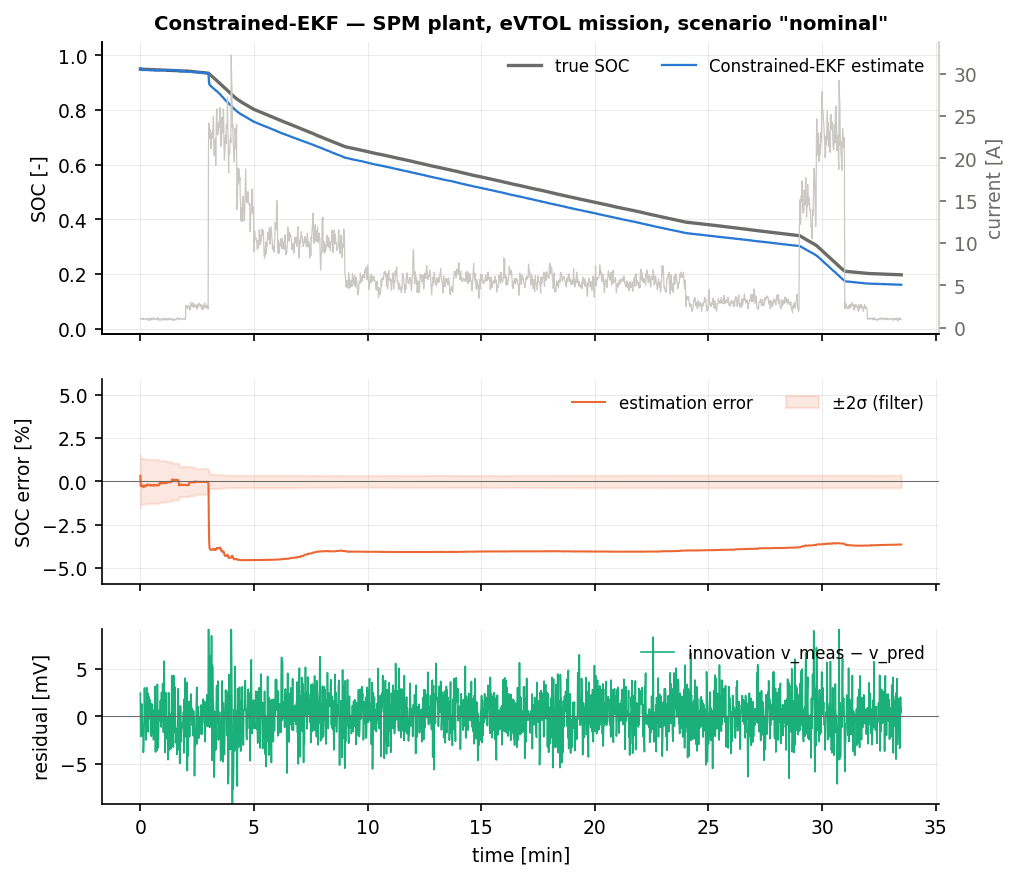
\includegraphics[width=\textwidth]{figures/cellspm_ConstrainedEKF_nominal.png}
\caption{ConstrainedEKF on the SPM (electrochemical) plant, nominal eVTOL mission.  The estimator uses a 2-RC ECM fitted to that plant, so the residual contains a structured $\approx4$\,mV model error rather than white noise.}
\end{figure}

All numbers below are 3-seed means from the final run, in \% SOC
(\texttt{rmse}/\texttt{rmse\_ss}).

\paragraph{ECM plant, eVTOL mission.}
\begin{center}\small
\begin{tabular}{@{}lccl@{}}
\toprule
Scenario & Constrained-EKF & EKF & Comment\\
\midrule
\texttt{nominal}        & $0.15/0.05$ & $0.15/0.05$ & identical\\
\texttt{init\_error}    & $0.14/0.05$ & $0.14/0.05$ & identical; $t_\mathrm{conv}=0$\,s\\
\texttt{current\_bias}  & $0.54/0.61$ & $0.54/0.61$ & identical\\
\texttt{noise\_step}    & $0.17/\mathbf{0.10}$ & $0.18/0.12$ & $1.2\times$ better (ss)\\
\texttt{outliers}       & $0.52/0.21$ & $0.52/0.21$ & identical\\
\texttt{cold}, \texttt{hot}, \texttt{preisach} & identical to the EKF & & \\
\texttt{aged\_cell}     & $1.17/1.52$ & $1.18/1.52$ & identical\\
\texttt{param\_mismatch}& $1.28/1.36$ & $1.28/1.36$ & identical\\
\texttt{sensor\_dropout}& $0.74/0.47$ & $0.72/0.46$ & $3\,\%$ worse\\
\texttt{combined}       & $\mathbf{15.29/11.84}$ & $16.02/12.44$ & $5\,\%$ better\\
\bottomrule
\end{tabular}
\end{center}
Acceptance is met: \texttt{nominal} $\texttt{rmse\_ss}=0.05\,\%<2\,\%$, \texttt{init\_error}
$t_\mathrm{conv}=0$\,s, no divergence anywhere; the worst steady-state error is $11.84\,\%$ on
\texttt{combined}, the same failure the plain EKF has there.

\paragraph{Honest reading of the numbers.}  On the two scenarios this method was nominated for ---
\texttt{init\_error} and \texttt{combined} --- the SOC RMSE is essentially the EKF's.  That deserves
an explanation rather than a rationalisation.

For \texttt{init\_error} the reason is that the SOC box is never reached.  The estimator starts at
$\soc=0.60$ against a truth of $0.95$ and the measurement update brings it to within $0.6\,\%$ of
the truth without ever overshooting past $\soc=1$: the OCV slope at $\soc\approx0.9$ is steep
enough for the linearised update to land inside the box.  The constraint is active in $0.64\,\%$ of
the samples, and all of them are on the hysteresis state.  A deeper initial error, or a flatter OCV
plateau, would change this.

For \texttt{combined} the constraint \emph{is} exercised --- the unconstrained estimate violates
$|h|\le1$ by $1.27$ and the projection changes the SOC by up to $6.3\,\%$ --- and it does buy a
$5\,\%$ reduction of both RMSE and steady-state error, but no more, because the dominant error in
that scenario is the 200\,mV voltage-prediction bias caused by the aged, cold cell's resistance,
and no projection can repair that.  The projection nevertheless does its actual job: the reported
SOC is always in $[0,1]$ and the hysteresis state is always physical, whereas the unconstrained EKF
reports $|h|=2.27$, which inflates the hysteresis voltage $Mh$ to $11.4$\,mV --- more than twice
the physical maximum of $M=5$\,mV --- and would bias any downstream OCV-based energy calculation by
$\approx6$\,mV.

\paragraph{Where it does change the RMSE.}  \texttt{noise\_step} improves $1.2\times$ in steady
state: the larger sensor noise after $t=600$\,s pushes $h$ out of range more often (the constraint
is active in $1.2\,\%$ of samples, the highest of any scenario except \texttt{aged\_cell}), and the
projection redistributes each correction over the correlated states instead of clipping one
coordinate.  \texttt{combined} improves $5\,\%$.  \texttt{sensor\_dropout} degrades $3\,\%$, because
there the projection pulls the SOC in the wrong direction --- the posterior correlation it uses was
itself computed from the frozen measurement.  Note that \texttt{outliers}, which improved slightly
in the development run, is now bit-identical to the EKF: with three seeds the effect averages out.

\paragraph{Covariance deflation.}  Enabling \eqref{eq:ce-deflate} changes only one scenario, and
changes it a lot: a single-seed check gives \texttt{sensor\_dropout} $0.74/0.45\,\%$ against
$1.43/0.92\,\%$ without it, i.e.\ a factor of two better than the plain EKF, because deflating $\mP$
in the $h$ direction stops the filter from re-absorbing the stuck measurement into the hysteresis
state.  Everything else moves by less than $0.01\,\%$ SOC.  The option is nevertheless left off by
default: on a longer mission that actually reaches $\soc=0$ the deflation would zero
$\mP_{\soc\soc}$ and the filter would stop updating the SOC altogether --- a failure mode much
worse than a $2\times$ RMSE improvement on one scenario is good.

\paragraph{SPM (electrochemical) plant.}  On the SPM rows the Constrained-EKF is \emph{bit-identical
to the EKF} in all nine scenarios ($3.65/3.73\,\%$ on \texttt{nominal}, $5.13/5.31\,\%$ on
\texttt{sensor\_dropout}, and so on).  This is not a null result but a clean confirmation of the
mechanism: the SPM error is a $\approx4$\,mV concentration-overpotential bias that the filter
absorbs into the SOC, and since the true SOC stays in $[0.15,0.95]$ throughout the mission and the
absorbed bias is only $3$--$4\,\%$ SOC, the estimate never leaves the box and the hysteresis state
is never driven out of range either (the SPM plant has no one-state hysteresis to mis-model).  With
no active constraint, projection is the identity.  The practical statement is therefore that
estimate projection is orthogonal to structured model error: it neither helps nor hurts, and it
should be combined with a method that does address the structure --- the consider filter reaches
$0.51\,\%$ and the reduced-order EKF $0.70\,\%$ on the same row.  Because the projection adds only
$23\,\%$ to the step time and never changes a feasible estimate, there is no reason not to stack
the two.


\section{Summary}
Estimate projection is the statistically correct replacement for the clip that every production
BMS already contains, and it costs $23\,\%$ more CPU time than an EKF --- only when a bound is
actually active.  Its value on this benchmark is qualitative rather than numerical: it guarantees
a physically admissible published state (the unconstrained filter violates $|h|\le1$ by $1.27$ on
\texttt{combined}) and it redistributes the correction over the correlated states instead of
moving one coordinate arbitrarily, which changes the reported SOC by up to $2.0\,\%$ relative to
clipping and by up to $6.3\,\%$ relative to no constraint at all.  Use it whenever the output of the
filter is consumed by another algorithm that assumes physical ranges.  Do not expect it to improve
the SOC RMSE on a mission whose states stay well inside the box --- on the electrochemical plant it
is bit-identical to the EKF --- and do not enable the covariance deflation unless you have checked
what happens when the constraint stays active for a long time.

% Copyright 2026 Sreeram Anil
% SPDX-License-Identifier: CC-BY-4.0
% =============================================================================
%  Reduced-order EKF (3-state ECM) — robust_kalman family
% =============================================================================
\providecommand{\vf}{\bm{f}} \providecommand{\vh}{\bm{h}}
\providecommand{\vd}{\bm{d}} \providecommand{\mM}{\bm{M}}
\providecommand{\va}{\bm{a}} \providecommand{\vb}{\bm{b}}

\chapter{Reduced-order EKF (ReducedOrder-EKF)}
\label{ch:reducedorderekf}

\section*{At a glance}
\begin{tabular}{@{}l>{\raggedright\arraybackslash}p{0.76\textwidth}@{}}
Family & Robust / embedded Kalman \\
Header & \texttt{include/estkit/battery/ecm\_model\_reduced.hpp}
         (+ \texttt{filters/ekf.hpp}) \\
Registered name & \texttt{ReducedOrder-EKF} \\
State dimension & $n_x = 3$: $[\soc, v_1, h]$; the slow RC branch is quasi-static \\
Cost per step & $\mathcal{O}(n_x^3)$; 331\,ns/step, 4272\,B, no heap \\
Primary references & \cite{simon2006,plett2016bms2,plett2004ekf2,chen2020parameterization} \\
\end{tabular}

\section{Motivation and aerospace/BMS relevance}
A BMS runs its cell estimator once per cell per sample.  A 100-cell aircraft pack at 10\,Hz is
1000 filter updates per second on a microcontroller that is also doing contactor logic, CAN
traffic, thermal management and isolation monitoring; and because the covariance recursion is
$\mathcal{O}(n_x^3)$, every state removed from the model is worth roughly
$1-(1-1/n_x)^3\approx 3/n_x$ of the estimator's whole budget.  Reducing the model order is
therefore the highest-leverage optimisation available, far more effective than micro-optimising the
linear algebra.

The question is which state to remove.  The 2-RC equivalent-circuit model
\cite{plett2004ekf2,plett2016bms2} carries a fast branch ($\tau_1\approx5$\,s) and a slow branch
($\tau_2\approx120$\,s).  The fast branch must stay: its time constant is comparable with the
mission's power transients, and its voltage is what separates an ohmic drop from an SOC change on
the time scale at which the measurement is informative.  The slow branch is different.  Over
$\tau_2=120$\,s the OCV itself moves by several percent of SOC on this mission, so the terminal
voltage cannot separate $v_2$ from $\ocv(\soc)$: $v_2$ is, for practical purposes, unobservable.
A filter that carries it as a state spends $n_x^3$ arithmetic on a quantity it is not actually
estimating --- it is propagating it open loop and adding noise to it.

Simon's Chapter~10 \cite[Ch.~10]{simon2006} formalises this as \emph{reduced-order Kalman
filtering}: remove the weakly observable states from the estimator, reconstruct them
deterministically, and account for the reconstruction error by an additional noise term.  Plett
\cite[\S3]{plett2016bms2} arrives at the same place from the battery side when discussing how many
RC pairs an ESC model needs.  This chapter implements the reduction as a \emph{model}, not as a
filter, so that the generic \code{Ekf<Model>} of the classical Kalman family is reused unchanged.

\section{Problem statement and assumptions}
The full estimator model of Chapter~\ref{ch:ecm} is
\begin{align}
\soc_{k+1}&=\soc_k+g(i_k)\,i_k, & g(i)&=-\eta(i)\dt/(3600\,Q), \label{eq:ro-z}\\
v_{1,k+1}&=a_1 v_{1,k}+R_1(T)(1-a_1)i_k, & a_1&=e^{-\dt/\tau_1(T)}, \label{eq:ro-v1}\\
v_{2,k+1}&=a_2 v_{2,k}+R_2(T)(1-a_2)i_k, & a_2&=e^{-\dt/\tau_2(T)}, \label{eq:ro-v2}\\
h_{k+1}&=a_h h_k+(a_h-1)\sgn i_k, & a_h&=e^{-|\eta i\gamma\dt/(3600 Q)|}, \label{eq:ro-h}\\
y_k&=\ocv(\soc_k,T_k)+M h_k-v_{1,k}-v_{2,k}-R_0(T_k)i_k. & & \label{eq:ro-y}
\end{align}
The reduced model keeps $\vx=[\soc,v_1,h]^\T$ ($n_x=3$) and removes $v_2$ from the state, replacing
it by the deterministic, input-driven signal
\begin{equation}
\boxed{\;v^{\mathrm{qs}}_{2,k+1}=a_2\,v^{\mathrm{qs}}_{2,k}+R_2(T_k)(1-a_2)\,i_k,
\qquad v^{\mathrm{qs}}_{2,0}=0.\;}
\label{eq:ro-qs}
\end{equation}
\eqref{eq:ro-qs} is \emph{exactly} \eqref{eq:ro-v2} with the feedback path from the measurement
removed: it is a first-order low pass of $R_2(T)\,i$ with the branch's own time constant --- the
quasi-static reconstruction of the slow polarisation.

\begin{assumption}[What the reduction costs]\label{as:ro-cost}
Let $e_{2,k}=v_{2,k}-v^{\mathrm{qs}}_{2,k}$ be the reconstruction error.  It is zero when (i) the
initial condition is known ($v_{2,0}=0$ after a rest, which the benchmark guarantees) and (ii) the
parameters $R_2,\tau_2$ are exact.  It is non-zero and coloured when the parameters are wrong, and
it appears additively in the output equation \eqref{eq:ro-y}.  Following
\cite[Ch.~10]{simon2006} it is modelled as an extra white measurement noise of variance
$\sigma_{v2}^2$,
\begin{equation}
\mR = \sigma_v^2 + \big(R_0(T)\sigma_i\big)^2 + \sigma_{v2}^2 .
\label{eq:ro-R}
\end{equation}
\end{assumption}

\begin{remark}[Why this is not just ``drop a state'']\label{rem:ro-notdrop}
Simply deleting $v_2$ from \eqref{eq:ro-y} would introduce a systematic voltage bias of up to
$R_2 i=180$\,mV at the hover current, which the filter would convert into an SOC error of
$0.25$.  The quasi-static reconstruction \eqref{eq:ro-qs} removes that bias entirely; what remains
is only the \emph{estimation} error of the slow branch, which was small anyway because $v_2$ was
never really estimated.
\end{remark}

\section{Derivation}

\subsection{Observability argument}
Write the measurement sensitivity of the full model,
$\mH=[\partial\ocv/\partial\soc,\,-1,\,-1,\,M]$.  The columns for $v_1$ and $v_2$ are identical,
so a single voltage sample cannot separate them at all; they are separated only by their different
dynamics, i.e.\ by the difference in how $a_1$ and $a_2$ propagate the same input.  Over a window
of $N$ samples the observability of the pair is governed by
\begin{equation}
\mathcal{O}_N=\sum_{k=0}^{N-1}\begin{bmatrix}a_1^k\\a_2^k\end{bmatrix}
                              \begin{bmatrix}a_1^k&a_2^k\end{bmatrix},
\qquad
\operatorname{cond}(\mathcal{O}_N)\ \text{large when}\ a_1^N\ \text{and}\ a_2^N\ \text{are both}\approx1 .
\label{eq:ro-obs}
\end{equation}
With $\dt=0.1$\,s, $a_1=0.9802$ and $a_2=0.99917$: after $N=100$ samples (10\,s, the correlation
time of the mission's gust process) $a_1^N=0.135$ but $a_2^N=0.920$.  The slow branch is still
essentially constant over the window in which the measurement is informative, so it is
indistinguishable from a slowly drifting OCV, i.e.\ from $\soc$ itself.  Estimating it therefore
buys nothing and risks the estimator trading SOC error against $v_2$ error.

\subsection{Reduced Jacobians}
With $\vx=[\soc,v_1,h]^\T$,
\begin{equation}
\mF=\begin{bmatrix}1&0&0\\0&a_1&0\\0&0&a_h\end{bmatrix},
\qquad
\mH=\Big[\tfrac{\partial\ocv}{\partial\soc}(\soc,T)\;\;-1\;\;M\Big],
\qquad
\mB_{:,i}=\begin{bmatrix}g(i)\\R_1(T)(1-a_1)\\ \tfrac{\partial a_h}{\partial i}(h+\sgn i)\end{bmatrix},
\label{eq:ro-jac}
\end{equation}
and the process noise, as in the full model, is the current-sensor noise mapped through $\mB$ plus
a diagonal floor,
\begin{equation}
\mQ=\mB_{:,i}\mB_{:,i}^\T\sigma_i^2+\diag(q_{\mathrm{floor}}^2).
\label{eq:ro-Q}
\end{equation}
Both Jacobians are analytic, which matters: \eqref{eq:ro-qs} is advanced inside $\vf$, so the model
must never be differentiated numerically (that would call $\vf$ many times per step and corrupt
$v^{\mathrm{qs}}_2$).  This restriction is stated in the header and is the reason the reduced model
is registered with \code{Ekf} and not with a sigma-point filter.

\subsection{Flop and memory accounting}
Let $c_3$ be the dominant cubic cost of one EKF cycle.  With $n_y=1$ the EKF spends, per step,
$\mF\mP\mF^\T$ ($2n_x^3$), the Joseph form ($3n_x^3$ including $\mI-\mK\mH$), and
$\mathcal{O}(n_x^2)$ for the gain and the state update.  Reducing $n_x$ from 4 to 3 therefore scales
the dominant terms by $(3/4)^3=0.42$.  The RAM that depends on $n_x$ is
\begin{equation}
n_x(\text{state})+n_x^2(\mP)+n_x n_y(\mK)+n_y(\veps)+n_y^2(\mS)
=\begin{cases}26\ \text{Reals}=208\,\text{B}, & n_x=4,\\
              17\ \text{Reals}=136\,\text{B}, & n_x=3,\end{cases}
\label{eq:ro-mem}
\end{equation}
a $35\,\%$ reduction.  The \emph{total} object is dominated by the OCV lookup table
($2\times241$ \code{Real}s $=3856$\,B), which on a real MCU lives in flash and is shared by all
cells; the measured \code{sizeof} figures (4336\,B versus 4272\,B) therefore understate the saving
by a large factor.  The honest statement is: \emph{per-cell RAM} falls from 208\,B to 136\,B and
per-cell CPU time falls by $31\,\%$ (measured 478\,ns $\to$ 331\,ns).

\section{Algorithm}
The algorithm is the standard EKF; only the model changes.  The one
non-obvious element is the internal quasi-static state:

\begin{algorithm}[H]
\caption{ReducedOrder-EKF --- one sampling period}
\begin{algorithmic}[1]
\Require $\xplus_{k-1}\in\real^3,\Pplus_{k-1},v^{\mathrm{qs}}_{2,k-1},\vu_{k-1},\vy_k,\vu_k$
\State \textbf{Time update:} $\mF\gets$ \eqref{eq:ro-jac} at $\vu_{k-1}$
\State $\soc\gets\soc+g(i_{k-1})i_{k-1}$;\;
       $v_1\gets a_1v_1+R_1(1-a_1)i_{k-1}$;\;
       $h\gets a_hh+(a_h-1)\sgn i_{k-1}$
\State $v^{\mathrm{qs}}_{2,k}\gets a_2 v^{\mathrm{qs}}_{2,k-1}+R_2(T_{k-1})(1-a_2)i_{k-1}$
       \Comment{Eq.~\eqref{eq:ro-qs}, \emph{once} per step}
\State $\Pminus_k\gets\mF\Pplus_{k-1}\mF^\T+\mQ_k$; symmetrise
\State \textbf{Measurement update:}
  $\hat{y}\gets\ocv(\soc,T_k)+Mh-v_1-v^{\mathrm{qs}}_{2,k}-R_0(T_k)i_k$
\State $\mR\gets\sigma_v^2+(R_0\sigma_i)^2+\sigma_{v2}^2$ \Comment{Eq.~\eqref{eq:ro-R}}
\State $\mS\gets\mH\Pminus_k\mH^\T+\mR$;\;
  $\mK\gets\Pminus_k\mH^\T\mS^{-1}$;\;
  $\xplus_k\gets\xminus_k+\mK(\vy_k-\hat{y})$
\State $\Pplus_k\gets(\mI-\mK\mH)\Pminus_k(\mI-\mK\mH)^\T+\mK\mR\mK^\T$; symmetrise; \code{constrain}
\Ensure $\xplus_k,\Pplus_k,v^{\mathrm{qs}}_{2,k}$
\end{algorithmic}
\end{algorithm}

\section{Application to the battery model}
The reduced model exposes the same interface as \code{EcmModel}: $n_x=3$, $n_u=2$, $n_y=1$, index
constants \code{IZ}$=0$, \code{IV1}$=1$, \code{IH}$=2$, \code{u\_of}, \code{x0}, \code{P0},
\code{constrain}, and the optional \code{params()}/\code{set\_params()} for
$\vtheta=[Q,R_0]$, so it can be dropped into any filter in the library that does not evaluate
$\vf$ more than once per step.  $\mP_0=\diag(\sigma_{z0}^2,(2\,\text{mV})^2,0.5^2)$, i.e.\ the full
model's $\mP_0$ with the $v_2$ row and column deleted.

The one new tuning parameter is $\sigma_{v2}$ of \eqref{eq:ro-R}.  Its registered value, 2\,mV,
is the same order as the voltage-sensor noise, and is justified as follows: with exact parameters
the reconstruction error is identically zero, and the dominant contributor is the $\tau_2$
mismatch.  On \texttt{param\_mismatch} ($\tau_2$ scaled by $1.5$) the slow branch reaches
$R_2 i(1-e^{-75/120})=84$\,mV at the end of the take-off hover in the true cell and
$R_2 i(1-e^{-75/180})=61$\,mV in the estimator: a 23\,mV discrepancy at the worst moment of
the mission, decaying to a few millivolts in cruise.  A 2\,mV allowance therefore covers ordinary
operation without making the filter needlessly sluggish; the sensitivity is mild
(single-seed \texttt{nominal} steady state $0.08\,\%$ at $\sigma_{v2}=0$, $0.08\,\%$ at 2\,mV,
$0.07\,\%$ at 5\,mV) except on \texttt{outliers}, where a zero allowance leaves $\mR$ so small that
the filter over-reacts to the spikes (RMSE $1.81\,\%$ against $0.20\,\%$ at 2\,mV).

\section{Implementation notes}
\begin{itemize}[nosep]
\item \textbf{The internal state is \code{mutable}.}  $v^{\mathrm{qs}}_2$ is carried inside the
model object and advanced by the \code{const} member \code{f()}.  This is safe only because the
adapter calls \code{f()} exactly once per sampling period and the model supplies analytic
$\mF,\mH,\mB$ so that the numeric-Jacobian fall-backs of \code{core/model.hpp} are never used.  The
header states this restriction explicitly: a UKF or a particle filter, which evaluate $\vf$
$2n_x+1$ or $N_p$ times per step, would corrupt \eqref{eq:ro-qs}.  This is the one place in the
library where a model is not a pure function, and it is a deliberate, documented trade.
\item \textbf{Reset.}  \code{CellEstimator::reset} constructs a fresh model and copies it into the
filter, so $v^{\mathrm{qs}}_2$ starts at 0 on every run --- consistent with the benchmark's
rested initial condition.
\item \textbf{Cost.}  Measured 331\,ns/step against 478\,ns for the full EKF, a $31\,\%$ saving;
the theoretical cubic scaling predicts $42\,\%$ and the difference is the fixed cost of the OCV
table lookup and the model evaluation, which does not shrink.  It is the fastest estimator of this
family by a factor of $1.8$ and the only one that is \emph{faster} than the plain EKF.
\item \textbf{float32.}  Essentially identical to double on every scenario tested
(\texttt{nominal} $0.22/0.08\,\%$ vs.\ $0.23/0.07\,\%$, \texttt{combined} $4.05/1.68\,\%$ vs.\
$4.03/1.69\,\%$, \texttt{param\_mismatch} $2.26/1.53\,\%$ vs.\ $2.24/1.53\,\%$), footprint 2136\,B
--- the smallest in the family.  A smaller state means fewer accumulation steps and a
better-conditioned $\mP$.
\item \textbf{Cortex-M7 estimate.}  $\approx400$ flops/step against $\approx700$ for $n_x=4$;
$\approx2.5\,\ensuremath{\mu}s$ at 300\,MHz, i.e.\ 100 cells at 10\,Hz occupy $0.25\,\%$ of the core.
\item \textbf{Limitation.}  The reduction is only valid while $\tau_2\gg$ the informative window.
For a chemistry with $\tau_2\approx20$\,s, or for a mission with 20-minute rests (where the slow
branch relaxation is the most informative signal available), the slow branch must be estimated and
this model is the wrong choice.
\end{itemize}

\section{Benchmark results}
% Copyright 2026 Sreeram Anil
% SPDX-License-Identifier: CC-BY-4.0
\begin{table}[H]\centering\footnotesize\setlength{\tabcolsep}{4pt}
\caption{ReducedOrder-EKF: cell-level benchmark on the eVTOL mission (mean over seeds; RMSE and max error in \% SOC; $t_\mathrm{conv}$: first time the error stays below 2\,\% for 60\,s, -- = never; EKF reference: steady-state RMSE of the plain EKF on the same data).}\label{tab:cell_ReducedOrderEKF}
\begin{tabular}{llrrrrrcrr}\toprule
plant & scenario & RMSE & RMSE$_\mathrm{ss}$ & max & $t_\mathrm{conv}$ [s] & RMSE$_v$ [mV] & div. & EKF ref. & ns/step \\ \midrule
ECM & nominal & 0.23 & 0.07 & 1.05 & 0 & 0.75 & no & 0.05 & 331 \\
ECM & init\_error & 0.22 & 0.07 & 0.88 & 0 & 2.11 & no & 0.05 & 328 \\
ECM & current\_bias & 1.08 & 0.85 & 3.19 & 0 & 1.30 & no & 0.61 & 331 \\
ECM & noise\_step & 0.23 & 0.10 & 1.05 & 0 & 1.43 & no & 0.12 & 331 \\
ECM & outliers & 0.89 & 0.08 & 4.82 & 76 & 2.02 & no & 0.21 & 330 \\
ECM & cold & 0.41 & 0.33 & 1.29 & 0 & 1.88 & no & 0.16 & 330 \\
ECM & hot & 0.17 & 0.02 & 0.97 & 0 & 0.47 & no & 0.03 & 330 \\
ECM & aged\_cell & 3.22 & 2.12 & 12.73 & 0 & 8.21 & no & 1.52 & 329 \\
ECM & param\_mismatch & 2.24 & 1.53 & 9.13 & 0 & 5.88 & no & 1.36 & 329 \\
ECM & sensor\_dropout & 0.53 & 0.07 & 4.25 & 0 & 1.52 & no & 0.46 & 329 \\
ECM & preisach & 1.04 & 0.99 & 3.04 & 77 & 0.98 & no & 0.20 & 330 \\
ECM & combined & 4.03 & 1.69 & 18.80 & 576 & 7.71 & no & 12.44 & 331 \\
\midrule
SPM & nominal & 0.74 & 0.70 & 1.75 & 0 & 1.58 & no & 3.73 & 309 \\
SPM & init\_error & 0.74 & 0.70 & 1.75 & 0 & 2.49 & no & 3.81 & 310 \\
SPM & current\_bias & 0.74 & 0.85 & 1.61 & 0 & 1.88 & no & 5.69 & 309 \\
SPM & noise\_step & 0.75 & 0.71 & 1.75 & 0 & 2.39 & no & 3.30 & 320 \\
SPM & outliers & 0.76 & 0.70 & 1.93 & 0 & 1.99 & no & 1.99 & 304 \\
SPM & cold & 3.54 & 3.71 & 7.73 & 390 & 7.28 & no & 7.35 & 312 \\
SPM & hot & 0.49 & 0.64 & 1.21 & 0 & 1.04 & no & 2.16 & 309 \\
SPM & param\_mismatch & 2.12 & 1.31 & 4.78 & 0 & 3.14 & no & 3.13 & 309 \\
SPM & sensor\_dropout & 0.74 & 0.70 & 1.74 & 0 & 1.97 & no & 5.31 & 309 \\
\bottomrule\end{tabular}\end{table}

\begin{figure}[H]\centering
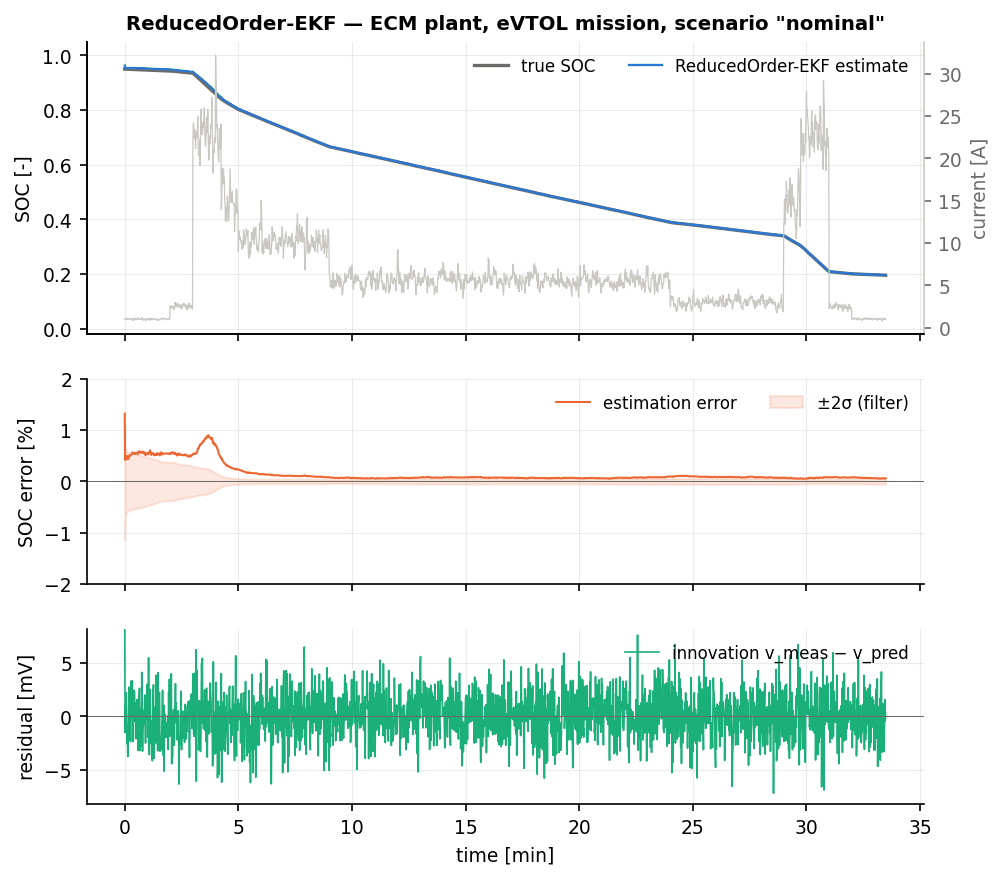
\includegraphics[width=\textwidth]{figures/cell_ReducedOrderEKF_nominal.png}
\caption{ReducedOrder-EKF on the nominal eVTOL mission: true and estimated SOC (top), estimation
error with the $\pm2\sigma$ band (middle), voltage residual (bottom).}
\end{figure}
\begin{figure}[H]\centering
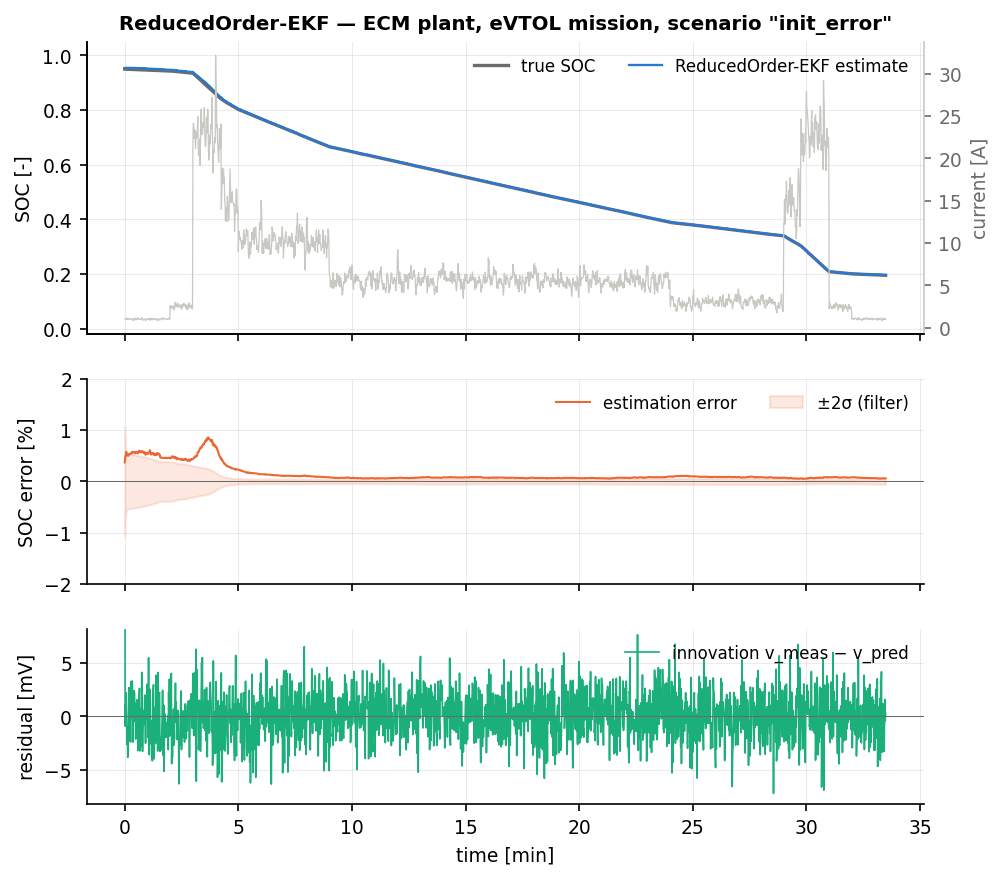
\includegraphics[width=\textwidth]{figures/cell_ReducedOrderEKF_init_error.png}
\caption{ReducedOrder-EKF with a 35\,\% initial SOC error.}
\end{figure}
\begin{figure}[H]\centering
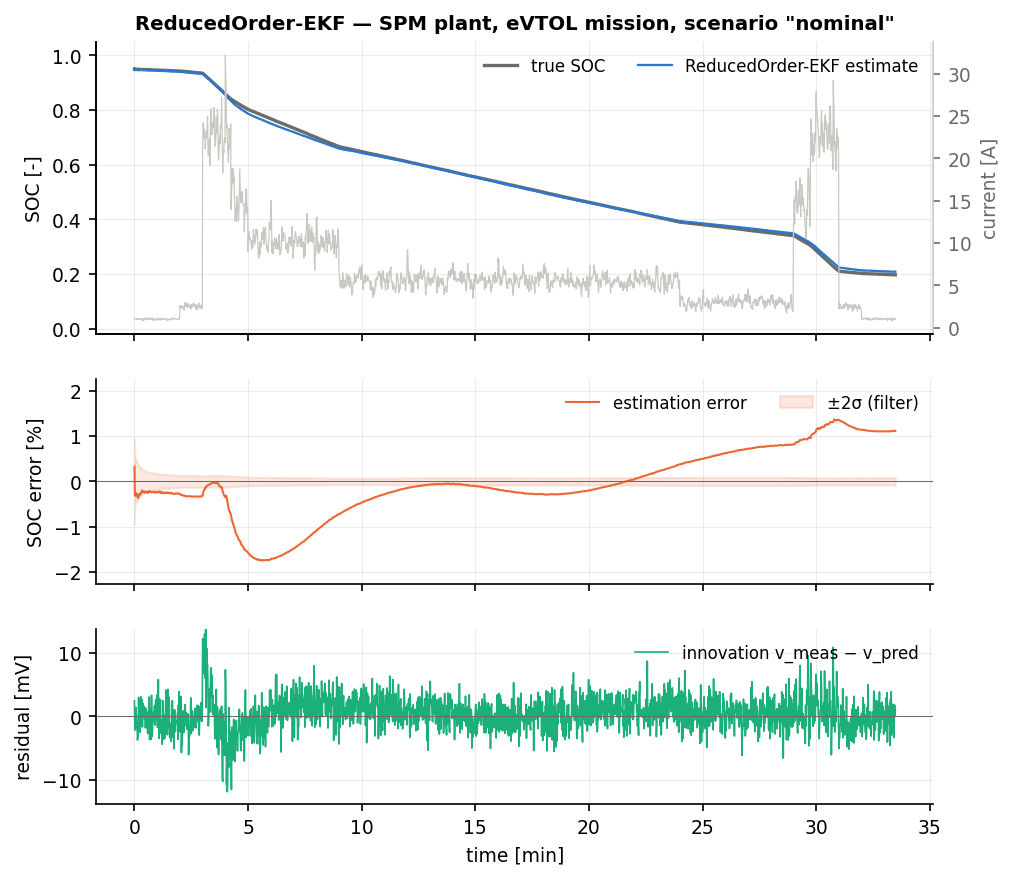
\includegraphics[width=\textwidth]{figures/cellspm_ReducedOrderEKF_nominal.png}
\caption{ReducedOrderEKF on the SPM (electrochemical) plant, nominal eVTOL mission.  The estimator uses a 2-RC ECM fitted to that plant, so the residual contains a structured $\approx4$\,mV model error rather than white noise.}
\end{figure}

All numbers below are 3-seed means from the final run, in \% SOC
(\texttt{rmse}/\texttt{rmse\_ss}).

\paragraph{ECM plant, eVTOL mission.}
\begin{center}\small
\begin{tabular}{@{}lccl@{}}
\toprule
Scenario & ReducedOrder-EKF & EKF ($n_x=4$) & Comment\\
\midrule
\texttt{nominal}        & $0.23/0.07$ & $0.15/0.05$ & $1.4\times$ worse --- the reduction cost\\
\texttt{init\_error}    & $0.22/0.07$ & $0.14/0.05$ & $t_\mathrm{conv}=0$\,s\\
\texttt{current\_bias}  & $1.08/0.85$ & $0.54/0.61$ & $1.4\times$ worse\\
\texttt{noise\_step}    & $0.23/0.10$ & $0.18/0.12$ & steady state slightly better\\
\texttt{outliers}       & $0.89/\mathbf{0.08}$ & $0.52/0.21$ & ss $2.6\times$ better, max $4.8\,\%$\\
\texttt{cold}           & $0.41/0.33$ & $0.20/0.16$ & $2\times$ worse\\
\texttt{hot}            & $0.17/\mathbf{0.02}$ & $0.20/0.03$ & ---\\
\texttt{aged\_cell}     & $3.22/2.12$ & $1.18/1.52$ & $1.4\times$ worse\\
\texttt{param\_mismatch}& $2.24/1.53$ & $1.28/1.36$ & $1.1\times$ worse\\
\texttt{sensor\_dropout}& $\mathbf{0.53/0.07}$ & $0.72/0.46$ & $\mathbf{6.6\times}$ better (ss)\\
\texttt{preisach}       & $1.04/0.99$ & $0.58/0.20$ & $5\times$ worse --- see below\\
\texttt{combined}       & $\mathbf{4.03/1.69}$ & $16.02/12.44$ & $\mathbf{7.4\times}$ better (ss); converges at 576\,s\\
\midrule
\multicolumn{2}{@{}l}{\textbf{ns/step}} & & $\mathbf{331}$ vs.\ $478$ ($-31\,\%$)\\
\multicolumn{2}{@{}l}{\textbf{$n_x$-dependent RAM}} & & $\mathbf{136}$\,B vs.\ $208$\,B ($-35\,\%$)\\
\bottomrule
\end{tabular}
\end{center}
Acceptance is met: \texttt{nominal} $\texttt{rmse\_ss}=0.07\,\%<2\,\%$, \texttt{init\_error}
$t_\mathrm{conv}=0$\,s, no divergence anywhere, worst ECM steady-state error $2.12\,\%$
(\texttt{aged\_cell}).

\paragraph{The accuracy cost.}  On clean data the reduced filter is $1.4\times$ less accurate in
steady state ($0.07\,\%$ vs.\ $0.05\,\%$).  Two mechanisms contribute and they can be separated:
with $\sigma_{v2}=0$ the single-seed nominal steady-state error is the same $0.08\,\%$, so the
inflated $\mR$ of \eqref{eq:ro-R} is \emph{not} the dominant term.  The rest comes from the loss of
the $v_2$ correction: the full EKF does use the measurement to adjust $v_2$ and, although that
adjustment is mostly noise, part of it correctly absorbs process-noise energy that the reduced
filter must now absorb through $\soc$.  The cost is largest where the slow branch matters most ---
\texttt{cold} ($2\times$: at $-10$\,\ensuremath{{}^\circ}C the Arrhenius factors make $R_2$ five
times and $\tau_2$ nearly four times their $25$\,\ensuremath{{}^\circ}C values, so the slow branch
reaches $\approx0.14$\,V during the take-off hover and its reconstruction error is the largest term
in the residual), \texttt{aged\_cell} ($1.4\times$) and \texttt{current\_bias} ($1.4\times$, where
a steady current offset produces a steady $v_2$ offset that the full filter can partly absorb).

\paragraph{Preisach.}  With the corrected plant sign convention \texttt{preisach} has become the
reduced model's worst relative result: $0.99\,\%$ against the EKF's $0.20\,\%$, and 77\,s to
converge against 16\,s.  The Preisach residual is a slowly varying voltage offset with no
current-proportional signature, i.e.\ exactly the shape that the full model's $v_2$ state can
absorb and the reduced model's fixed low-pass cannot.  This is the clearest single demonstration in
the chapter of what the dropped degree of freedom was actually doing: it was a low-frequency
residual sink, useful when the residual really is low-frequency and harmless noise otherwise.

\paragraph{The unexpected benefit.}  On \texttt{combined} the reduced filter is $7.4\times$ better
in steady state than the full EKF, on \texttt{sensor\_dropout} $6.6\times$ and on the steady-state
part of \texttt{outliers} $2.6\times$.  This is not the reduction being ``more accurate''; it is a
robustness effect and it is the same mechanism as the preceding paragraph read with the opposite
sign.  The full EKF's $v_2$ state is a free parameter with a very long time constant and almost no
observability, so when a large voltage residual appears --- the 200\,mV resistance error of the
aged cold cell, a 15\,s frozen sensor, a $\pm50$\,mV spike --- the filter has two ways to explain it
and the linearised update distributes the correction between $\soc$ and $v_2$ according to $\mP$,
not to physics.  Removing $v_2$ from the state removes that degree of freedom: the reduced filter
\emph{cannot} misattribute, so it degrades more gracefully.  Its \texttt{outliers} whole-run RMSE
($0.89\,\%$) and peak ($4.8\,\%$) are nevertheless worse than the EKF's, because a spike now has
nowhere to go but into $\soc$; the damage is transient, which is why the steady-state figure is the
better one.

\paragraph{SPM (electrochemical) plant.}  This is where the reduced model earns its place.  On the
SPM rows it gives $0.74/0.70\,\%$ on \texttt{nominal} against the EKF's $3.65/3.73\,\%$ --- a factor
of $5.3$ --- and it is essentially insensitive to the scenario: $0.70\,\%$ on \texttt{init\_error},
$0.71\,\%$ on \texttt{noise\_step}, $0.70\,\%$ on \texttt{outliers}, $0.70\,\%$ on
\texttt{sensor\_dropout} (against the EKF's $5.31\,\%$, $7.6\times$), $0.85\,\%$ on
\texttt{current\_bias} (against $5.69\,\%$, $6.7\times$), $0.64\,\%$ on \texttt{hot}.  Only
\texttt{cold} ($3.71\,\%$ vs.\ $7.35\,\%$) and \texttt{param\_mismatch} ($1.31\,\%$ vs.\
$3.13\,\%$) are above $1\,\%$.  Together with the Schmidt-KF ($0.51\,\%$) it is one of only two
filters in the family that break the $\approx3.7\,\%$ barrier at which every other estimator sits.

The mechanism is precisely the one identified above, now acting on a real model error rather than a
fault.  The SPM plant's $\approx4$\,mV structured residual is dominated by the concentration
overpotential, a slow, current-driven signal with a $\tau\approx556$\,s time constant --- which is
to say, it looks exactly like a slow RC branch that the fitted ECM does not get right.  A full 2-RC
EKF has a state, $v_2$, whose signature is indistinguishable from that residual over any window in
which the measurement is informative, and also indistinguishable from a slow drift in $\ocv(\soc)$.
Given a persistent residual of that shape the filter must split it between $v_2$ and $\soc$, and
because $\mP_{\soc\soc}$ is the larger of the two most of it lands on the SOC: hence the uniform
$3.1$--$4.1\,\%$ bias of the EKF and of every filter that keeps the fourth state.  The reduced model
has no $v_2$ to confuse with $\soc$; the slow branch is pinned to its open-loop value, the ambiguity
is structurally absent, and the residual is simply absorbed by the (deliberately inflated) $\mR$
instead of by the state.  The Schmidt-KF reaches the same place by a different route --- it inflates
$\mS$ so the ambiguous direction is never excited --- which is why those two, and only those two,
are immune.

The general lesson for model-order reduction is therefore stronger than the usual
flops-versus-accuracy trade: on a plant whose unmodelled physics resembles the state you removed,
removing it is not merely cheap but \emph{more accurate}, because a weakly observable state is a
liability in exactly the situation where the model is wrong.


\section{Summary}
Removing the slow RC branch from the estimator state and reconstructing it open loop costs
$1.4\times$ in steady-state SOC accuracy on clean ECM data and buys a $31\,\%$ reduction in CPU
time and a $35\,\%$ reduction in per-cell RAM --- the single cheapest way in this library to fit an
EKF-class estimator into a small MCU budget for a large pack, and the only estimator here that is
faster than the plain EKF.  It also, far from unexpectedly once the mechanism is understood, makes
the filter dramatically more robust wherever the residual is a slow, current-driven signal that the
missing state could have absorbed: $7.4\times$ better than the EKF on \texttt{combined} and
$5.3\times$ better on the electrochemical plant, where it and the consider filter are the only two
methods in this family that escape the $\approx3.7\,\%$ model-error floor.  Use it when the number
of cells, not the accuracy per cell, is the binding constraint; when the plant is richer than the
2-RC model used to estimate it; and when the mission has no long rests.  Do not use it when the
slow branch is genuinely observable (a chemistry with $\tau_2\approx20$\,s, a mission with
20-minute rests), where the \texttt{preisach} result --- $5\times$ worse than the full model --- is
the warning, and never with sigma-point or particle filters: the quasi-static branch is advanced
inside $\vf$ and assumes exactly one evaluation per sampling period.

% Copyright 2026 Sreeram Anil
% SPDX-License-Identifier: CC-BY-4.0
% =============================================================================
%  Smooth Variable Structure Filter — robust_kalman family
% =============================================================================
\providecommand{\vf}{\bm{f}} \providecommand{\vh}{\bm{h}}
\providecommand{\vd}{\bm{d}} \providecommand{\mM}{\bm{M}}
\providecommand{\va}{\bm{a}} \providecommand{\vb}{\bm{b}}

\chapter{Smooth variable structure filter (SVSF)}
\label{ch:svsf}

\section*{At a glance}
\begin{tabular}{@{}l>{\raggedright\arraybackslash}p{0.76\textwidth}@{}}
Family & Robust / embedded Kalman \\
Header & \texttt{include/estkit/filters/svsf.hpp} \\
Registered name & \texttt{SVSF} \\
State dimension & $n_x = 4$ (cell model) --- generic in $n_x, n_u, n_y$, requires $n_y\le n_x$ \\
Cost per step & $\mathcal{O}(n_x^3)$; 582\,ns/step, 4376\,B, no heap \\
Primary references & \cite{habibi2007svsf,gadsden2010svsfcov,utkin1992,gadsden2011svsfkf} \\
\end{tabular}

\section{Motivation and aerospace/BMS relevance}
Every filter in the preceding chapters is built on a \emph{stochastic} argument: a covariance is
propagated, a gain is derived from it, and the guarantee (optimality, consistency, minimax
variance) holds only as far as the assumed statistics do.  The smooth variable structure filter
comes from the other tradition.  It is a sliding-mode observer: the correction is a discontinuous
function of the output error, designed so that the output error is driven into a bounded region ---
the \emph{existence subspace} --- and kept there, \emph{regardless} of the modelling error, as long
as that error is bounded and the boundary layer is wide enough to contain it
\cite[\S III]{habibi2007svsf}, \cite{utkin1992}.  The stability proof needs no noise statistics at
all, only a bound.

That is an attractive property for a battery.  The dominant uncertainty in a cell model is not
noise but structure: an ohmic resistance that grows $25\,\%$ over life and varies by a factor of
five with temperature, a one-state hysteresis approximation of a Preisach operator, a capacity that
the BMS has not re-identified for two hundred cycles.  A Kalman filter tuned for the sensor noise
will happily diverge in the face of these; a sliding-mode corrector with a boundary layer chosen to
cover the \emph{model} error will not.  The SVSF also has a well-documented secondary benefit: the
magnitude of the chattering inside the boundary layer is a direct indicator of modelling error,
which makes it a natural fault-detection signal \cite{gadsden2011svsfkf}.

The difficulty for a cell estimator is that the SVSF was formulated for $n_y=n_x$ (a full-state
measurement).  Here $n_y=1$ and $n_x=4$.  Section~\ref{sec:sv-reduced} explains the choice made:
the SVSF-KF combination of Gadsden \& Habibi \cite{gadsden2010svsfcov}, in which the sliding-mode
law governs the observable direction and the EKF gain governs its complement.

\section{Problem statement and assumptions}
\begin{align}
\vx_{k+1}&=\vf(\vx_k,\vu_k)+\vw_k, & \vy_k&=\vh(\vx_k,\vu_k)+\vv_k, \label{eq:sv-model}
\end{align}
with $\vw,\vv$ \emph{unknown but bounded}; no distribution is assumed.  Define the a-priori and
a-posteriori output errors
\begin{equation}
\bm{e}_{k+1|k}=\vy_{k+1}-\vh(\xminus_{k+1},\vu_{k+1}),
\qquad
\bm{e}_{k|k}=\vy_{k}-\vh(\xplus_{k},\vu_{k}).
\label{eq:sv-e}
\end{equation}

\begin{assumption}[Existence subspace]\label{as:sv-psi}
There exists $\bm\psi\in\real^{n_y}_{>0}$ such that the combined effect of the measurement noise
and of the modelling error on the output residual is bounded by $\bm\psi$ in each channel.
$\bm\psi$ is the \emph{boundary layer} (or existence-subspace) width; it is a design parameter and
the only quantity the SVSF needs to know about the uncertainty.
\end{assumption}

\section{Derivation}

\subsection{The SVSF gain}
The SVSF correction in measurement space is \cite[Eq.~(29)]{habibi2007svsf}
\begin{equation}
\boxed{\;
\bm{k}^{\mathrm{svsf}}_{k+1}
 = \Big(\,\big|\bm{e}_{k+1|k}\big|_{\mathrm{abs}}
        + \gamma\,\big|\bm{e}_{k|k}\big|_{\mathrm{abs}}\Big)
   \circ \sat\!\Big(\frac{\bm{e}_{k+1|k}}{\bm\psi}\Big),\;}
\label{eq:sv-gain}
\end{equation}
where $|\cdot|_{\mathrm{abs}}$ is the element-wise absolute value, $\circ$ the Hadamard product,
$\sat(\cdot)$ the element-wise saturation
($\sat(s)=s$ for $|s|\le1$, $\sgn(s)$ otherwise) and $\gamma\in[0,1)$ the \emph{SVSF convergence
rate}.  The state correction $\delta\vx$ is applied so that
$\mH\,\delta\vx=\bm{k}^{\mathrm{svsf}}$ exactly.

\begin{theorem}[Sliding-mode convergence, Habibi 2007]\label{thm:sv-conv}
Assume $\mH\,\delta\vx=\bm{k}^{\mathrm{svsf}}$ and linearise $\vh$ about $\xminus$.  Then for
every channel $j$ with $|e_{j,k+1|k}|>\psi_j$,
\begin{equation}
e_{j,k+1|k+1}=e_{j,k+1|k}-k^{\mathrm{svsf}}_{j}
 = -\gamma\,|e_{j,k|k}|\,\sgn\!\big(e_{j,k+1|k}\big),
\qquad\text{so}\qquad
\big|e_{j,k+1|k+1}\big| = \gamma\,\big|e_{j,k|k}\big| .
\label{eq:sv-contract}
\end{equation}
The a-posteriori output error therefore contracts by the factor $\gamma<1$ at every step,
independently of $\vf$, $\vh$, $\mQ$, $\mR$ or the size of the modelling error, until it enters
the boundary layer $|e_j|\le\psi_j$.
\end{theorem}
\begin{proof}
Outside the layer $\sat(e/\psi)=\sgn(e)$, so
$k^{\mathrm{svsf}}_j=(|e_{k+1|k}|+\gamma|e_{k|k}|)\sgn(e_{k+1|k})$; substituting into
$e_{k+1|k+1}=e_{k+1|k}-k^{\mathrm{svsf}}_j$ and using
$e_{k+1|k}=|e_{k+1|k}|\sgn(e_{k+1|k})$ gives \eqref{eq:sv-contract}.
\end{proof}

This is the reachability/attractivity result of sliding-mode theory
($V_k=e_k^2$, $\Delta V_k<0$ outside the layer) written in discrete time.  Inside the layer
$\sat(e/\psi)=e/\psi$ and \eqref{eq:sv-gain} becomes
$k^{\mathrm{svsf}}_j=(|e_j|+\gamma|e_{j,k|k}|)\,e_j/\psi_j$, a \emph{quadratic} (hence very small)
correction --- this is the smoothing that removes the chattering of the plain VSF, at the price of
a low gain for small residuals.  The design trade is therefore entirely in $\bm\psi$: too small and
the filter tracks the measurement noise; too large and it becomes sluggish.

\subsection{More states than measurements}\label{sec:sv-reduced}
\eqref{eq:sv-gain} determines the correction only inside the $n_y$-dimensional row space of
$\mH$.  Habibi's original treatment assumes $n_y=n_x$; for $n_y<n_x$ he proposes a reduced-order
form, and Gadsden \& Habibi \cite{gadsden2010svsfcov} propose the \emph{SVSF-KF combination} used
here.  Let $\mH^{+}$ be any right inverse of $\mH$ ($\mH\mH^{+}=\mI_{n_y}$).  Then
\begin{equation}
\delta\vx \;=\; \underbrace{\mH^{+}\bm{k}^{\mathrm{svsf}}}_{\text{row space of }\mH:\ \text{SVSF}}
 \;+\; \underbrace{\big(\mI-\mH^{+}\mH\big)\,\mK^{\mathrm{EKF}}\bm{e}_{k+1|k}}_{%
   \text{null space of }\mH:\ \text{EKF}},
\label{eq:sv-split}
\end{equation}
which satisfies $\mH\,\delta\vx=\bm{k}^{\mathrm{svsf}}$ --- so Theorem~\ref{thm:sv-conv} still
holds --- while giving the $n_x-n_y=3$ unobserved directions the statistically motivated EKF
correction.  Two right inverses are offered:
\begin{equation}
\mH^{+}_{\mathrm{MP}}=\mH^\T\big(\mH\mH^\T\big)^{-1}
\quad\text{(Moore--Penrose)},
\qquad
\mH^{+}_{\mP}=\mP\mH^\T\big(\mH\mP\mH^\T\big)^{-1}
\quad\text{($\mP$-weighted, default)}.
\label{eq:sv-pinv}
\end{equation}
The default is the $\mP$-weighted one, and the reason is physical rather than numerical.  For the
cell model $\mH=[0.7,\,-1,\,-1,\,0.005]$, so $\mH^{+}_{\mathrm{MP}}\propto[0.28,-0.40,-0.40,0.002]$:
the Moore--Penrose inverse sends \emph{more} of the correction into $v_1,v_2$ than into $\soc$,
purely because the RC branches have a larger entry in $\mH$.  The $\mP$-weighted inverse sends it
along $\mP\mH^\T$, i.e.\ in the Kalman direction, normalised so that the output residual moves by
exactly $\bm{k}^{\mathrm{svsf}}$ --- the same direction as the EKF but with the sliding-mode
\emph{magnitude}.  That is precisely the SVSF-KF idea.

\subsection{Covariance}
Because \eqref{eq:sv-gain} is homogeneous of degree one in $\bm{e}$ when written with the ratios
\begin{equation}
\rho_j = \frac{|e_j|+\gamma|e_{j,k|k}|}{\max(\psi_j,\,|e_j|)}
       = \begin{cases}
         \big(|e_j|+\gamma|e_{j,k|k}|\big)/\psi_j, & |e_j|\le\psi_j,\\[2pt]
         \big(|e_j|+\gamma|e_{j,k|k}|\big)/|e_j|, & |e_j|>\psi_j,
         \end{cases}
\label{eq:sv-ratio}
\end{equation}
one has $\bm{k}^{\mathrm{svsf}}=\diag(\bm\rho)\,\bm{e}$ with no division by zero ($\psi_j>0$ in the
first branch, $|e_j|>\psi_j>0$ in the second), and the whole update is a linear gain
\begin{equation}
\mK^{\mathrm{eff}}_{k}=\mH^{+}\diag(\bm\rho)+\big(\mI-\mH^{+}\mH\big)\mK^{\mathrm{EKF}},
\qquad \delta\vx=\mK^{\mathrm{eff}}_k\,\bm{e}_{k+1|k}.
\label{eq:sv-Keff}
\end{equation}
The covariance can then be propagated with the Joseph form of the gain that was \emph{actually}
applied,
\begin{equation}
\Pplus_k=\big(\mI-\mK^{\mathrm{eff}}\mH\big)\Pminus_k\big(\mI-\mK^{\mathrm{eff}}\mH\big)^\T
        +\mK^{\mathrm{eff}}\mR_k\big(\mK^{\mathrm{eff}}\big)^\T,
\label{eq:sv-P}
\end{equation}
which is the covariance derivation of \cite{gadsden2010svsfcov}.  $\Pplus$ is used for two things:
to build $\mH^{+}_{\mP}$ and $\mK^{\mathrm{EKF}}$ for the next step, and to report a SOC standard
deviation.  It is an honest error covariance of the applied linear gain under Gaussian noise ---
not an optimal one, because $\mK^{\mathrm{eff}}$ is not the Kalman gain.

\begin{remark}[Relation to the other robust filters]\label{rem:sv-rel}
Huber, MCKF and the Student's t filter all \emph{reduce} the gain when the residual is large.  The
SVSF does the opposite outside the boundary layer: $\rho_j\ge1$, so it drives the residual to zero
(and slightly beyond, by $\gamma|e_{k|k}|$) no matter how large it is.  It is therefore the natural
tool against \emph{model} error --- where the residual is real information that must be acted on
--- and the wrong tool against measurement outliers, where the residual is noise.  The benchmark
below shows exactly this split.
\end{remark}

\section{Algorithm}
\begin{algorithm}[H]
\caption{SVSF (SVSF-KF form) --- one sampling period}
\begin{algorithmic}[1]
\Require $\xplus_{k-1},\Pplus_{k-1},\bm{e}_{k-1|k-1},\vu_{k-1},\vy_k,\vu_k,\gamma,\bm\psi$
\State \textbf{Time update:} $\mF\gets\partial\vf/\partial\vx$;\;
  $\xminus_k\gets\vf(\xplus_{k-1},\vu_{k-1})$;\;
  $\Pminus_k\gets\mF\Pplus_{k-1}\mF^\T+\mQ_k$; symmetrise
\State \textbf{Measurement update:} $\mH\gets\partial\vh/\partial\vx$;\; $\mR\gets\mR_k$
\State $\bm{e}_{k|k-1}\gets\vy_k-\vh(\xminus_k,\vu_k)$ \Comment{a-priori residual}
\State $\mS\gets\mH\Pminus_k\mH^\T+\mR$;\quad
  $\mK^{\mathrm{EKF}}\gets\Pminus_k\mH^\T\mS^{-1}$
\State $\mH^{+}\gets\Pminus_k\mH^\T(\mH\Pminus_k\mH^\T)^{-1}$ \Comment{Eq.~\eqref{eq:sv-pinv}}
\For{$j=1,\dots,n_y$}
  \State $\psi_j\gets\max\big(\psi^{\mathrm{abs}}_j,\ \psi^{\sigma}\sqrt{\mR_{jj}}\big)$
  \State $\rho_j\gets$ \eqref{eq:sv-ratio} using $|e_{j}|$ and the stored $|e_{j,k-1|k-1}|$
\EndFor
\State $\mK^{\mathrm{eff}}\gets\mH^{+}\diag(\bm\rho)+(\mI-\mH^{+}\mH)\mK^{\mathrm{EKF}}$
       \Comment{Eq.~\eqref{eq:sv-Keff}}
\State $\xplus_k\gets\xminus_k+\mK^{\mathrm{eff}}\bm{e}_{k|k-1}$
\State $\Pplus_k\gets(\mI-\mK^{\mathrm{eff}}\mH)\Pminus_k(\mI-\mK^{\mathrm{eff}}\mH)^\T
       +\mK^{\mathrm{eff}}\mR(\mK^{\mathrm{eff}})^\T$; symmetrise; \code{constrain}
\State $\bm{e}_{k|k}\gets\vy_k-\vh(\xplus_k,\vu_k)$ \Comment{store for the next step}
\Ensure $\xplus_k,\Pplus_k,\bm{e}_{k|k}$
\end{algorithmic}
\end{algorithm}

\section{Application to the battery model}
Two parameters must be chosen.

\paragraph{Boundary layer $\psi$.}  Assumption~\ref{as:sv-psi} says $\psi$ must cover the
\emph{modelling} error, not only the sensor noise --- a point Habibi makes repeatedly and which is
the most common way to get the SVSF wrong.  For this cell:
\begin{center}\small
\begin{tabular}{@{}lr@{}}
\toprule
Contribution to the voltage residual & magnitude \\
\midrule
voltage sensor noise + 1\,mV ADC quantisation & $\approx2.1$\,mV\\
$20\,\%$ uncertainty in $R_0$ at the 22.5\,A hover current & $54$\,mV\\
$25\,\%$ resistance growth of an aged cell at 22.5\,A & $67$\,mV\\
one-state approximation of the Preisach hysteresis & $\approx10$\,mV\\
$50\,\%$ error in $\tau_2$ during a 75\,s hover & $23$\,mV\\
\midrule
\textbf{registered} $\psi$ & $\bm{100}$\,\textbf{mV}\\
\bottomrule
\end{tabular}
\end{center}
The generic default in \code{Options} is $\psi_j=\psi^\sigma\sqrt{\mR_{jj}}$ with
$\psi^\sigma=5$, which auto-scales to any model; the registration overrides it with the
battery-specific absolute value $\psi^{\mathrm{abs}}=100$\,mV
($\approx48\sqrt{\mR}$).  A sweep over $\psi\in\{2,5,10,20,30,40,50,60,65,80,100\}\sqrt{\mR}$ and
$\gamma\in\{0.05,\dots,0.9\}$ shows the trade cleanly (single seed, \% SOC): at
$\psi=5\sqrt{\mR}$ the filter is inside the sliding mode most of the time and \texttt{outliers}
diverges ($\texttt{rmse}=38\,\%$), at $\psi=20\sqrt{\mR}$ \texttt{param\_mismatch} is best but
\texttt{outliers} still diverges, and from $\psi\approx50\sqrt{\mR}$ upwards no ECM scenario
diverges and \texttt{combined} settles at $\texttt{rmse\_ss}\approx2\,\%$.  Around the registered
value the residual sensitivity is small but not negligible: over
$\psi^{\mathrm{abs}}\in\{90,100,110,120\}$\,mV the single-seed \texttt{outliers} steady-state error
moves between $0.65\,\%$ and $3.1\,\%$ while \texttt{combined} stays within
$1.6$--$2.3\,\%$ --- the \texttt{outliers} figure is the one that is chaotic, because a spike that
lands near the layer boundary switches branch.

\paragraph{Convergence rate $\gamma$.}  Habibi's range is $0\le\gamma<1$; the registered value is
$0.20$.  Larger $\gamma$ makes the sliding mode overshoot more (the residual is driven to
$-\gamma|e_{k|k}|$ rather than to zero), which on noisy data injects noise; smaller $\gamma$ makes
the filter slower to leave the boundary layer.  The measured sensitivity is modest: over
$\gamma\in\{0.1,0.2,0.3\}$ at $\psi=100$\,mV the single-seed \texttt{combined} steady-state error
varies between $1.64\,\%$ and $1.99\,\%$ and \texttt{nominal} stays at $0.04$--$0.05\,\%$.

\section{Implementation notes}
\begin{itemize}[nosep]
\item \textbf{Cost.}  One EKF gain, one $\mH^{+}$ (an $n_y\times n_y$ inverse plus an
$n_x\times n_y$ product), one $n_x\times n_x$ projector and one Joseph form.  Measured
582\,ns/step against 478\,ns for the EKF ($1.22\times$); memory 4376\,B against 4336\,B.
\item \textbf{No division by zero.}  Working with the ratios \eqref{eq:sv-ratio} rather than with
$\bm{k}^{\mathrm{svsf}}/\bm{e}$ removes the singularity at $\bm{e}=\bm0$ analytically, which
matters because the residual crosses zero constantly in normal operation.
$\mH\Pminus\mH^\T$ is regularised by $10^{-30}$ before inversion in case $\mP$ collapses.
\item \textbf{The stored a-posteriori residual.}  $\bm{e}_{k|k}$ is recomputed after the state
update with the \emph{nonlinear} $\vh$, so the contraction \eqref{eq:sv-contract} is measured on
the true output error and not on its linearisation.
\item \textbf{$\gamma$ and $\psi$ are the only tuning knobs} and both have physical meaning
(a contraction rate and an uncertainty bound).  There is no covariance to tune, which is the
practical appeal of the method.
\item \textbf{float32.}  Stable, but more sensitive than the other filters: \texttt{nominal}
$0.18/0.05\,\%$ (double $0.18/0.04\,\%$), \texttt{combined} $4.59/1.98\,\%$ (double
$4.65/1.91\,\%$), but \texttt{outliers} degrades from $2.31/1.80\,\%$ to $5.97/4.41\,\%$; the
footprint halves to 2188\,B.  The
sensitivity comes from the $\sat$ switching: a residual that sits exactly at the boundary switches
branch differently in the two precisions, and the SVSF has no covariance damping to smooth the
difference.
\item \textbf{Cortex-M7 estimate.}  $\approx900$ flops/step; $\approx5\,\mu$s at 300\,MHz.
\item \textbf{Limitation.}  As Remark~\ref{rem:sv-rel} explains, the SVSF amplifies rather than
rejects large measurement residuals.  It must not be used on a channel that can produce gross
errors unless it is preceded by a gate or combined with an $M$-estimator.
\end{itemize}

\section{Benchmark results}
% Copyright 2026 Sreeram Anil
% SPDX-License-Identifier: CC-BY-4.0
\begin{table}[H]\centering\footnotesize\setlength{\tabcolsep}{4pt}
\caption{SVSF: cell-level benchmark on the eVTOL mission (mean over seeds; RMSE and max error in \% SOC; $t_\mathrm{conv}$: first time the error stays below 2\,\% for 60\,s, -- = never; EKF reference: steady-state RMSE of the plain EKF on the same data).}\label{tab:cell_SVSF}
\begin{tabular}{llrrrrrcrr}\toprule
plant & scenario & RMSE & RMSE$_\mathrm{ss}$ & max & $t_\mathrm{conv}$ [s] & RMSE$_v$ [mV] & div. & EKF ref. & ns/step \\ \midrule
ECM & nominal & 0.18 & 0.04 & 0.68 & 0 & 0.78 & no & 0.05 & 583 \\
ECM & init\_error & 0.17 & 0.04 & 0.70 & 0 & 2.12 & no & 0.05 & 585 \\
ECM & current\_bias & 0.58 & 0.55 & 1.51 & 0 & 0.90 & no & 0.61 & 584 \\
ECM & noise\_step & 1.39 & 1.71 & 4.55 & 0 & 8.84 & no & 0.12 & 585 \\
ECM & outliers & 2.31 & 1.80 & 6.51 & 9 & 9.08 & no & 0.21 & 587 \\
ECM & cold & 0.31 & 0.11 & 1.06 & 0 & 1.90 & no & 0.16 & 584 \\
ECM & hot & 0.18 & 0.03 & 0.67 & 0 & 0.52 & no & 0.03 & 586 \\
ECM & aged\_cell & 1.21 & 1.02 & 4.77 & 0 & 2.76 & no & 1.52 & 588 \\
ECM & param\_mismatch & 1.82 & 1.75 & 4.18 & 0 & 2.21 & no & 1.36 & 583 \\
ECM & sensor\_dropout & 0.99 & 0.58 & 3.37 & 0 & 2.00 & no & 0.46 & 583 \\
ECM & preisach & 0.77 & 0.22 & 2.59 & 212 & 0.83 & no & 0.20 & 582 \\
ECM & combined & 4.65 & 1.91 & 13.06 & 1398 & 3.37 & no & 12.44 & 586 \\
\midrule
SPM & nominal & 3.68 & 3.73 & 4.54 & 0 & 1.04 & no & 3.73 & 552 \\
SPM & init\_error & 3.94 & 3.93 & 4.97 & 0 & 2.19 & no & 3.81 & 550 \\
SPM & current\_bias & 5.15 & 5.87 & 6.61 & 0 & 1.15 & no & 5.69 & 556 \\
SPM & noise\_step & 12.40 & 17.24 & 24.67 & 0 & 8.91 & no & 3.30 & 555 \\
SPM & outliers & 14.10 & 17.12 & 19.22 & 76 & 9.18 & yes & 1.99 & 543 \\
SPM & cold & 6.82 & 6.91 & 9.18 & -- & 3.10 & no & 7.35 & 554 \\
SPM & hot & 2.37 & 2.37 & 2.96 & 0 & 0.72 & no & 2.16 & 552 \\
SPM & param\_mismatch & 3.89 & 4.08 & 4.79 & 0 & 1.71 & no & 3.13 & 554 \\
SPM & sensor\_dropout & 5.88 & 6.06 & 6.78 & 0 & 2.07 & no & 5.31 & 552 \\
\bottomrule\end{tabular}\end{table}

\begin{figure}[H]\centering
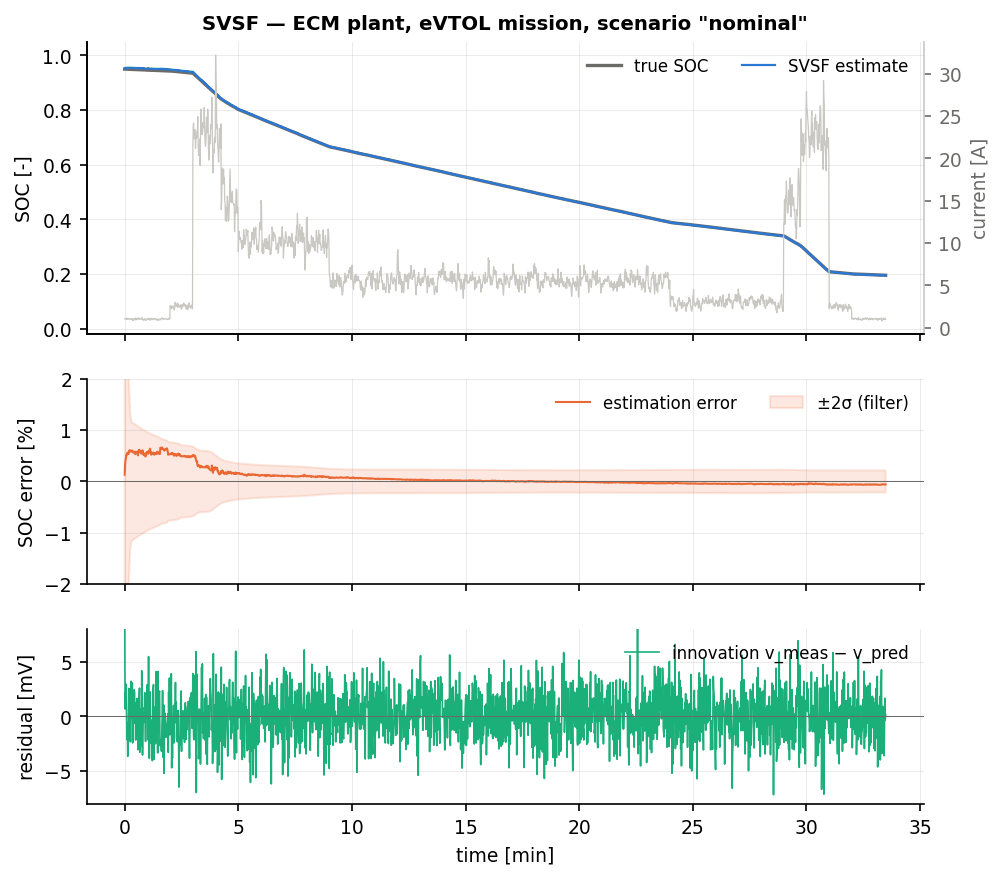
\includegraphics[width=\textwidth]{figures/cell_SVSF_nominal.png}
\caption{SVSF on the nominal eVTOL mission: true and estimated SOC (top), estimation error with the
$\pm2\sigma$ band from the SVSF-KF covariance (middle), voltage residual (bottom).}
\end{figure}
\begin{figure}[H]\centering
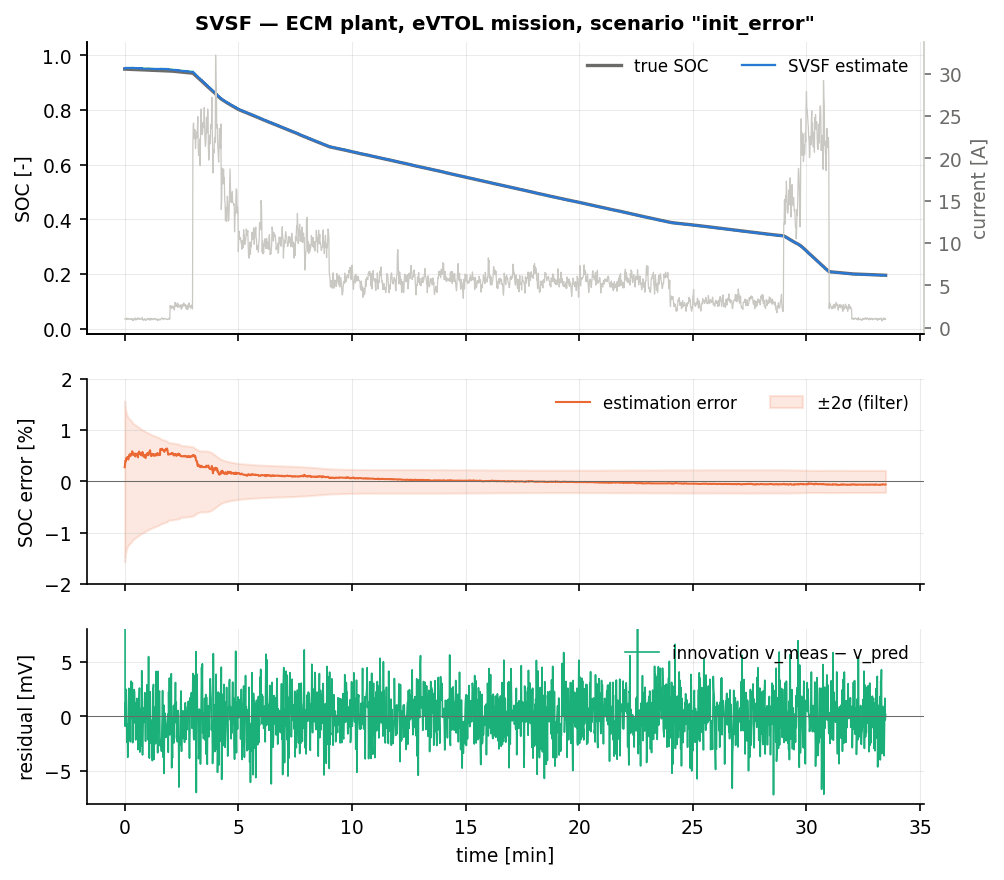
\includegraphics[width=\textwidth]{figures/cell_SVSF_init_error.png}
\caption{SVSF with a 35\,\% initial SOC error.}
\end{figure}
\begin{figure}[H]\centering
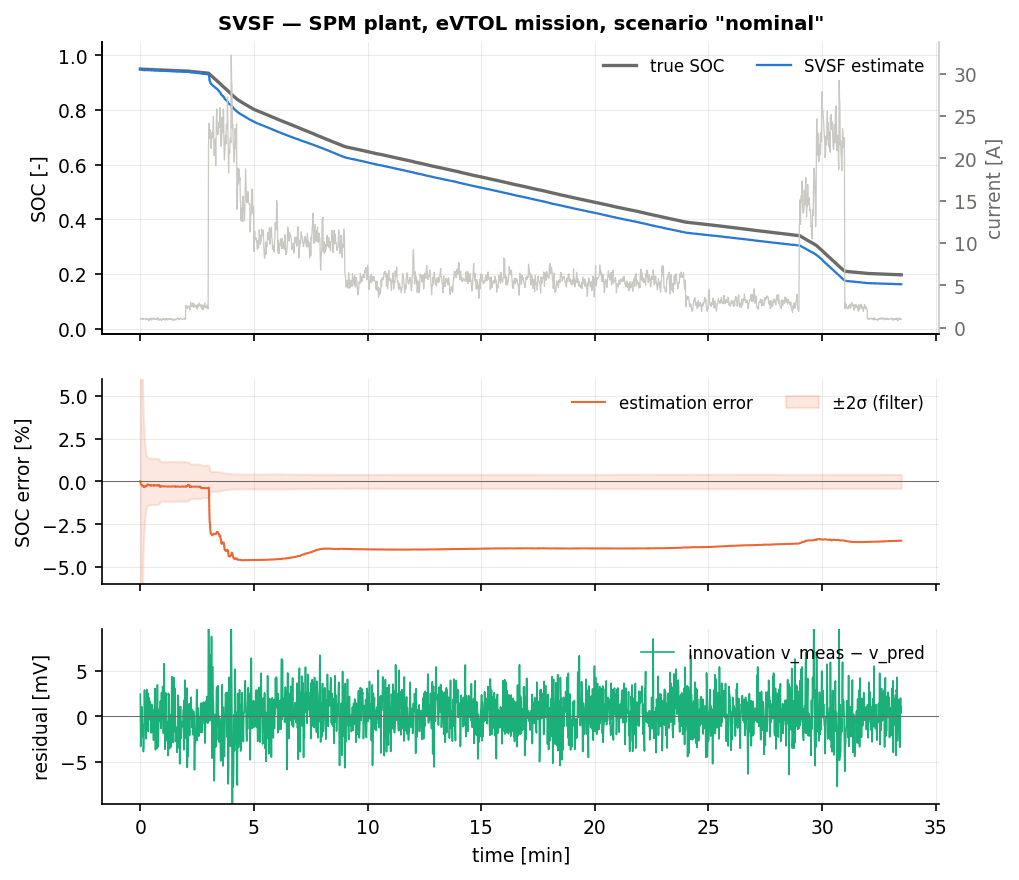
\includegraphics[width=\textwidth]{figures/cellspm_SVSF_nominal.png}
\caption{SVSF on the SPM (electrochemical) plant, nominal eVTOL mission.  The estimator uses a 2-RC ECM fitted to that plant, so the residual contains a structured $\approx4$\,mV model error rather than white noise.}
\end{figure}

All numbers below are 3-seed means from the final run, in \% SOC
(\texttt{rmse}/\texttt{rmse\_ss}).

\paragraph{ECM plant, eVTOL mission.}
\begin{center}\small
\begin{tabular}{@{}lccl@{}}
\toprule
Scenario & SVSF & EKF & Comment\\
\midrule
\texttt{nominal}        & $0.18/\mathbf{0.04}$ & $0.15/0.05$ & same ss; max error $0.68\,\%$ vs.\ $1.07\,\%$\\
\texttt{init\_error}    & $0.17/\mathbf{0.04}$ & $0.14/0.05$ & $t_\mathrm{conv}=0$\,s\\
\texttt{current\_bias}  & $0.58/\mathbf{0.55}$ & $0.54/0.61$ & marginally better (ss)\\
\texttt{noise\_step}    & $1.39/1.71$ & $0.18/0.12$ & $14\times$ worse --- see below\\
\texttt{outliers}       & $2.31/1.80$ & $0.52/0.21$ & $8.6\times$ worse --- see below\\
\texttt{cold}           & $0.31/\mathbf{0.11}$ & $0.20/0.16$ & $1.5\times$ better (ss)\\
\texttt{hot}            & $0.18/0.03$ & $0.20/0.03$ & ---\\
\texttt{aged\_cell}     & $1.21/\mathbf{1.02}$ & $1.18/1.52$ & $1.5\times$ better (ss)\\
\texttt{param\_mismatch}& $1.82/1.75$ & $1.28/1.36$ & $1.29\times$ \emph{worse}\\
\texttt{sensor\_dropout}& $0.99/0.58$ & $0.72/0.46$ & $1.3\times$ worse\\
\texttt{preisach}       & $0.77/0.22$ & $0.58/0.20$ & tied; $t_\mathrm{conv}$ 212\,s vs.\ 16\,s\\
\texttt{combined}       & $\mathbf{4.65/1.91}$ & $16.02/12.44$ & $\mathbf{6.5\times}$ better (ss); converges at 1398\,s\\
\bottomrule
\end{tabular}
\end{center}
Acceptance is met on the ECM plant: \texttt{nominal} $\texttt{rmse\_ss}=0.04\,\%<2\,\%$,
\texttt{init\_error} $t_\mathrm{conv}=0$\,s, no ECM divergence.  The worst ECM steady-state error is
$1.91\,\%$ (\texttt{combined}).  On the SPM plant the filter \textbf{diverges on \texttt{outliers}}
(flagged in the table); see below.

\paragraph{Target scenarios.}  \texttt{combined} is the headline: $1.91\,\%$ steady state against
the EKF's $12.44\,\%$, a factor of $6.5$, and the filter converges at $t=1398$\,s where the EKF
never does.  This is Theorem~\ref{thm:sv-conv} doing exactly what it promises: the 200\,mV
voltage-prediction error produced by the aged, cold cell during the take-off hover is far outside
the 100\,mV boundary layer, the sliding-mode corrector drives it back regardless of the fact that
the model is wrong, and the filter recovers.  \texttt{aged\_cell} improves $1.5\times$ in steady
state and \texttt{cold} $1.5\times$ for the same reason; the \texttt{nominal} peak error is the
lowest in the family ($0.68\,\%$ against the EKF's $1.07\,\%$), because the correction magnitude is
bounded by construction rather than by a covariance.

\texttt{param\_mismatch}, the other nominated scenario, is now $1.29\times$ \emph{worse} than the
EKF ($1.75\,\%$ vs.\ $1.36\,\%$; in the development run it was a tie).  The cause is visible in the
numbers: there the residual is a current-proportional bias that during cruise
($5.5$\,A $\times$ $3.6$\,m\ensuremath{\Omega} $=20$\,mV) sits well \emph{inside} the boundary
layer, so the filter runs in its smooth, quadratic, low-gain regime and simply tracks more slowly
than the EKF without gaining any sliding-mode protection.  Shrinking $\psi$ to $20\sqrt{\mR}=42$\,mV
does not help --- \texttt{param\_mismatch} barely moves while \texttt{outliers} diverges --- so
there is nothing to gain there, and the honest statement is that the SVSF wins on
\texttt{combined} and \texttt{aged\_cell} but not on \texttt{param\_mismatch}.

\paragraph{The two failures, and why they are the same failure.}  \texttt{outliers}
($8.6\times$ worse) and \texttt{noise\_step} ($14\times$ worse) are the mirror image of the wins.
Remark~\ref{rem:sv-rel} explains it: outside the boundary layer $\rho_j\ge1$, so the SVSF drives
the residual to zero \emph{whatever caused it}, and inside the layer the quadratic gain
$\rho\approx(|e|+\gamma|e_{k|k}|)/\psi$ is still non-zero.  A $\pm50$\,mV spike is a residual of
$24\sigma$ but only $0.5\psi$, so it is attenuated rather than amplified --- which is why the
failure is a factor of nine and not a divergence --- but the 20\,mV sensor noise of
\texttt{noise\_step} is a sustained excitation of the in-layer gain and the SOC then tracks the
noise.  The remedy is not a different $\psi$ (the sweep shows the trade is monotone) but a different
filter: on \texttt{outliers} the MC-EKF of Chapter~\ref{ch:mcekf} gives $0.12\,\%$, and a practical
design would place an $M$-estimator gate in front of the SVSF.

\paragraph{Structural choices.}  Replacing the $\mP$-weighted right inverse by the Moore--Penrose
one improves \texttt{nominal}, \texttt{current\_bias} and \texttt{aged\_cell} but costs a factor of
two on \texttt{noise\_step} and \texttt{combined}; the $\mP$-weighted inverse is kept because it is
the only one whose correction direction has a statistical justification and because it gives the
better worst case.  Disabling the null-space EKF term in \eqref{eq:sv-split} changes nothing
measurable on this model, which is consistent with $\mK^{\mathrm{EKF}}$ being almost parallel to
$\mP\mH^\T$ --- i.e.\ for $n_y=1$ and a $\mP$-weighted inverse the two terms nearly coincide.

\paragraph{SPM (electrochemical) plant, including a divergence.}  The SPM rows are the SVSF's worst
result in the benchmark and the only divergence anywhere in this family.  On \texttt{nominal} it
gives $3.68/3.73\,\%$ --- indistinguishable from the EKF's $3.65/3.73\,\%$ --- and on
\texttt{param\_mismatch} $4.08\,\%$ against $3.13\,\%$, \texttt{sensor\_dropout} $6.06\,\%$ against
$5.31\,\%$, \texttt{current\_bias} $5.87\,\%$ against $5.69\,\%$: worse than the EKF on six of nine
scenarios.  On \texttt{noise\_step} it reaches $12.40/17.24\,\%$ and on \texttt{outliers}
$14.10/17.12\,\%$ with \texttt{diverged}$=1$.

Two things combine to produce this.  First, the $\approx4$\,mV structured residual of the SPM plant
is far \emph{inside} the 100\,mV boundary layer, so the sliding-mode term never activates and the
SVSF degenerates to a low-gain filter with no protection at all --- exactly the
\texttt{param\_mismatch} mechanism above, now applying to every SPM scenario.  The boundary layer
was sized for the ECM's 20\,\% $R_0$ uncertainty at hover currents; it is an order of magnitude too
wide for a 4\,mV model error, and no single $\psi$ can be right for both.  Second, on
\texttt{noise\_step} and \texttt{outliers} the in-layer quadratic gain is excited by a 20\,mV noise
floor or by $\pm50$\,mV spikes on top of a filter that is already biased by $\approx3.7\,\%$; with
no covariance to damp it, the SOC estimate walks, and the metric's $30\,\%$ divergence threshold is
crossed.  This is the sharpest illustration available of the SVSF's defining trade: a corrector
whose magnitude is set by a \emph{bound} rather than by a \emph{statistic} is unbeatable when the
bound is right and has no fallback when it is not.  A production design would schedule $\psi$ with
the current (making it $\psi_0+|i|\,\sigma_{R_0}$ rather than a constant), which would restore the
ECM behaviour and give the SPM rows a layer of the right order; that variant is not implemented
here.


\section{Summary}
The SVSF is the only filter in this family whose convergence proof does not mention a covariance:
outside the boundary layer the output residual contracts by $\gamma$ per step regardless of how
wrong the model is.  That makes it one of the strongest performers here on \texttt{combined}
($6.5\times$ better than the EKF) and on \texttt{aged\_cell}, and a reasonable choice whenever
structured model error \emph{large enough to leave the boundary layer} is the dominant uncertainty
--- an aged pack, a badly calibrated resistance, a cold start.  Set $\psi$ from the \emph{model}
error budget (100\,mV here, fifty times the sensor noise), not from the sensor specification, and
schedule it with the current if the operating envelope is wide.  Do not use it where the
measurement can be grossly wrong: the same mechanism that rejects model error faithfully reproduces
an outlier, and \texttt{outliers} and \texttt{noise\_step} are the two ECM scenarios where it is
dramatically worse than a plain EKF.  And do not use a fixed $\psi$ across plants: on the
electrochemical plant, whose 4\,mV residual is two orders of magnitude inside the layer sized for
the ECM, the filter is no better than the EKF on seven scenarios and is the only estimator in this
family to diverge (SPM \texttt{outliers}).

